\documentclass[11pt,twoside,openright,fleqn,a4paper]{book}
\usepackage{eimthesis, symbols, graphicx, color, bibentry,nomencl}
\usepackage{amsfonts}
\usepackage{listings}
\usepackage[chapter,boxed]{algorithm}
\usepackage[noend]{algorithmic}
\usepackage[numbers,sort&compress]{natbib}
\usepackage{captionfont}
%\usepackage[bookmarks=true]{hyperref}
\pagestyle{plain}
\makenomenclature
\newcommand{\theHalgorithm}{\theHchapter.\arabic{algorithm}}

\begin{document}
\pagenumbering{roman}

\title{Animation of Captured Surface Data}
\author{Raymond James Smith}
\centre{Centre for Vision, Speech and Signal Processing}

\renewcommand{\month}{9}
\renewcommand{\year}{2003}

\summary{
\renewcommand{\baselinestretch}{1.5}\normalsize
Creation of 3D graphical content becomes ever harder, as both display capabilities and the demand for complex 3D content increase. In this thesis, we present a method of using densely scanned surface data from physical objects in interactive animation systems. By using a layered approach, incorporating skeletal animation and displacement mapping, we can realistically animate complex datasets with a minimum of manual intervention. 

We propose a method using three layers; firstly, an articulated skeleton layer provides simple motion control of the object. Secondly, a low-polygon control layer, based on the scanned surface, is mapped to this skeleton, and animated using a novel geometric skeletal animation method. Finally, the densely sampled surface mesh is mapped to this control layer using a normal volume mapping, forming the detail layer of the system. This mapping allows animation of the dense mesh data based on deformation of the control layer beneath. The complete layered animation chain allows an animator to perform interactive animation using the control layer, the results of which can then be used to automatically animate a highly detailed surface for final rendering. 

We also propose an extension to this method, in which the detail layer is replaced by a displacement map defined over the control layer. This enables dynamic level of detail rendering, allowing realtime rendering of the dense data, or an approximation thereof. This representation also supports such applications as simple surface editing and compression of surface data. We describe a novel displacement map creation technique based on normal volume mapping, and analyse the performance and accuracy of this method.

\renewcommand{\baselinestretch}{1}\normalsize
}
\keywords{layered animation, skeletal animation, normal volume mapping, displacement mapping}
\email{r.j.smith@acm.org}

\acknowledgements{
\renewcommand{\baselinestretch}{1.5}\normalsize
Many thanks to all of those who have supported me through this research. In particular, I'd like to thank my supervisor, Adrian Hilton, for accepting me in the first place, for putting up with my various flights of fancy along the way, and without whom I would perhaps never have discovered the fascinating field of computer graphics. Thanks also to Wei Sun, for collaboration during the early years, and to Gordon Collins for carrying on brilliantly where Wei left off.

I should also thank the various companies who have offered advice and direction along the way. Thanks go to 3D Scanners and Avatar-Me, for listening to my mad ideas on seamless animation, Bulgarian programming support, and one particularly large wooden paperweight. Thanks as well to both Jim Henson's Creature Shop and FrameStore, for letting us see how their model creation processes worked, and suggesting ways we could improve their lot.

There are also many people who have supported me in non-academic ways over this time. Everyone at OmniPerception deserves many thanks for making these last couple of months a lot easier, and making this thesis a much better piece of work than it might have been otherwise. To Warren Moore, I owe thanks for many great ideas (and a few not so great), and I probably owe a whole lot of beers to the Wates House drinking crew, for always keeping me somewhere near reality. You know who you are.

Finally, and most importantly, I'd like to say a huge thankyou to my partner Amanda, for putting up with this (and me) for far too many years, and for proofreading a 150-page document that made no sense. Sorry it took so long!

This project was supported by EPSRC Grant GR/89518 `Functional Models: Building Realistic Models for Virtual Reality and Animation'.

James Smith

September 2003
\renewcommand{\baselinestretch}{1}\normalsize
}

\makefront
\tableofcontents
\listoffigures
\listoftables
\renewcommand{\baselinestretch}{1.5}\normalsize
\listofsymbols
\renewcommand{\nomname}{Glossary}
\printnomenclature

\cleardoublepage
\pagestyle{headings}
\pagenumbering{arabic}
\nobibliography*

\chapter{\label{sec:introduction}Introduction}

Over recent years, the continuing increase in available computing power, coupled with the public's ever-increasing thirst for entertainment, has made the use of three-dimensional computer graphics commonplace. From film and television production, through to games and Internet-based shopping, the demand for highly realistic 3D content is increasing at an enormous rate. The computing power available to display such 3D content doubles roughly every 18 months, in line with Moore's Law, a trend which shows no sign of abating. Today's personal computers are capable of creating images more realistic than was possible with the most advanced supercomputers 10 years ago (see figure \ref{fig:3dgraphics} for some examples).

\begin{figure}
\begin{center}
\begin{tabular}{ccc}
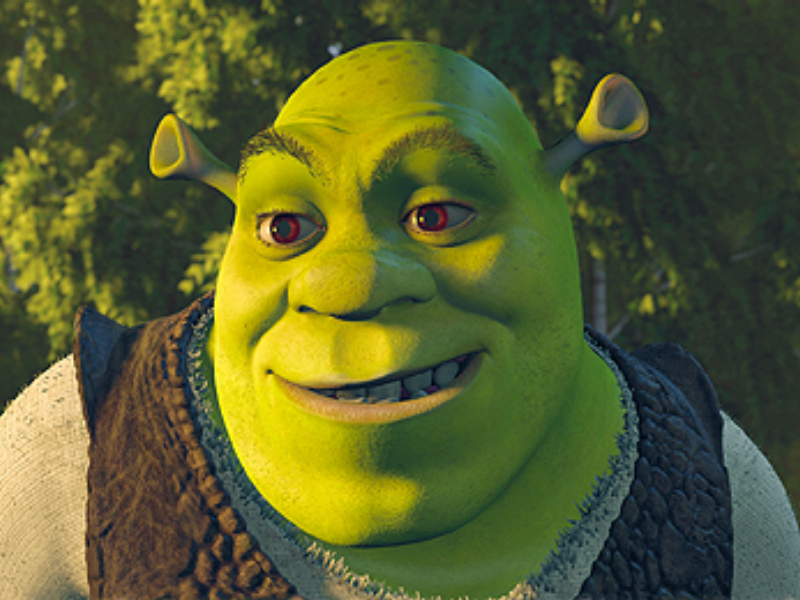
\includegraphics[width=4.7cm]{../images/shrek} &
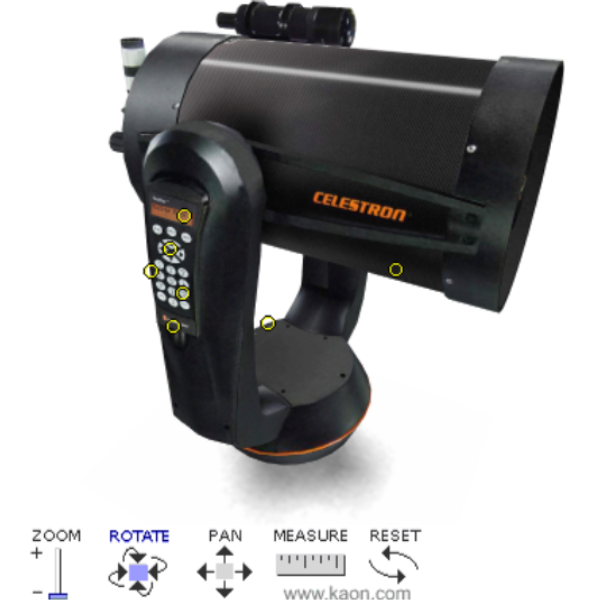
\includegraphics[width=3.5cm]{../images/kaon} &
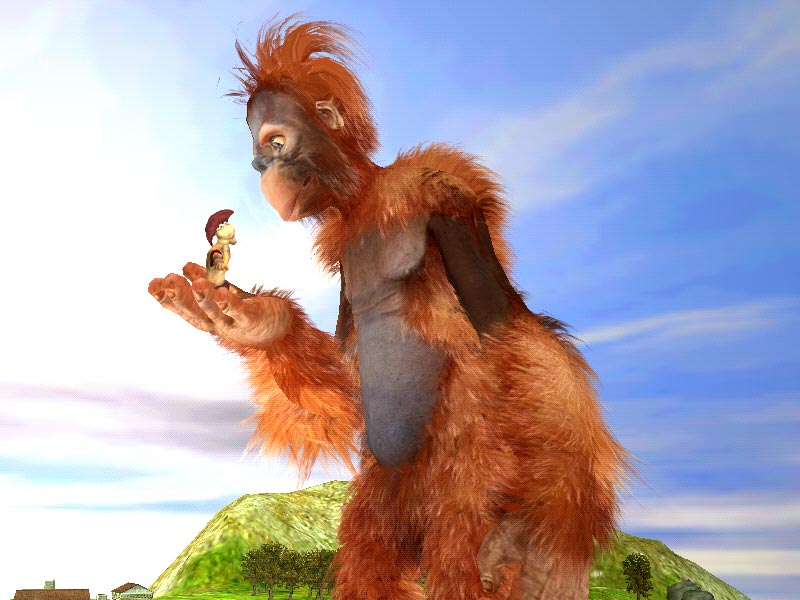
\includegraphics[width=4.7cm]{../images/black_white} \\
{\it (a)} & {\it (b)} & {\it (c)}
\end{tabular}
\caption[Uses of 3D Graphics]{\label{fig:3dgraphics} Uses of 3D Graphics. (a) Film: a still from {\it Shrek} from PDI/Dreamworks\cite{PDI}. (b) Online: 3D product visualisation by Kaon\cite{Kaon}. (c) Games: a screenshot from {\it Black \& White 2}, by Lionhead Studios\cite{Lionhead}.}
\end{center}
\end{figure}

\section{\label{sec:introduction:contentcreation}3D Content Creation}

The 3D content creation process however, has not kept pace with this explosion in visualisation capabilities. One of today's major challenges is to create models that have highly detailed, realistic surfaces, but can also be animated realistically. The process of creating realistic 3D content is still extremely time consuming, even for skilled artists. Therefore, in order to keep pace with the demand that the hardware and the public have for 3D content, we require new methods of content creation which are faster and more highly automated than traditional modelling techniques. We must also consider methods for efficient transport and delivery of this realistic content, as network bandwidth will always lag behind the capabilities of computer hardware to process such data.

Within the field of 3D content creation, one particular problem is the creation of accurate models of real-world objects. Such models can be created using one of two methods - either they can be created from scratch by an artist using a 3D modelling tool such as 3D Studio MAX or Maya, or alternatively, object scanning hardware can be used to capture the surface. 

The first method is wholly manual, extremely time-consuming, and requires a large amount of skill on the part of the content creator. The second method lends itself to automation, potentially reducing the skill and time required to create a realistic model. Advances in 3D sensor technology have provided an efficient way to capture photo-realistic 3D models of real objects. However, such reconstructed surface models are usually composed of a dense, unstructured polygonal mesh representing the surface detail of the object at the full resolution and accuracy of the sensor. As noted by \citet{Thalmann96}, such meshes are notoriously expensive to store, transmit, and render, and in particular are extremely awkward to animate. The goal of this research is to enable the creation of high-quality models based on captured surface data, that can also be animated efficiently \cite{Sun99}.

We discuss the state of the art for the problem of animating such dense surface data in Chapter \ref{sec:litreview}. In particular we discuss prior art in model capture and animation, focusing in particular on 3D capture systems, model representations, character animation, and compression of 3D data.

\section{\label{sec:introduction:layered}Layered Models}

\begin{figure}
\begin{center}
\begin{tabular}{cccc}
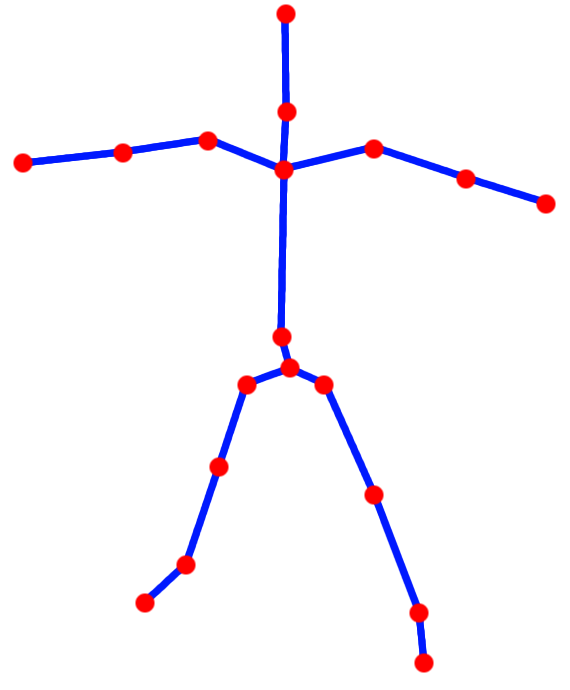
\includegraphics[width=4.4cm]{../images/skeleton_layer} &
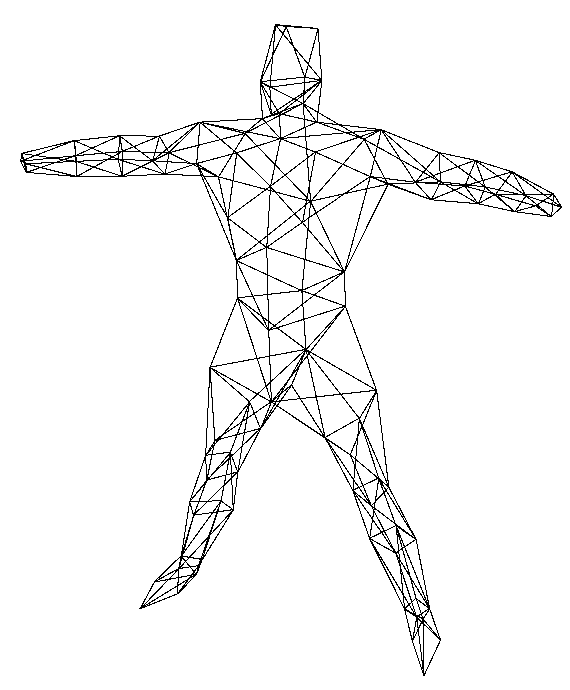
\includegraphics[width=4.4cm]{../images/control_layer} &
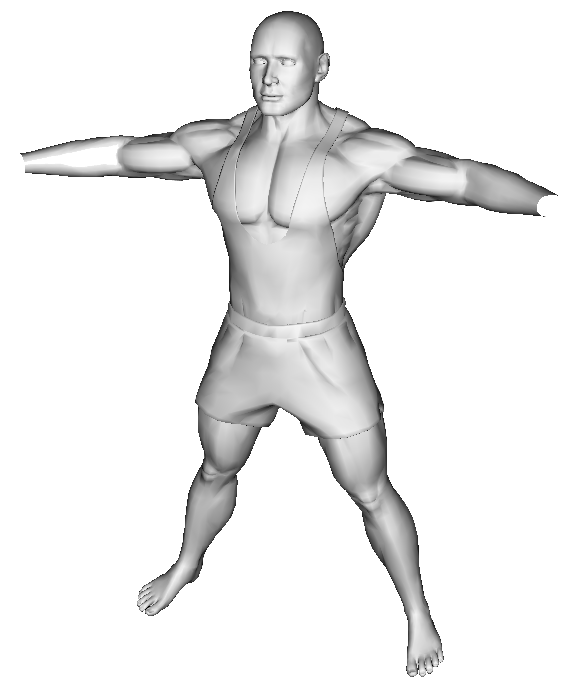
\includegraphics[width=4.4cm]{../images/detail_layer} \\
{\it(a)} & {\it(b)} & {\it(c)}
\end{tabular}
\caption[Layered Models]{\label{fig:layeredmodel} Layered Models (a) Skeleton Layer  (b) Control Layer  (c) Detail Layer}
\end{center}
\end{figure}

Typically, surface models reconstructed from captured data are composed of millions of polygons, and the articulation structure of the object is unknown. Animating such datasets directly is computationally expensive and it is difficult to achieve a realistic result. 

In order to solve this problem, we introduce methods for reconstructing {\it layered models} from captured data, which facilitate realistic animation. The model consists of a number of separate layers, each of which performs a different animation task; in particular, the layered model allows an animator to manipulate a low-resolution version of the model in real-time and render the full surface detail offline to achieve full quality output.

This approach provides a relatively fast and simple technique for building animated models from captured surface measurements. The resulting model gives an efficient, realistic animation of the detailed surface, while providing a low-resolution control structure for real-time interactive animation. The method can also be extended to allow many extra applications, such as variable level-of-detail rendering and model compression.

\subsection{\label{sec:introduction:layered:skeletal}Skeletal Animation}
\nomenclature{\bf Skeleton}{A hierarchical articulation structure, which can be used to drive animation of a detailed surface.}
The lowest layer in our system is a {\it skeleton layer} (see figure \ref{fig:layeredmodel}a). A hierarchical skeleton structure is fitted interactively to the mesh, and can then be animated using common animation techniques such as keyframing, inverse kinematics, physics-based models, or motion capture. The use of a skeleton layer greatly simplifies the process of animating the captured model, as the motion of the skeleton, which is easily defined, can be used to provide control of all the higher layers. In chapter {\ref{sec:skeletalanim}, we present a novel skeletal animation technique which requires minimal operator input during the creation phase, and we also present a complete implementation of this animation system in VRML.

\subsection{\label{sec:introduction:layered:control}The Control Layer}
\nomenclature{\bf Control Layer}{A mesh representation of an object containing a relatively low number of polygons.}
The middle layer is a low-resolution {\it control layer} (see figure \ref{fig:layeredmodel}b). Although the skeleton alone would be sufficient for motion control of the scanned data, it is too simple to be used as a representation of an object during animation design. For instance, a skeleton model would be unsuitable for collision detection or accurate targeting for inverse kinematics systems. On the other hand, the high-resolution model is prohibitively expensive to work with. Therefore it is desirable to introduce an intermediate layer. This control layer is a representation of the object with the same basic shape and topology as the captured data, but a much lower polygon count. This control layer can be a simplification of the captured data, a completely separate generic model, for instance a box-like model such as Discreet's Biped from 3D Studio MAX\cite{3DSMAX}, or a more complex structured model such as those available from Viewpoint\cite{Viewpoint}. This control layer is mapped to the skeleton layer, enabling its animation to be driven by movements of the skeleton structure. The process of mapping the control layer to the skeleton layer, and using this mapping to animate the control layer mesh based on skeletal motion is discussed in detail in chapter \ref{sec:skeletalanim}, as part of our discussion of skeletal animation. 

\subsection{\label{sec:introduction:layered:scandata}Animation of Dense Scanned Data}
\nomenclature{\bf Detail Layer}{A complex polygon mesh representing the surface of a scanned object at the maximum level of detail measured.}
The topmost layer in our model is the {\it detail layer} (shown in figure \ref{fig:layeredmodel}c). This layer is composed of the original high-resolution captured data, and is used in the final full-quality rendering stage of production, to reconstruct an accurate surface for the object. The detail layer is mapped to the control layer, allowing control layer animation to drive changes in the geometry of the detail layer. In chapter \ref{sec:scandata}, we present the mapping and animation methods which, when taken together with the aforementioned skeletal animation of the control layer, allow us to apply skeletal animation techniques to dense scanned surface data. 

\section{\label{sec:introduction:dispmaps}Displacement Maps}
\nomenclature{\bf Displacement Map}{A 2D image in which each pixel represents a displacement value for the surface of a control layer at the corresponding texture coordinate.}
\nomenclature{\bf Texture Map}{A coloured 2D image that is mapped onto a surface to represent details that are not present in the geometry of the surface.}
\begin{figure}
\begin{center}
\begin{tabular}{cc}
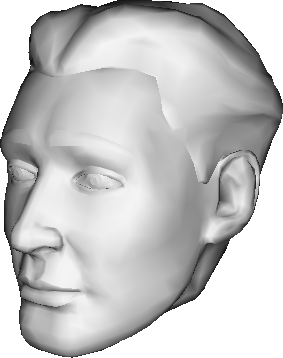
\includegraphics[height=5cm]{../images/cubehead_detail} &
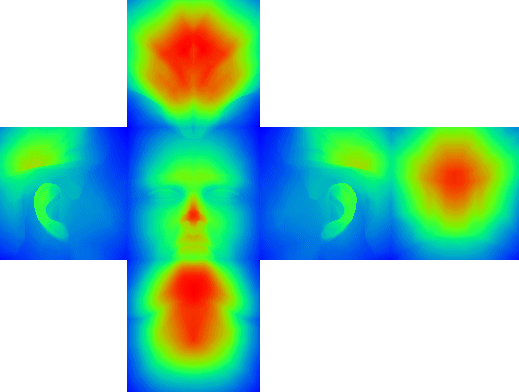
\includegraphics[height=5cm]{../images/cubehead_full} \\
{\it (a)} & {\it (b)}
\end{tabular}
\caption[Displacement Mapping]{\label{fig:dispmaps} Displacement Mapping. The detailed model shown in (a) can be represented as the displacement map shown in (b). The displacement map has been colourised to enhance the visibility of details. }
\end{center}
\end{figure}
The layered animation method described above allows us to animate dense datasets easily. However, it still requires animation and rendering of the full dataset, which may be too computationally expensive for anything but offline rendering. We therefore present an alternative representation of the detail layer using {\it displacement maps}. The detail layer is represented as a continuous 2D function across the surface of the control layer, which can be stored in an image form, similar to a texture mapped polygon mesh. An example is shown in figure \ref{fig:dispmaps}. This representation has a number of potential advantages, including variable level-of-detail rendering, simple editing, and geometry compression. The process of creating a displacement map for a detail layer is discussed in chapter \ref{sec:dispmapcreation}. Reconstruction and animation of displacement mapped models, as well as editing and compression, are discussed in chapter \ref{sec:dispmapanim}.

\section{\label{sec:introduction:whodidwhat}Division of Labour}

The techniques and algorithms discussed in this thesis were developed in conjunction with Adrian Hilton, Wei Sun, and Gordon Collins of the University of Surrey. In the areas where I did not carry out the majority of the work myself, it will be made clear in the text.

\section{\label{sec:introduction:publications}Publications}

As well as this thesis, the layered animation and displacement mapping methods have been presented in a number of published papers.

\begin{itemize}
\item{\bibentry{Sun99}}.
\item{\bibentry{Smith00}}.
\item{\bibentry{Sun00}}.
\item{\bibentry{Smith00a}}.
\item{\bibentry{Sun01}}.
\item{\bibentry{Starck03}}.
\end{itemize}

\chapter{\label{sec:litreview}The State of the Art}

In order to develop new methods to ease the model creation process, we must first understand the efforts that have already taken place in the field. We must understand the scanning and modelling process, and how models will be animated once they have been created. In this chapter, we will review current methods of model creation and animation, as well as related areas such as surface representation and compression. This is an area with a large commercial element, so we must understand not only academic research into these fields, but also commercially-available hardware and software systems. 

We start by examining systems for capturing detailed surface measurements from physical objects, and then review the possible representations in which this data can be stored. We are particularly interested in highly detailed surfaces, and therefore review a number of methods for representing such surfaces in an efficient manner, including methods of compressing this data. We also wish to animate the models that we will create, and so we end by reviewing current methods of mesh animation.

This review does not aim to be exhaustive, due to the wide range of material covered, but instead aims to highlight major approaches in order to provide an overview of the field.

\section{\label{sec:litreview:scanning}3D Scanning Systems}
In  this research, we wish to represent detailed models in an efficient manner. We must therefore discuss how such models are obtained. This can be done either by creating an object on a computer from scratch, using tools like 3D Studio MAX \cite{3DSMAX} or Maya \cite{Maya}, or it can begin with a physical object in the real world. In this case, a digitised model of the physical object must be created.

The first stage in any 3D scanning system is the capture of surface data from the physical object, the scanning or sensing phase \cite{Isdale98}. This involves using some form of hardware system to measure the surface of the object. Such systems fall into three main categories; tracking, imaging and range finding.

\subsection{\label{sec:litreview:scanning:tracking}Tracking}
Tracking systems typically capture data by positioning a probe on the surface of the object and capturing a single 3D point at a time. For instance, Coordinate Measuring Machines (CMMs) consist of a probe attached to a mechanical arm, which contains sensors that precisely measure the position of the probe when a point is captured. Other systems use different methods of tracking to provide greater freedom, such as electromagnetic and ultrasonic trackers. Such manual capture systems can be extremely time-consuming, as each point in the final model needs to be captured individually.

\subsection{\label{sec:litreview:scanning:imaging}Imaging}
Imaging systems take a number of 2D images of an object, normally from different angles, which are then processed to calculate 3D surface data. Imaging systems range from systems that generate point clouds by calculating range measurements, to systems that generate models directly by extracting feature points from the image data. Other systems use the silhouette of the object to create a volumetric model which can then be converted into a polygonal representation. Medical scanners also come under the heading of imaging systems, using sensors such as MRI, CT and so on \cite{Short02}.

\subsection{\label{sec:litreview:scanning:range}Range Finding}
Range finding systems generally produce a 2D array of distance measurements known as a {\it range image}, which can be easily converted into a mesh. The most common type of range finding systems are laser scanners, which project a laser stripe onto the surface being scanned, and capture the shape of the stripe through a camera positioned at an angle to the laser. This can be converted into a set of distance measurements, in a process known as {\it optical triangulation}. Some systems are also capable of capturing texture information from objects, which can then be mapped onto the generated models. 

A popular technique is to combine a tracking system and a range finder. Systems of this kind include 3D Scanner's ModelMaker \cite{3DScanners}, which uses a CMM arm with an attached laser scanner, and the Polhemus HLS \cite{Polhemus}, which uses Polhemus' magnetic tracking system with a laser scanner. This type of system allows the scanner to be moved freely around an object, while capturing position and orientation information for the scanner itself. Some scanners, such as those from \citet{Cyberware}, move a laser scanner around the object automatically, but this requires a large working area and complex machinery. 

Such systems generally produce very dense, unstructured surface data, which is very difficult to work with. In order to be usable, this data must be processed into a more easily manipulated format.

\section{\label{sec:litreview:surfaces}Surface Representations}
\begin{figure}
\begin{center}
\begin{tabular}{ccc}
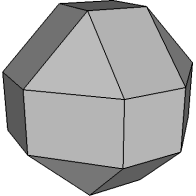
\includegraphics[width=3.5cm]{../images/polymesh} &
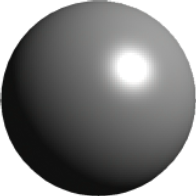
\includegraphics[width=3.5cm]{../images/quadric} &
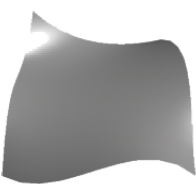
\includegraphics[width=3.5cm]{../images/nurbs} \\
{\it(a)} & {\it(b)} & {\it(c)}
\end{tabular}
\caption[Surface Representations]{\label{fig:surfaces} Surface Representations. (a) Polygonal Mesh. (b) Quadric Ellipsoid. (c) NURBS Surface.}
\end{center}
\end{figure}
In order to represent an object in a computer, we must store data about its surface in some form or another. There are a number of possible surface representations we can choose from, each with their own advantages and disadvantages.

\subsection{\label{sec:litreview:surfaces:polygon}Polygonal Surfaces}

Polygonal models represent a surface using a set of planar polygons, usually triangles or quadrilaterals, as shown in figure \ref{fig:surfaces}a. These surfaces are the the dominant form of representation in 3D graphics, particularly at the consumer level, where much effort has been expended to create hardware that can render polygonal models as fast as possible. However, with the desire for increasingly realistic graphics, their limitations have become clear.

Polygonal models can approximate surfaces of arbitrary complexity, but as they are piecewise linear, they cannot truly represent curved surfaces \cite{Besl94}. Even a close approximation to the surface would require a large number of polygons.

\subsection{\label{sec:litreview:surfaces:smooth}Smooth Surfaces}

Many surfaces that we wish to model are curved and, as noted above, accurately representing a curved surface with a polygonal model would require a large number of polygons. Instead, we can use {\it smooth} surfaces to represent such models. Unlike polygonal models, smooth surfaces are not piecewise linear, so are capable of representing curved surfaces efficiently.

\subsubsection{\label{sec:litreview:surfaces:smooth:polynomial}Polynomial Surfaces}

Most 3D rendering packages include support for {\it polynomial} surfaces, which result from the evaluation of a polynomial function in terms of spatial coordinates. The order of the polynomial defines the smoothness of the surface. First-order polynomials define planar C0 surfaces, and second-order polynomials define C1 {\it quadric} surfaces such as ellipsoids and paraboloids (see figure \ref{fig:surfaces}b). Cubic and quartic surfaces are also common. This form of representation is limited to representing the surfaces that can be represented by a polynomial equations, however, and cannot represent surfaces of arbitrary geometry and topology.

\subsubsection{\label{sec:litreview:surfaces:smooth:curved}Curved Surface Patches}

Curved surface patches are a generalisation of smooth 2D curves to three dimensions. The surface is generally a quadrilateral patch whose geometry is defined by a number of control points. Due to the fact that curved surfaces can only represent quadrilateral patches, modelling of complex objects requires the use of multiple patches, which must be held together, or {\it stitched}, so that cracks do not appear during animation.

Two dimensional smooth curves use a polynomial function to define the shape of the curve. The coefficients of the polynomial are the {\it control points} of the curve. Two of the more popular types of curve are {\it Bezier} and {\it B-Spline} curves, both defined by a cubic polynomial. In a Bezier curve, two control points define endpoints, while another two control the shape of the curve between the points. The cubic B-Spline is a generalisation of the Bezier curve, and defines the curve its two innermost control points, using the other two to control endpoint gradients. Using B-Splines, a curve with an arbitrary number of control points can be specified by stitching B-Spline curve segments together. If the control points for one B-Spline overlap the control points for the next, the two will be C2 continuous at the join.

\citet{Forsey88} describe an extension to B-Spline surfaces, the {\it Hierarchical B-Spline patch}. These patches can be refined as required (for instance in areas of high surface detail) by adding extra control points, creating a higher-order surface in the local area.

\subsubsection{\label{sec:litreview:surfaces:smooth:nurbs}NURBS Patches}

Non-Uniform Rational B-Splines (NURBS), illustrated in figure \ref{fig:surfaces}c, are a general form of B-Spline, and are now a popular representation for curves and surfaces. They have two properties over normal B-Splines that make them particularly popular. Firstly, both NURBS and B-Splines can be subjected to affine transformations without distortion. However, perspective transformations are not affine, and B-Splines do not appear correctly under perspective viewing. NURBS, however, do not suffer from this, and appear as intended even after non-affine transformation, a vital property for 3D graphics. Secondly, quadric surfaces can only be approximated by standard B-Splines, but can be shown to be a special case of NURBS.

\subsubsection{\label{sec:litreview:surfaces:smooth:implicit}Implicit Surfaces}

An implicit surface is not defined by explicit evaluation of an equation, or by a set of 3D points, but as the set of solutions to a function of the form $f(x,y,z) = a$. The surface itself is a contour or {\it isosurface} in the 3D scalar field defined by the function, and upon which the result of the equation is some constant value $a$ (normally 0). For rendering purposes, implicit surfaces can be {\it tiled}, or converted into a polygonal representation \cite{Ning93}.

\subsubsection{\label{sec:litreview:surfaces:smooth:subdivision}Subdivision Surfaces}
Recently, {\it subdivision} surfaces have gained popularity, and have been incorporated into a number of rendering packages. Subdivision surfaces bridge the gap between polygonal and smooth surfaces, by using an arbitrary polygonal mesh to define a parametric surface. The subdivision surface is created by repeated application of a subdivision algorithm to the polygonal control mesh. The limit of this process defines a smooth spline surface. There are a number of different types of subdivision surface, each with its own subdivision algorithm and restrictions on control mesh structure. The major types are Doo-Sabin \cite{Doo78}, Catmull-Clark \cite{Catmull78}, Loop \cite{Loop94} and Butterfly \cite{Dyn90} surfaces. 

\begin{figure}
\begin{center}
\begin{tabular}{cccc}
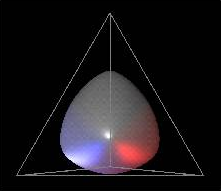
\includegraphics[width=3.18cm]{../images/tetra_doosabin} &
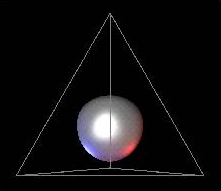
\includegraphics[width=3.18cm]{../images/tetra_catmullclark} &
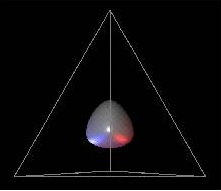
\includegraphics[width=3.18cm]{../images/tetra_loop} &
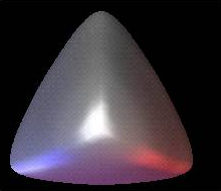
\includegraphics[width=3.18cm]{../images/tetra_butterfly} \\
{\it(a)} & {\it(b)} & {\it(c)}  & {\it(d)}
\end{tabular}
\caption[Subdivision Surfaces]{\label{fig:subdivision} Subdivision Surfaces. (a) Doo-Sabin subdivision. (b) Catmull-Clark subdivision. (c) Loop subdivision. (c) Butterfly subdivision. Images taken from \cite{Zorin99}.}
\end{center}
\end{figure}

Doo-Sabin subdivision, shown in figure \ref{fig:subdivision}a, is a {\it dual} subdivision method based on quadratic uniform B-Spline surfaces. Each level of subdivision divides each vertex into {\it n} new vertices, where {\it n} is the number of faces adjacent to the vertex. The new positions of the new vertices are calculated as the average of the original vertex, the centroid of the face, and the midpoints of the two edges adjacent to the face and the original vertex.

Catmull-Clark surfaces (shown in figure \ref{fig:subdivision}b) are based on the subdivision of cubic uniform B-Spline surfaces, and create a three kinds of new vertices at each subdivision step. New points are added in the centre of the faces of the control mesh, and at the midpoints of control mesh edges. The control mesh vertices are also affected by the subdivision.

Both of the above subdivision schemes use control meshes of arbitrary topology. Loop subdivision (see figure \ref{fig:subdivision}c) however, uses control meshes composed only of triangles. At each level, each triangular face is divided into four smaller faces, and smoothed based on the subdivision of quartic uniform box splines.

All of the above schemes use an {\it approximating} subdivision scheme, in which the original control vertices do not necessarily lie on the limit surface. Butterfly subdivision, illustrated in figure \ref{fig:subdivision}d, is an {\it interpolating} scheme, in which original control points are preserved on the limit surface. Like Loop, Butterfly subdivision works on a control mesh composed of triangular faces.

Subdivision surfaces can be extended to allow sharp edges by constraining the subdivision routine. \citet{Hoppe94a} proposed such a method for Loop surfaces, and \citet{DeRose98} have developed a similar method for Catmull-Clark surfaces.

\subsection{\label{sec:litreview:surfaces:detail}Representation of Surface Detail}
\begin{figure}
\begin{center}
\begin{tabular}{ccc}
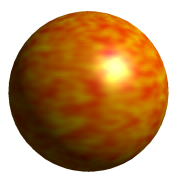
\includegraphics[width=3.5cm]{../images/sphere_texmap} &
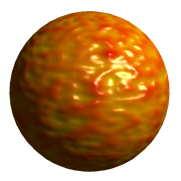
\includegraphics[width=3.5cm]{../images/sphere_bumpmap} &
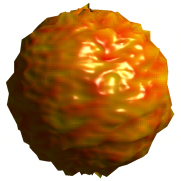
\includegraphics[width=3.5cm]{../images/sphere_dispmap} \\
{\it (a)} & {\it (b)} & {\it (c)} \\
\end{tabular}
\caption[Surface Detail]{\label{fig:surfacedetail} Surface Detail. (a) Texture mapping. (b) Bump mapping. (c) Displacement mapping.}
\end{center}
\end{figure}
A polygonal or smooth surface can represent the general shape of an object efficiently, but realistic objects possess fine surface details, such as wrinkles in skin. Unless the model is extremely detailed, these are impossible to represent, as well as difficult to edit. A polygonal model would require a very large number of faces to represent small surface details, and a smooth surface would need either a large number of patches or a very high order polynomial. Both of these will increase rendering time, and therefore prohibit interactive animation. A number of techniques have therefore been developed to create the illusion of a detailed surface without requiring complex geometry.

The simplest of these is {\it texture mapping}, shown in figure \ref{fig:surfacedetail}a, where a 2D image of the surface of the real object is mapped onto the surface of the model. This gives the appearance of surface detail, but has a limitation in that the texture will not change under different lighting conditions. The underlying geometry of the surface is also visible when examined closely.

A more realistic appearance can be created by {\it bump mapping}, proposed by \citet{Blinn78}, which applies details during shading of the surface. A bump map is a texture used to perturb the normal of the surface during shading. This changes the lighting on the surface, making it appear as if the surface detail is actually present. The surface itself is still the original shape, as can be seen from the object's silhouette.

The most realistic results are obtained using {\it displacement mapping}, originally proposed by \citet{Cook84}. Displacement mapping is a step beyond bump and texture mapping in that it actually perturbs the geometry of the surface it is applied to. A displacement map is generally an image where each pixel encodes an offset along the surface normal, which is mapped onto the surface. During rendering, a new surface is created which includes all of the surface detail from the displacement map. As this approach actually changes the surface geometry, the result is indistinguishable from a very detailed mesh. However, displacement maps are currently very expensive to compute, and while they have been used in film production for a reasonable length of time, until recently they have been of limited use for real-time applications. However, the power of consumer graphics cards is now such that current graphics APIs include displacement map support \cite{DirectX9}, and hardware support will not be far behind. The use of displacement maps for modelling is discussed further in section \ref{sec:litreview:modeling:detail}.

\section{\label{sec:litreview:reconstruction}Surface Reconstruction}

After surface measurements of an object have been taken, we must convert these measurements into a form that we can use, such as those mentioned above in section \ref{sec:litreview:surfaces}.

In many cases, the surface data will be in the form of a set of range images that must be fused into a single surface. There are two main problems involved in merging multiple range images \cite{Illingworth98}. The first is the problem of {\it registration}, which involves positioning the range images correctly relative to each other. When multiple range images are taken without information on the sensor position for each one, this is a major problem \cite{Besl92}. However, the combination tracker/scanner systems avoid this problem, as the scanner position is always known. In these cases, we only have to solve the second problem, how to fuse the multiple range images together into a single surface.

Early approaches to this problem concentrated on fitting deformed polynomial surfaces such as planes and spheroids to the range data. These methods have their obvious limitations, being confined to the reconstruction of surfaces with the same topology as the polynomial surface.

\subsection{\label{sec:litreview:reconstruction:fusion}Mesh Fusion}

An early attempt at a solution using triangulated meshes was proposed by \citet{Turk94}, who developed a method that triangulated individual range images into a set of polygon meshes, which were then stitched or {\it zippered} together. However, this approach produces a large number of small thin triangles along the zippered edges, and has been shown to be error prone.

\citet{Rutishauser94} describe an alternative method for merging a pair of triangulated range images, by performing a mutual approximation of the two meshes, using an explicit error function which fades between the two surfaces. A re-triangulation is then performed to merge the two meshes into one. However, this algorithm can break down in areas of high surface curvature.

\subsection{\label{sec:litreview:reconstruction:implicit}Implicit Approaches}

A method to create surfaces from disorganised point sets was proposed by \citet{Hoppe92}, using an implicit surface based approach. An implicit surface is built from the range data, which is then converted into a polygonal representation. This method works well for simple objects, but can be very computationally expensive for models with a large number of points.

\citet{Curless96} describe a related method which stores the implicit surface in a volumetric model, a discrete 3D grid made up of semidisjoint cells called {\it voxels}. The surface is encoded implicitly in the volumetric model by calculating the signed distance from the triangulated mesh for each voxel in the volume. As new range images are added, the complete surface is built up as an isosurface inside the volumetric model, which is then polygonised. 

\citet{Hilton96b} suggest a more robust approach, which only calculates the value of the signed distance function at precise positions as required by the polygonisation algorithm as it executes. This means that the signed distance function is no longer discrete, but continuous, allowing more efficient and accurate reconstruction of the isosurface, even in areas of high curvature and thin sections.

All implicit surface methods require the resulting implicit surface to be converted to a polygonal representation. The most popular approach to this problem is the Marching Cubes algorithm proposed by \citet{Lorensen87}. This algorithm partitions the volume occupied by the model into voxels. The value of the implicit function is then evaluated at the cell vertices, which indicates if a cell is {\it transverse} or crosses the isosurface. If a cell edge has a positive vertex at one end and a negative vertex at the other, the surface must cross that edge. Once all the crossing points are found, a set of polygons can be constructed inside the cell, which correspond to the shape of the surface inside that cell.

Such spatial partitioning methods of surface tiling have a number of drawbacks, including the fact that the resulting triangulation is extremely irregular. This is a common issue with all 3D capture systems, which generally produce highly unstructured meshes, that are unsuitable for animation.

\section{\label{sec:litreview:modeling}Model Creation}

There is no standard method of creating 3D models suitable for animation, especially from scanned data. Many models are created from scratch using software tools, with no reference to real objects, but this can be very time consuming, especially for detailed models. Alternatively, a physical model can be digitised as described above. The problem with this approach is that the dense polygon meshes created by such scanning systems are inappropriate for use in animation. The models have far too many polygons to be usable in interactive modelling packages, and the meshes are unstructured, in that that the polygon edges do not follow the natural curvature of the surface. The process of animating scanned objects therefore involves the reduction and restructuring of this dense data.
 
\subsection{\label{sec:litreview:modeling:techniques}Modelling Techniques}

One approach is to create a polygon mesh directly by using a touch probe scanner or CMM. Particular points (corresponding to the vertices desired in the final model) on the surface of the object are measured, and the mesh is reconstructed directly from the scanned points. This allows rapid construction of a 3D model, but the topology of the mesh must be designed by hand before scanning. This is the approach taken by \citet{Viewpoint}, a major supplier of 3D models for animation.

\begin{figure}
\begin{center}
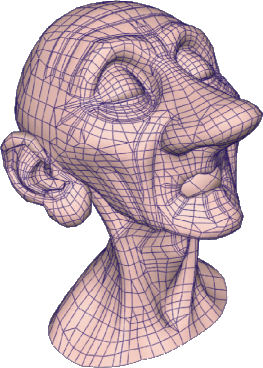
\includegraphics[height=5cm]{../images/geri_control}
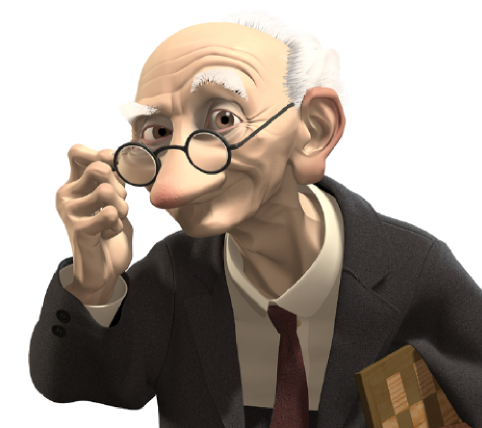
\includegraphics[height=5cm]{../images/geri2}
\caption[Pixar's Geri]{\label{fig:geri}Pixar's Geri, from their short film {\it Geri's Game}. A clay model of the head is digitised at particular points to obtain control points for a Catmull-Clark subdivision surface. Images taken from \cite{DeRose98}.}
\end{center}
\end{figure}
\citet{Pixar} have had some success in modelling surfaces using Catmull-Clark subdivision surfaces \cite{DeRose98}. For their short film {\it Geri's Game}, they created the head, hands and clothing of the main character by sculpting a clay model and capturing surface points with a CMM. These scanned points were then used as control points for the subdivision surface, illustrated in figure \ref{fig:geri}.

Alternatively, the dense scanned data can be retriangulated by hand. This allows a highly structured mesh to be constructed, but is very labour-intensive and can take many days of skilled work to remodel a complex surface. Nevertheless, this is the approach that is currently used by many animation houses, including \citet{Hensons}.

Animation systems that require an extremely accurate appearance, particularly for modelling realistic characters, utilise a highly layered anatomical approach. A skeleton model is built, and a muscle layer added on top. The densely scanned skin layer is mapped on top of this muscle layer, possibly with an extra layer in between to simulate body fat. Needless to say, this approach requires a great deal of skill and specialist knowledge to model, and a great deal of processing time to render and animate. The results, however, can be highly realistic.

\subsection{\label{sec:litreview:modeling:detail}Displacement Maps}

Fitting a polygonal or smooth surface to scanned data can represent the general shape of a model well, but fine surface details can be lost, as the surface cannot represent them at a high enough level of detail and remain efficient. However, a number of approaches have been suggested to store this residual detail in a displacement map, allowing an efficient yet detailed surface to be created. Much research has focused on hardware rendering of these representations (\cite{Gumhold99a}, \cite{Doggett00}), making it likely that the use of displacement maps will become more commonplace in the near future.

\citet{Krishnamurthy96} describe a method in which an object is scanned and converted into a dense polygon mesh. They then split this mesh into quadrilateral sections by manually drawing curves across the surface, reasoning that an automatic process will not create a surface suitable for animation. A B-Spline patch is then fitted to each section, creating a smooth representation of the model. The differences between this surface and the original polygon mesh are then encoded in a vector-valued displacement map for each patch, storing the fine details.

\citet{Lee00} define a similar method of representing complex datasets using displaced subdivision surfaces. A simplified version of a dense detailed mesh is generated using the MAPS algorithm \cite{Lee99}, which defines a control mesh for a Loop subdivision surface which approximates the scan data. At a number of sample points on the limit surface, a ray is cast along the surface normal, and an intersection calculated with the detailed polygonal surface. The distance between the two surfaces is then stored in a scalar-valued displacement map. Reconstruction is performed by calculating the the Loop subdivision of the control mesh, after which the stored displacement values are added to the new vertex positions. This representation allows fine surface detail to be encoded as a scalar field, making this a much more compact representation than the previous method. \citet{Jeong01} describe a method for building displaced subdivision surfaces directly from scanned surface data.

Lee's method is similar to that presented in this thesis, except that he uses a smooth base domain for his displacement maps, whereas we use a polygonal mesh surface. Lee also uses a low-to-high mapping to create his displacement maps, whereas we use a high-to-low mapping based on our intermediate detail layer representation. Both methods were developed concurrently, and we present our work as an alternative to this approach. A detailed comparison of the two methods is presented in section \ref{sec:conclusion:dispsubdiv}.

Such displacement map approaches store the fine details of a surface in an image format. \citet{Gu02} define a method which represents the complete mesh surface in this form, known as a {\it Geometry Image}. The dense dataset is first unwrapped automatically onto a 2D image plane. At each point in the image, the 3D position of the corresponding point on the dense surface is stored as a 3D vector, with the three components of the vector being stored in the three colour planes of the image. Normal images can also be created, which store the surface normal at each point in a similar fashion. This approach has the rather unique property that the geometry of the surface is stored in exactly the same manner as other surface features, such as texture and colour information.

\citet{Botsch03} describe a method related to displacement mapping that represents surfaces using {\it displacement volumes}, instead of using individual vectors for surface displacement. Rather than keeping the displacement between the base domain and the detailed surface the same, their approach preserves the volume of the surface under animation, giving a more realistic appearance in some circumstances.

\subsection{\label{sec:litreview:modeling:compression}Mesh Compression Techniques}

As well as simplifying complex datasets for animation purposes, it is sometimes useful to be able to keep those datasets in their original form, but still store and transmit them in an efficient manner. Progressive transmission of large datasets is also desirable, as a simplified version of the surface can be displayed quickly, followed by more complex versions \cite{King01}.

The field of mesh compression is young, and evolving rapidly. Most research falls into one of three categories. First, mesh-based approaches concentrate on the compression of geometric or topological data, by splitting the mesh surface into sections or strips. Examples include Topological Surgery by \citet{Taubin98}, which is used in MPEG-4, and the Edgebreaker method by \citet{Rossignac99}.

Alternatively, progressive approaches concentrate on reducing complex meshes into very simple ones, and then rebuilding the detailed surface one vertex at a time. \citet{Hoppe96} proposed an algorithm which simplifies mesh geometry through a series of edge collapses. This creates a low-resolution mesh which can be rebuilt one vertex at a time by reversing the edge collapse operation. \citet{Guskov00} define a similar method, which converts a retriangulated mesh into a simple base domain and a single floating-point coefficient per detail vertex. This floating point number represents a displacement from the base domain, and again allows a mesh to be rebuilt a single vertex at a time. The current state of the art in mesh compression, however, is proposed by \citet{Khodakovsky00}. Their method uses MAPS \cite{Lee98} to convert a dense mesh into a series of semi-regular approximations at different levels of detail. The refinement parameters between these approximation levels are then compressed with a wavelet-based encoding method, giving very high levels of lossy compression.

Increasingly, however, research is being carried out into the use of image methods for mesh compression. By representing meshes in an image-based form, either as displacement maps (\cite{Lee00}, \cite{Krishnamurthy96}), or as geometry images \cite{Gu02}, years of research into image compression can be applied to the efficient storage of large meshes. Such approaches are showing promise, but more research is yet to be done.

\subsection{\label{sec:litreview:modeling:software}Commercial Software}

There are a number of commercial software packages than incorporate some of the modelling techniques described above. 

{\it Remesh}, from \citet{3DScanners}, takes the approach of trying to ease the process of creating a structured polygon mesh from scan data. This would normally involve a large amount of manual joining of data points, as mentioned above, but Remesh allows the modeller to create a structured mesh from the a triangulated version of the original scan data without joining data points by hand. The modeller can draw {\it polylines} across the mesh, which are linked to define quadrilateral or triangular patches which are then subdivided to the desired resolution. This approach is described in more detail in section \ref{sec:scandata:creation:control:interactive}.

{\it Paraform} \cite{Paraform} implements the B-Spline patch modelling approach proposed by \citet{Krishnamurthy96}, described above. Geomagic {\it Shape} \cite{Geomagic} and Cyberware's {\it CySlice} \cite{Cyberware} create a similar representations based on NURBS patches. None of these packages deal with the animation of such models, however. They simply create a static mesh from the scan data, which can then be animated in a standard modelling package, such as 3D Studio MAX \cite{3DSMAX} or Maya \cite{Maya}.

\section{\label{sec:litreview:animation}Animation Techniques}
One of the most important applications for models built from scanned data  is the creation of models that can be animated, for use in special effects or games. The ability to scan rigid objects is useful, but ideally, we want to be able to create models that are non rigid, and that can move and bend. In short, we should be able to easily create {\it deformable} models.

\subsection{\label{sec:litreview:animation:skeleton}Articulation Structures}
\nomenclature{\bf Segment}{A rigid link between joints in a skeleton structure, for instance representing a bone in a human body.}
\nomenclature{\bf Joint}{A node in a skeleton structure, which can be rotated or transformed to provide control over the pose of the skeleton. }
\nomenclature{\bf End Effector}{A node in a skeleton structure which represents the end of the hierarchy, normally corresponding to feet, fingertips, and so on. }
\begin{figure}
\begin{center}
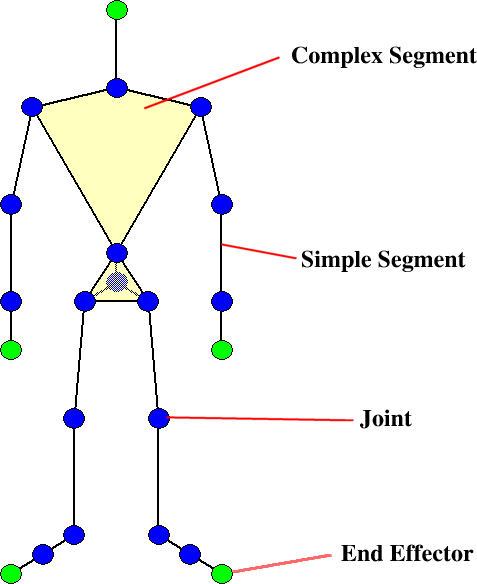
\includegraphics[height=7cm]{../images/skeleton_nosites}
\caption[Skeleton Structure]{\label{fig:skeleton} Skeleton Structure. A skeleton consists of a set of joints connected by rigid segment links.}
\end{center}
\end{figure}
Keyframing techniques are often used for model animation, but these can only represent a limited set of pre-calculated motions for a surface. In cases where arbitrary motions are required, {\it skeletal animation} is used. This uses a flexible articulation structure to drive motions of a surface or skin layer. A skeleton structure consists of a hierarchical series of {\it joints}, which are connected together by rigid links known as bones or {\it segments}, as shown in figure \ref{fig:skeleton}.

Skeletal animation is normally driven by joint rotations, in which a rotation is applied to each joint and its children. For instance, if a shoulder joint of a skeleton is rotated, the entire arm below that point rotates with it. Each joint rotation is applied incrementally, so the position of an individual segment will be defined by the rotations of all of the joints above it in the hierarchy. Rotation data for joint animation can be obtained in a number of ways, from manual location, through inverse kinematics systems (in which the modeller simply positions an {\it end effector}, for instance a foot, and the required joint rotations are calculated automatically), to motion capture systems that record the real-world movements of a human subject.

As well as the skeleton structure itself, the surface of a deformable model must be affected by transformations of the various joints. This is carried out by defining a method of attaching the surface to the skeleton, by associating parts of the surface with the skeleton in some way. The surface then deforms as the skeleton is moved. The most common methods of performing this association and deformation are described below.

\subsection{\label{sec:litreview:animation:geometric}Geometric Methods}

The first class of deformation techniques we will cover are geometric approaches. These type of methods have the advantage that the skin layer is operated on only by simple geometric transformations, as opposed to complex physical or anatomical simulations. This makes them comparatively cheap to calculate, and hence more appropriate for real-time applications. 

\subsubsection{\label{sec:litreview:animation:geometric:ssd}Skeletal Subspace Deformation}

The simplest method of deforming a skin model with a skeleton is to use vertex blending, or {\it Skeletal Subspace Deformation} \cite{Akenine02}. This technique has never been officially published, but related methods have been presented by \citet{Komatsu88}, and \citet{Magnenat-Thalmann88}. The technique is also used in many commercial animation packages.

\begin{figure}
\begin{center}
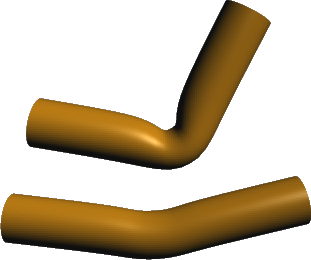
\includegraphics[width=7cm]{../images/bend}
\caption[Skeletal Subspace Deformation]{\label{fig:ssd} Skeletal Subspace Deformation. Simple deformation techniques suffer from collapse around joints, as well as during twisting.}
\end{center}
\end{figure}

SSD methods simply assign each vertex in a skin layer to one or more of the skeleton segments, along with a weight for each segment. The deformed position of the vertex is the weighted average of the original position after application of the transformation for each segment. This method can give realistic results, but can require much user interaction to define the vertex weights. It can also be unpredictable, and not all deformations can be represented in this fashion. Classic SSD problems include thinning around joints (shown in figure \ref{fig:ssd}), and the complete collapse of geometry under segment-aligned rotations.

\citet{Lewis00} describe a method which uses aspects of both keyframed and SSD animation. They define a set of poses for a surface, with user-defined geometry for each. Skeletal animation can then be applied, and the deformed surface is generated by shape interpolation between these key poses.

\subsubsection{\label{sec:litreview:animation:geometric:ffd}Free-Form Deformations}
Free-Form Deformation (FFD), proposed by \citet{Sederberg86}, is a method of deforming arbitrary objects. The object to be deformed is embedded in an FFD block, which is in fact a tricubic Bezier hyperpatch, an extension to three dimensions of the spline patches described in section \ref{sec:litreview:surfaces:smooth:curved}. In order to deform the surface, the hyperpatch control points are moved, thus changing the geometry of the hyperpatch and the object within it.

The FFD method has been extended by \citet{Coquillart90} to allow arbitrarily shaped FFD spaces to be created by combining a number of FFD lattices, a technique known as Extended Free-Form Deformation (EFFD). \citet{MacCracken96} further extend FFD to allow lattices of arbitrary topology.

\citet{Chadwick89} present an effective method of using FFDs for character animation, known as {\it Critter}. This system represents a deformable character as three layers; an articulated skeleton structure, a muscle layer (represented as a set of FFD blocks), and a skin layer, which is deformed by the FFD muscle layer. The muscle layer is constructed by placing an FFD block around each joint (called a {\it flexor}), and also one along each segment (called a {\it tendon}). The control points within each FFD block are also controlled by movements of the joints. Flexors are scaled orthogonally to the segment to simulate muscle inflation, while the faces of the tendons are rotated according to the rotation of closest joint. The faces of the FFD blocks are held together, so that when a joint bends, both the flexor and tendon blocks are affected.

\subsubsection{\label{sec:litreview:animation:geometric:bspline}Hierarchical B-Spline Models}
\citet{Forsey91} describes a method of constructing articulated characters using a hierarchical B-Spline representation. Control points for a set of B-Spline patches are attached to the segments of the skeleton, so that the smooth surface follows the movements of the joints. This is enough for gross movement of the surface, but detailed movements around the joints cannot be represented in this way. Therefore, the area around the joint is split into a number of subsegments, between which the rotation angle is divided up, giving a smoother joint in the skeleton. Extra control points can then be added to these, giving a smoother surface in joint regions.

\subsubsection{\label{sec:litreview:animation:geometric:metaballs}Metaballs}
\citet{Shen95} describe a method of modelling shapes using {\it metaballs}, which are fixed to the a skeleton to build up the deformable surface, simulating the appearance of muscles and so on. There is no precise relationship between metaballs and real muscles, however, making the modelling process completely subjective on the part of the modeller. The parameters of the metaballs, such as major and minor axes, are controlled by joint angles, so that the metaballs change shape as the skeleton moves. After deformation, the implicit surface of the combined metaballs is converted into a polygonal representation for display. At regular intervals along the segments of the skeleton, rays are cast orthogonally from the segment to the surface of the metaball body. The positions of the intersections with the surface become the vertices of the polygonal model. The polygonal model is therefore structured in contours, with a consistent number of vertices around each contour. 

This approach, though it produces realistic results, is computationally expensive, as the skin layer is recalculated completely every time the body is moved. \citet{Thalmann96} therefore propose an improved method, in which the polygonal surface of the model is generated only once after modelling, and all deformation is performed by rotating the contours of the polygonal model according to joint movements. This deformation method is fast enough for realtime calculation, and has been used to implement surface deformation in VRML by \citet{Babski99}.

\subsection{\label{sec:litreview:animation:physics}Anatomical and Physical Methods}
If highly realistic results are required, more complex anatomical or physical deformation techniques can be used. Physical methods of character animation involve some aspect of physics simulation, often a simple spring-based model. Anatomical methods construct a model that has several highly realistic layers, such as multiple muscles, fat and skin layers, and as such are almost always too expensive for realtime animation. Also, such models are very complex to build, and require the modeller to specify multiple weighting parameters dependent on the muscle or skin area being modelled. This is a very difficult process, and is not suited to rapid construction of models.

\subsubsection{\label{sec:litreview:animation:physics:layered}Layered Deformable Bodies}
\citet{Gascuel91} propose a method that uses three layers to construct a deformable model. The bottom layer is a normal skeleton structure, to which a physical spring simulation layer is attached. Springs are attached to the skeleton at one end, allowing the other end to move freely along the axis of the spring. Extensions of springs are propagated to other nearby springs, so that deformations are consistent within a small area. The free end of the spring is used as a control point for a B-Spline based skin layer. This approach is simple enough to compute in a reasonable time. The springs also handle collisions between body parts, so that realistic deformations around the inside of joints are obtained without self-intersection of the surface.

\subsubsection{\label{sec:litreview:animation:physics:anatomical}Anatomical Modelling}
A method for body modelling based on anatomical principles is proposed by \citet{Nedel98}. Their models consist of a large number of physically accurate muscles attached to accurate points on a skeleton model. Needless to say, the modelling effort required to create this kind of model is very large. The models are, however, based in reality, so the modelling process is not as subjective as for the metaball method described above. Upon movement of the skeleton, the muscles deform in a physically accurate way. The skin model is then generated after each movement in the same way as Shen's method for metaball modelling, by casting rays from the segments out to the surface of the muscles and generating contours for a polygonal model.

\subsubsection{\label{sec:litreview:animation:physics:leman}LEMAN}
The LEMAN (Layered Elastic Model ANimation) system, developed by \citet{Turner93}, combines aspects of geometric, physics-based and anatomical methods. It defines a model constructed from many layers, each with their own set of properties and deformation method. There are four layers, the skeleton, muscle, fat and skin layers. The skeleton layer is a standard skeleton structure. The muscle layer above this is composed of parametric smooth surfaces, such as spheres or superquadrics, which are deformed using a simple geometric deformation method dependent on joint angles and the pose of the skeleton. The fat layer is simply modelled as a constant thickness, to hold the skin and muscle layers apart. Finally, the skin layer is a physics-based model of an elastic surface, which is deformed by the muscle layer. The deformations of the muscle layer are used to calculate forces, which are applied to the skin layer using a simplified spring model, using springs that are attached to the muscles at one end and the skin at the other. The springs are subject to a number of parameters that govern how the skin moves over the muscle in different areas of the surface.

\subsection{\label{sec:litreview:animation:vrml}Character Animation in VRML}
As the use of 3D graphics on the Internet grows, demand is increasing for high-quality animation of articulated characters that can be represented in standard formats and displayed on consumer hardware. VRML97 \cite{VRML97} is currently the dominant format for 3D models on the Internet, so we will look briefly at how character animation is currently performed in this language. The H-Anim 1.1 specification \cite{HANIM99} defines a method for representing articulated humanoid characters in VRML, but due to the limitations of VRML97 itself, it cannot represent deformable models. H-Anim 1.1 models are constructed from separate rigid segments, which are unrealistic around joints, and have problems of surface and texture discontinuity.

At the start of this research, little work had been done on the creation of seamless deformable models in VRML. Only two systems were known of, though one of these, by Lionhearth \cite{Lionhearth}, has never been released to the community. The only method that had been published is described by \citet{Babski99}, and is an implementation for VRML of the contour-based deformation proposed by \citet{Thalmann96}, and described in section \ref{sec:litreview:animation:geometric}.
\begin{figure}
\begin{center}
\begin{tabular}{cc}
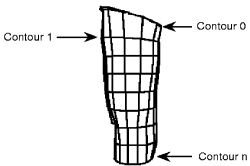
\includegraphics[height=3.5cm]{../images/babski_contours} &
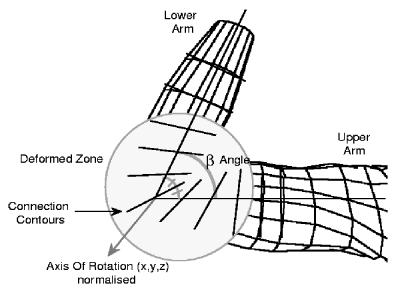
\includegraphics[height=3.5cm]{../images/babski_deformation} \\
{\it(a)} & {\it(b)}
\end{tabular}
\caption[Contoured models for VRML animation]{\label{fig:babskimodels}Contoured models for VRML animation. (a) Model structure for a single body segment. (b) Contour-based deformation around joints. Images taken from \cite{Babski99}.}
\end{center}
\end{figure}
Each segment of the model is defined as a set of contours (see figure \ref{fig:babskimodels}a). The last contour of one segment is also the first contour of the next, ensuring that the body appears seamless. When a joint rotates, the contours near joints are rotated by different amounts, varying from no rotation to half of the rotation of the joint, as shown in figure \ref{fig:babskimodels}b. This contour rotation is applied on both sides of a joint, preserving the model's seamless appearance. The deformation can be executed in real time, due to the efficiency gained by rotating complete contours at once. However, the deformation method suffers from thinning of segments due to the contour rotation, and also cannot handle segments that have more than two joints (e.g. the pelvis).

\section{\label{sec:litreview:conclusion}Conclusion}

In this section we have reviewed the state of the art across all stages of the process of creating models for animation. We have seen that scanning hardware produces accurate surface data, but at far too high a density, and in too unstructured a format to be directly usable. Various modelling techniques have been developed to ease the use of such models, but most require a large amount of manual intervention. A more highly automated method for the creation of these models would be highly desirable, and make the content creation process much easier.

We therefore move on to the description of our layered animation method, which provides an efficient and highly automated method of animating dense scanned surface data.

\chapter{\label{sec:skeletalanim}Control Layer Animation}

In order to create realistic animation of surfaces, we must be able to take realistic animation data and apply it to the surfaces in question. Using skeleton models for animation design is a common practise in computer graphics. The skeleton represents the structure of an articulated figure and is used to define a set of joints and their relationships. It enables an animator to perform simple manipulations of the articulation structure, and obtain complex surface deformations and believable animations.

Some popular methods of performing skeletal animation are described above in section \ref{sec:litreview:animation}, but none of these are ideally suited to our requirements. We require an animation method which can create realistic deformations of a polygon mesh, using efficient methods suited for realtime calculation. The process of preparing the model for animation should also require as little manual intervention as possible. 

We begin our discussion of our layered animation method by defining such a method of skeletal animation, which will allow us to animate a simple control layer mesh using a skeleton structure.

\section{\label{sec:skeletalanim:fitting}Skeleton Fitting}
\begin{figure}
\begin{center}
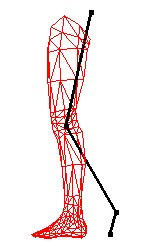
\includegraphics[height=6cm]{../images/fit1}
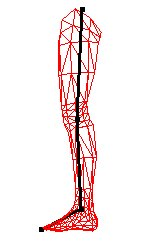
\includegraphics[height=6cm]{../images/fit2}
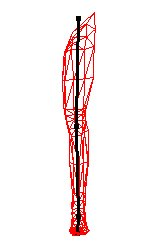
\includegraphics[height=6cm]{../images/fit3}
\caption[Manual Skeleton Fitting]{\label{fig:skeletonfitting} Manual Skeleton Fitting. The skeleton is fitted to the control mesh in two orthogonal views, one joint at a time.}
\end{center}
\end{figure}
The first stage in the process of animating a mesh with a skeleton is to align the two structures correctly, by fitting the skeleton structure to the control mesh. We use a manual interface to individually locate each joint, using two orthogonal viewpoints as shown in figure \ref{fig:skeletonfitting}. This allows the skeleton joint locations to be positioned correctly, ensuring that segment links run through the main structures of the model. The skeleton structure itself is defined manually for each model, but could be constructed interactively with some improvements to the current user interface.

As it is a manual process, the accuracy and repeatability of the skeleton fitting process are limited by the skill of the user. However, in the final system, it is anticipated that this process would be performed by an experienced operator with knowledge of how to position the skeleton model in order to obtain the best results. Incorrectly placed joints will result in unrealistic animation, as joints will appear to rotate around the wrong position.

One possible solution to the repeatability problems would be to generate the skeleton automatically. This would also have the effect of further reducing the manual intervention required in our system. However, no methods for automatic skeleton generation are known of at this time.

\section{\label{sec:skeletalanim:mapping}Control Layer Mapping}

Having located an appropriate skeleton structure inside the mesh we wish to animate, we must now define an automatic mapping between the mesh and the skeleton. Once this mapping is complete, the mesh will be parameterised purely in terms of the skeleton structure, enabling us to drive mesh animation with the skeleton. The mapping must be based purely on the relative locations of skeleton and mesh, as we have no other information available to us, such as higher-level understanding about the two structures. 

We must therefore define a bijective mapping from the space surrounding the skeleton (in which the mesh is embedded) to the skeleton itself. We partition the space into separate regions, each associated with a single segment of the skeleton. Within this region, we then perform a point-to-line mapping to parameterise the mesh vertices in terms of their local segment.

\subsection{\label{sec:skeletalanim:mapping:jointplanes}Joint Planes}
\begin{figure}
\begin{center}
\begin{tabular}{cc}
\setlength{\unitlength}{0.5cm}
\begin{picture}(13,8)
% Joint positions
\put(0,0){\circle*{0.2}}
\put(4,4){\circle*{0.2}}
\put(10,4){\circle*{0.2}}
\put(13,2){\circle*{0.2}}
% Segment links
\put(0,0){\line(1,1){4}}
\put(4,4){\line(1,0){6}}
\put(10,4){\line(3,-2){3}}
% Planes
\put(5,2){\vector(-1,2){2}}
\put(9.33333,2){\vector(1,3){1.3333}}
% Labels
\put(1,0){$\vec{j}_0$}
\put(4.5,4.5){$\vec{j}_1$}
\put(10.5,4.5){$\vec{j}_2$}
\put(13,2.5){$\vec{j}_3$}
\put(3.5,6){$J_1$}
\put(11,6){$J_2$}
\end{picture} &
\setlength{\unitlength}{0.5cm}
\begin{picture}(8,8)
% Joint positions
\put(1,6){\circle*{0.2}}
\put(5,4){\circle*{0.2}}
\put(7,0){\circle*{0.2}}
% Segment links
\thicklines
\put(1,6){\line(2,-1){4}}
\put(5,4){\line(1,-2){2}}
% Joint plane
\thinlines
\put(3,1){\line(0,1){5}}
\put(3,6){\line(2,1){4}}
\put(3,1){\line(2,1){4}}
\put(7,3){\line(0,1){5}}
% Coordinate system
\put(5,4){\vector(0,1){3}}
\put(5,4){\vector(2,1){2}}
\put(5,4){\vector(1,-1){2}}
% Labels
\put(0,6.5){$\vec{j}_{i-1}$}
\put(4,3){$\vec{j}_{i}$}
\put(7.5,0){$\vec{j}_{i+1}$}
\put(7,8){$J_i$}
\put(5.5,6){$\vec{a}_i$}
\put(7.5,5){$\vec{b}_i$}
\put(7.5,2){$\vec{c}_i$}
\end{picture} \\
{\it (a)} & {\it (b)}
\end{tabular}
\caption[Joint Plane Geometry]{\label{fig:jointplanes} Joint Plane Geometry. (a) Joint planes bisect the angles of a skeleton structure. (b) Local coordinate system for a joint plane.}
\end{center}
\end{figure}
We must first partition the space in the region of the skeleton into discrete sections. We do this by defining a {\it joint plane} $J_x\symbol{jointplane}$ for each joint or end effector $\vec{j}_x\symbol{joint}$.

The joint plane $J_x$ is defined as the plane that bisects the joint $\vec{j}_x$, lying equally between the two adjoining segment links, as shown in figure \ref{fig:jointplanes}a. We define $J_x$ using a pair of orthogonal vectors, $\hat{a}_x\symbol{normvector}$ and $\hat{b}_x$. $\hat{a}_x$ is defined as the normal to the plane $P$ defined by the three joint positions $\vec{j}_{x-1}, \vec{j}_x, \vec{j}_{x+1}$, calculated as the normalised cross product of the two adjoining segment vectors.
\begin{eqnarray}
\vec{s}_+ & = & \vec{j}_{x+1} - \vec{j}_x \\
\vec{s}_- & = & \vec{j}_{x-1} - \vec{j}_x \\
\hat{a}_x & = & \frac{\vec{s}_- \times \vec{s}_+}{\|\vec{s}_- \times \vec{s}_+\|}
\end{eqnarray}
$\vec{b}_x$ is defined as the vector that bisects the joint angle, and lies on the plane $P$ as described  above. We calculate this vector as the normalised sum of the two normalised segment vectors:
\begin{eqnarray}
\vec{t} & = & \frac{\vec{s}_-}{\|\vec{s}_-\|} + \frac{\vec{s}_+}{\|\vec{s}_+\|} \nonumber \\
\hat{b}_x & = & \frac{\vec{t}}{\|\vec{t}\|} \label{eqn:jointplaneb}
\end{eqnarray}

Note that $\vec{t}$ is not a new symbol, but simply a temporary vector used to clarify equation \ref{eqn:jointplaneb}. We can also define another useful vector, $\hat{c}_x$, as the cross product of the two vectors $\hat{a}_x$ and $\hat{b}_x$. These three vectors define a local coordinate system, as shown in figure \ref{fig:jointplanes}b.
\begin{equation}
\hat{c}_x = \hat{a}_x \times \hat{b}_x
\end{equation}

\subsubsection{\label{sec:skeletalanim:mapping:jointplanes:special}Special Cases}
There are a number of cases where this formulation is insufficient to define a joint plane. If a joint has multiple child joints, there will be a number of possible values for $\vec{j}_{x+1}$. In this case the average of all these possible values is used for the purposes of plane calculation.

In the case where $\vec{j}_{x-1}$, $\vec{j}_x$ and $\vec{j}_{x+1}$ are colinear, the vector $\vec{a}_x$ is assigned the value of the equivalent vector from the joint plane that lies one level up the skeleton hierarchy, $\vec{a}_{x-1}$. The vector $\vec{b}_x$ is then assigned the value of the normalised cross product $\vec{a}_x \times \vec{s}_-$.

If the joint $\vec{j}_x$ represents an end effector, implying that there is no joint $\vec{j}_{x+1}$ present, $\vec{s}_+$ is assigned the inverted value of $\vec{s}_-$ and the above colinear rule is applied to calculate a valid joint plane.

\subsection{\label{sec:skeletalanim:mapping:pointtoline}Point-To-Line Mapping}

Once we have defined a set of joint planes for a skeleton, we can define a mapping from 3D space onto a single joint segment.  We define the {\it dimensionality} of a segment to be ${\cal S}_n\symbol{segdim}$, where $n$ is one less than the number of bounding planes. We currently only deal with {\it simple} segments, which have only two bounding joint planes, and hence are ${\cal S}_1$. {\it Complex} segments, such as the pelvis, with three or more bounding planes, have a dimensionality of ${\cal S}_n$ where $n>1$, and are discussed below in section \ref{sec:skeletalanim:mapping:complex}.

\begin{figure}
\begin{center}
\setlength{\unitlength}{0.4cm}
\begin{picture}(28,13)
% Points
\put(4,5){\circle*{0.2}}
\put(2,8){\circle*{0.2}}
\put(12,5){\circle*{0.2}}
\put(11,8){\circle*{0.2}}
\put(24,5){\circle*{0.2}}
\put(26,8){\circle*{0.2}}
% Joint planes
\thicklines
\put(1,0){\line(0,1){8}}
\put(1,0){\line(3,1){6}}
\put(7,10){\line(0,-1){8}}
\put(7,10){\line(-3,-1){6}}
\put(21,10){\line(0,-1){8}}
\put(21,10){\line(3,-1){6}}
\put(27,0){\line(0,1){8}}
\put(27,0){\line(-3,1){6}}
% Joint axes
\put(4,5){\vector(0,1){1}}
\put(4,5){\vector(-3,-1){1}}
\put(24,5){\vector(0,1){1}}
\put(24,5){\vector(3,-1){1}}
% Segment links
\put(4,5){\line(1,0){20}}
\thinlines
\put(2,8){\line(1,0){24}}
% Vectors
\put(4,5){\vector(-2,3){2}}
\put(12,5){\vector(-1,3){1}}
\put(24,5){\vector(2,3){2}}
% Labels
\put(6,0){$J_0$}
\put(21,0){$J_1$}
\put(4,4){$\vec{j}_0$}
\put(23,4){$\vec{j}_1$}
\put(1,7){$\vec{p}_0$}
\put(26,7){$\vec{p}_1$}
\put(12,4){$\vec{p}_\alpha$}
\put(11,8.5){$\vec{v}_x$}
\put(6,12.5){$\alpha$}
% Alpha
\put(2,10){\line(0,1){2}}
\put(11,10){\line(0,1){2}}
\put(6,12){\vector(-1,0){4}}
\put(6,12){\vector(1,0){5}}
\end{picture}
\caption[Point To Line Mapping]{\label{fig:pointtoline}Point To Line Mapping}
\end{center}
\end{figure}

The mapping of a 3D point $\vec{v}_x\symbol{vertex}$ onto a line segment is carried out as follows. First of all, $\vec{v}_x$ is projected parallel to the segment, and intersection points $\vec{p}_0\symbol{point}$ and $\vec{p}_1$ calculated with the bounding joint planes, $J_0$ and $J_1$, as shown in figure \ref{fig:pointtoline}.  As the joint planes are infinite in extent, an intersection can always be found, as the planes are never parallel to the projection (segment) vector. 

These intersection points are calculated using standard ray/plane intersection techniques \cite{Lengyel02}. We then calculate a ratio $\alpha_x\symbol{alpha}$, which tells us how far the point $\vec{v}_x$ lies along the segment. The ratio is calculated from the distances between the point $\vec{v}_x$ and the two intersection points.

\begin{equation}
\alpha_x = \frac{\|\vec{v}_x-\vec{p}_0\|}{\|\vec{p}_1-\vec{p}_0\|}
\end{equation}

For instance, a point with $\alpha_x = 0$ would lie on the joint plane $J_0$, while $\alpha_x = 1$ would describe a point lying on the plane $J_1$. A value of 0.5 would define a point lying equidistant between the two planes. The value of $\alpha_x$ describes a plane located between the two bounding joint planes, and which intersects the segment itself at a point $\vec{p}_\alpha$.

\begin{equation} \label{eqn:palpha}
\vec{p}_\alpha = (1 - \alpha_x) \vec{j}_0 + \alpha_x \vec{j}_1
\end{equation}

We then calculate a straight line distance $d_x$ from the point $\vec{p}_\alpha$ to $\vec{v}_x$. 

\begin{equation}
d_x = \|\vec{v}_x - \vec{p}_\alpha\|
\end{equation}

The two parameters $\alpha_x$ and $d_x$ define a circle in 3D space, centred on the point $\vec{p}_\alpha$ and passing through $\vec{v}_x$. In order to uniquely describe the point $\vec{v}_x$, we therefore store a vector $\hat{n}_x$, which is defined as the normal vector to the plane $Q_x$, which passes through $\vec{j}_0$, $\vec{j}_1$ and $\vec{v}_x$. $\vec{p}_0$ and $\vec{p}_1$ also lie on this plane.
\begin{eqnarray}
\vec{t} & = & (\vec{j}_1 - \vec{j}_0) \times (\vec{v}_x - \vec{j}_0) \nonumber \\
\hat{n}_x & = & \frac{\vec{t}}{\|\vec{t}\|}
\end{eqnarray}
Note again that $\vec{t}$ is not a new symbol, but a temporary vector used for clarification. The normal vector $\hat{n}_x$ describes the rotation of the point $\vec{v}_x$ around the segment, and along with the two parameters $\alpha_x$ and $d_x$, uniquely describes the position of the point $\vec{v}_x$. Upon animation, these parameters allow us to deform the 3D position of $\vec{v}_x$ as described below in section \ref{sec:skeletalanim:anim:control}.

\subsection{\label{sec:skeletalanim:mapping:complex}Complex Segments}

The method described above defines a mapping from 3D space onto a line segment. However, complex segments are not represented by a line segment, but by a simplex, the dimensionality of which depends on that of the segment. For instance, an ${\cal S}_2$ segment with three bounding joints would be represented by a triangle, while an ${\cal S}_3$ segment with four bounding joints would be represented by a tetrahedron. The line segment is, of course, the one-dimensional simplex, as is appropriate for an ${\cal S}_1$ segment with two bounding planes. Complex segments are common in skeletal structures; for instance, the human body, while containing mostly ${\cal S}_1$ segments, contains two ${\cal S}_3$ segments at the pelvis and shoulders, and no less than four ${\cal S}_5$ segments, in the hands and feet.

We must therefore generalise our mapping method to map a volume to an $n$-dimensional simplex. The mapping solution defined above works well for ${\cal S}_1$ segments. Additionally, normal-volume mapping, a similar method for mapping points to surfaces described later in section \ref{sec:scandata:pointtosurface}, could be adapted for ${\cal S}_2$ segments. This suggests that it should be possible to formulate a general method of mapping points to ${\cal S}_n$ segments. However, this has not been successful to date, and it is likely that a general mapping solution would be polynomial with degree $n$ or even greater, making the mapping excessively complex even for commonly-occurring segments such as ${\cal S}_5$.

Therefore, we deal only with ${\cal S}_1$ segments from now on, and fix points that lie within complex segments rigidly to that segment, without performing any mapping or deformation.

\subsection{\label{sec:skeletalanim:mapping:mesh}Mesh Mapping}

We define a triangle mesh as a combination of two sets, ${\cal V}\symbol{verts}$ and ${\cal T}\symbol{tris}$. ${\cal V}$ represents the set of vertices in the mesh, and ${\cal T}$ represents the set of triangles, which form the mesh topology.

In order to map a complete mesh to a skeleton, we map each mesh vertex individually. However, we must decide which segment each vertex will map to. In order to calculate this, we must decide which pair of joint planes the vertex lies between. We map each control mesh vertex $\vec{v}_x \in {\cal V}$ to each segment in turn, and calculate its $\alpha_x$ value for that segment. The vertex is assigned to the segment for which the value of $\alpha_x$ lies between 0 and 1, i.e. the vertex $\vec{v}_x$ lies between the joint planes. If this is the case for more than one segment, we calculate the value of $d_x$ for each segment, and assign the vertex to the segment for which it has the lowest value of $d_x$.

\section{\label{sec:skeletalanim:anim}Animation}

Once we have mapped a mesh to the skeleton structure, we can animate that skeleton structure in order to animate the surface of the mesh. This process involves rebuilding the mesh structure from the parameterised representation we have calculated, based on the animated positions of the skeleton's joints.

\subsection{\label{sec:skeletalanim:anim:skeleton}Skeleton Motion}

The animation of the skeleton can be driven by a number of different data sources, from manual keyframed animation, to motion capture systems. In each case however, the data itself is the same. Each frame of animation consists of a set of joint angles which are applied to the joints of the skeleton. The skeleton is then traversed, starting from the root joint and proceeding down the hierarchy, and the cumulative rotation is applied to the default joint positions to position the skeleton into the correct pose. Alternative methods could deliver updated joint positions directly to the skeleton without the use of rotations, but these have the disadvantage that segment lengths are not necessarily preserved, which adversely affects the realism of the animation.

\subsection{\label{sec:skeletalanim:anim:control}Control Layer Deformation}

As the skeleton layer is animated, the joints of the skeleton will change position, which will have the effect of changing the joint planes. As we have parameterised the space around a segment in terms of the joint planes, movement of those planes will deform the parameterised space, and hence the mesh embedded within it. For each animation frame, we need to recalculate a deformed vertex position $\vec{v}_x'$ for each original vertex $\vec{v}_x$. Firstly, the joint planes are updated, by rotating each joint plane by half of the rotation of its associated joint. This ensures that the joint plane still bisects the joint angle.

For each vertex $\vec{v}_x \in {\cal V}$, we can calculate a deformed vertex position $\vec{v}_x'$ using the stored parameters $\alpha_x$, $d_x$, and $\hat{n}_x$. We start by calculating a pair of vectors $\hat{s}_0$ and $\hat{s}_1$ on the bounding planes. These vectors define the direction in which the deformed points $\vec{p}_0$ and $\vec{p}_1$ lie on the rotated joint planes.
\begin{eqnarray} \label{eqn:normals}
\hat{s}_0 & = & \hat{c}_0 \times \hat{n}_x \\ 
\hat{s}_1 & = & \hat{c}_1 \times \hat{n}_x
\end{eqnarray}
We then calculate a vector $\vec{s}_\alpha$ as a linear interpolation of $\hat{s}_0$ and $\hat{s}_1$, as well as a point $\vec{p}_\alpha$ on the line segment. This tells us the point on the segment that the original $\vec{v}_x$ mapped to, and the direction in which the deformed $\vec{v}_x'$ should lie.
\begin{eqnarray}
\vec{s}_\alpha & = & (1 - \alpha_x) \hat{s}_0 + \alpha_x \hat{s}_1 \\
\vec{p}_\alpha & = & (1 - \alpha_x) \vec{j}_0' + \alpha_x \vec{j}_1' 
\end{eqnarray}
We then calculate the new vertex position $\vec{v}_x'$ by multiplying the $\vec{s}_\alpha$ by the stored distance value $d_x$, and adding to $\vec{p}_\alpha$.
\begin{equation}
\vec{v}_x' = \vec{p}_\alpha + d_x \vec{s}_\alpha
\end{equation}
\begin{figure}
\begin{center}
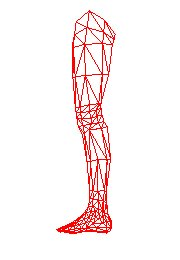
\includegraphics[width=3.18cm]{../images/low_leg_1}
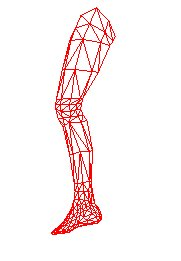
\includegraphics[width=3.18cm]{../images/low_leg_2}
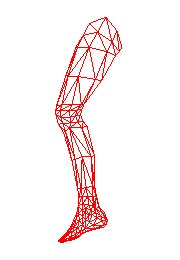
\includegraphics[width=3.18cm]{../images/low_leg_3}
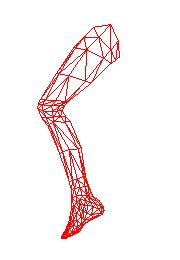
\includegraphics[width=3.18cm]{../images/low_leg_4}
\caption[Control Mesh Animation]{\label{fig:controlmesh} Control Mesh Animation.}
\end{center}
\end{figure}
This formulation gives an efficient deformation for each point, well suited for realtime calculation. Figure \ref{fig:controlmesh} illustrates the skeletal animation of a simple mesh, showing how the shape of the mesh deforms as the skeleton bends.

\subsection{\label{sec:skeletalanim:anim:collapse}Segment Collapse}

The above method works well for small changes in the pose of the skeleton, but large angles at joints can introduce errors. The linear interpolation of the plane vectors introduces thinning effects near joints, orthogonal to the axis of the joint rotation. Also caused by this is the complete collapse of segments under twisting rotations. Both of these effects are highly undesirable.

A method of avoiding these problems was described by Wei Sun in \cite{Sun01}. This method compensates for the thinning effects by introducing a term into the reconstruction equations that causes a reconstructed point to maintain a fixed distance from the nearest point on the segment, or from a joint centre if that is closer. This method prevents the thinning of the surface, as well as sharp creases near joints, giving a smooth deformation of the mesh surface.

\section{\label{sec:skeletalanim:vrml}VRML Implementation}
\nomenclature{\bf VRML}{The Virtual Reality Modelling Language, a programming language for describing 3D scenes and objects.}
In order to demonstrate the efficiency of the skeletal animation method described above, we have created an implementation of the algorithm in the VRML97 3D modelling language \cite{VRML97}. In order to do this, we also describe a novel method for the animation of deformable models in VRML, which we originally introduced in \cite{Smith00}.

\subsection{\label{sec:skeletalanim:vrml:hanim}H-Anim Compliant Humans}

We base our method on the existing H-Anim 1.1 specification \cite{HANIM99} for the animation of articulated characters in VRML. The H-Anim standard defines a set of VRML extensions which are used to represent articulated models, in particular humanoid figures. These extensions are implemented using the PROTO mechanism, which allows new VRML nodes to be defined in terms of the standard set of nodes \footnote{In the following description, names of VRML nodes are written in {\bf bold} type, while field and other names are written in {\it italics}.}

H-Anim defines a number of new VRML nodes; firstly, it defines the {\bf Humanoid} node, which acts as a container for an articulated model structure. This node contains within it a hierarchy of {\bf Joint} nodes, which form the skeleton structure itself. The skeleton is posed by assigning rotation values to each of these joint nodes. Each {\bf Joint} has a name associated with it, assigned by a special naming scheme. For instance, the left shoulder joint is named {\it l\_shoulder}. A single joint forms the root of the hierarchy, named {\it HumanoidRoot}. 

The joints define the articulation structure of the model, but the geometry of the body is defined inside {\bf Segment} nodes. Each {\bf Joint} contains a single {\bf Segment}, corresponding to the part of the body directly affected by that joint and named accordingly. For instance, the {\it l\_shoulder} joint will have a child segment named {\it l\_upperarm}. {\bf Segment}s contain geometry information for that section of the model, so the {\it l\_upperarm} will typically contain an {\bf IndexedFaceSet} node containing a rigid 3D model for the upper arm.

A {\bf Segment} node can also contain any number of {\bf Site} nodes. These nodes store single 3D points, for use as end effectors, or attachment points for clothing and accessories. If we consider a segment representing the left hand, {\it l\_hand}, it will contain a site representing an end effector, named {\it l\_hand\_tip}.

\subsection{\label{sec:skeletalanim:vrml:extentions}Extending H-Anim for Seamless Models}
As VRML97 does not allow non-rigid transformations of objects, it is impossible to represent deformable seamless\footnote{A seamless surface will be C0 continuous, i.e. will not contain any cracks.} models using pure VRML. However, the VRML97 {\bf Script} node allows a programmer to add functionality to the language by using Java \cite{Gosling00} or ECMAScript \cite{ECMA99} to write code that can be executed as part of a VRML scene. We can implement the mesh deformation algorithm using this facility, but we must first define a VRML structure which will represent the seamless model. We base our structure around H-Anim 1.1, but add a number of new elements. We take a different approach to previous methods \cite{Babski99}, and define the surface as a single polygon mesh, while separating geometric and topological properties.

First, we calculate which segment each vertex should be assigned to, using the method described in section \ref{sec:skeletalanim:mapping:mesh}. The vertices are then re-ordered so that they are arranged in contiguous sets of vertices that are assigned to the same segment. The set of vertices for each segment is then stored in the {\it coord} field of the appropriate {\bf Segment} node.

We then define a new node, {\bf MeshBody}  (see figure \ref{fig:meshbodyproto}), to store the remaining mesh data including topology, texture and colour information. This node is implemented as a combination of an {\bf IndexedFaceSet} and a {\bf Script} node. The mesh data is stored in the {\bf IndexedFaceSet} part, and the {\bf Script} contains a Java or ECMAScript implementation of the deformation engine. The {\bf MeshBody} node itself is stored inside a new field which we add to the {\bf Humanoid} node, called {\it meshBody}. The extended {\bf Humanoid} node is shown in figure \ref{fig:humanoidproto}.

\begin{figure}
\renewcommand{\baselinestretch}{1}
\scriptsize
\begin{verbatim}
PROTO MeshBody [
 exposedField SFString   name             ""
 exposedField MFString   info             []
 exposedField SFNode     appearance       NULL
 exposedField SFNode     color            NULL
 exposedField SFNode     normal           NULL
 exposedField SFNode     texCoord         NULL     
 field        SFBool     ccw              TRUE
 field        MFInt32    colorIndex       []
 field        SFBool     colorPerVertex	  TRUE
 field        SFBool     convex           TRUE
 field        MFInt32    coordIndex       []
 field        SFFloat    creaseAngle      0
 field        MFInt32    normalIndex      []
 field        SFBool     normalPerVertex  TRUE
 field        SFBool     solid            TRUE
 field        MFInt32    texCoordIndex    []
 field        SFBool     mustEvaluate     FALSE
 field        SFNode     humanoid         NULL
 field        MFString   url              []
 eventIn      SFTime     update
]
{
  Group {
    children [
      Shape {
        appearance IS appearance
        geometry IndexedFaceSet {
          color IS color
          normal IS normal
          texCoord IS texCoord
          ccw IS ccw
          colorIndex IS colorIndex
          colorPerVertex IS colorPerVertex
          convex IS convex
          coordIndex IS coordIndex
          coord DEF BODYCOORDS Coordinate {}
          creaseAngle IS creaseAngle
          normalIndex IS normalIndex
          normalPerVertex IS normalPerVertex
          solid IS solid
          texCoordIndex IS texCoordIndex
        }
      }
      DEF SEAMLESSBODY Script {
        url IS url
        directOutput TRUE
        mustEvaluate IS mustEvaluate
        field SFNode humanoid IS humanoid
        field SFNode bodyCoords USE BODYCOORDS
        eventIn SFTime update IS update
      }
    ]
  }
}
\end{verbatim}
\caption[The MeshBody Prototype]{\label{fig:meshbodyproto} The {\bf MeshBody} Prototype. The new node is basically a fusion of an {\bf IndexedFaceSet} and a {\bf Script}.}
\end{figure}

\begin{figure}[t]
\renewcommand{\baselinestretch}{1}
\scriptsize
\begin{verbatim}
PROTO Humanoid [
 exposedField SFVec3f    center           0 0 0
 exposedField MFNode     humanoidBody     [ ]
 exposedField MFString   info             [ ]
 exposedField MFNode     joints           [ ]
 exposedField SFNode     meshBody         NULL              # NEW
 exposedField SFString   name             ""
 exposedField SFRotation rotation         0 0 1 0
 exposedField SFVec3f    scale            1 1 1
 exposedField SFRotation scaleOrientation 0 0 1 0
 exposedField MFNode     segments         [ ]
 exposedField MFNode     sites            [ ]
 exposedField SFVec3f    translation      0 0 0
 exposedField SFString   version          "1.1"
 exposedField MFNode     viewpoints       [ ]
]
{
  Transform {
    center IS center
    rotation IS rotation
    scale IS scale
    scaleOrientation IS scaleOrientation
    translation IS translation
    children [
      Group {
        children IS viewpoints
      }
      Group {
        children IS humanoidBody
      }
      Group {                                               # NEW
        children IS meshBody                                # NEW
      }                                                     # NEW
    ]
  }
}
\end{verbatim}
\caption[The Extended Humanoid Prototype.]{\label{fig:humanoidproto} The Extended {\bf Humanoid} Prototype. Our extensions are marked with comments.}
\end{figure}

\subsection{\label{sec:skeletalanim:vrml:animation}Animation}
During a single frame of animation, a set of rotations are applied to the joints in the structure, posing the skeleton. The Java code inside the {\bf Script} node then traverses the hierarchy, deforming the vertices contained in the {\it coord} field of each {\bf Segment} appropriately, and merging them into a single vertex list which is placed into the {\bf IndexedFaceSet} section of the {\bf MeshBody} node, in order to set the geometry of the mesh for display. This method deforms the mesh seamlessly by modifying the vertices of a single mesh separately.

\subsection{\label{sec:skeletalanim:vrml:engine}The Deformation Engine}

The actual deformation process is performed wholly within a Java program stored in the {\bf Script} section of the {\bf MeshBody} node. The internal structure of the script consists of an {\it init} function, which is called when the model is loaded, and an {\it eventsProcessed} function which is called once per frame.

The {\it init} method traverses the skeleton hierarchy, calculating joint planes and performing the mapping process described in section \ref{sec:skeletalanim:mapping}. The joint planes and mapped vertices are cached inside the script for later reconstruction. 

\begin{figure}
\begin{center}
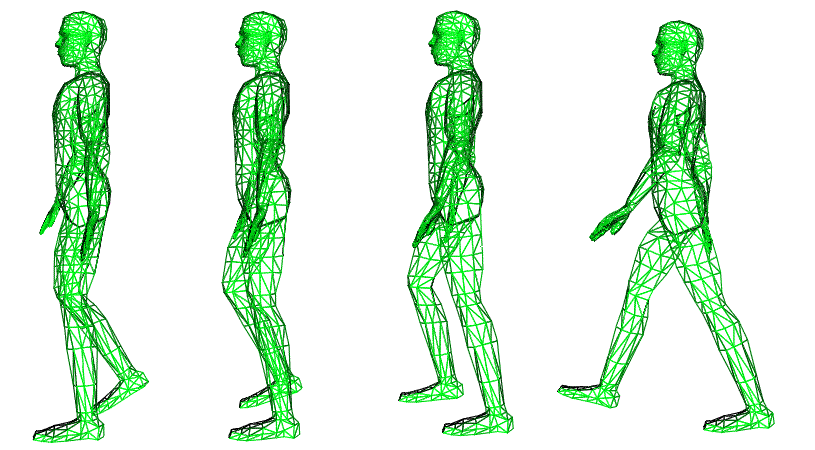
\includegraphics[width=14cm]{../images/simpleanimation}
\caption[Seamless VRML Humans]{\label{fig:simplesegments} Seamless VRML Humans. This figure shows our skeletal animation technique, applied to a human body model in VRML. }
\end{center}
\end{figure}

The {\it eventsProcessed} method is then called before each frame is displayed on screen. This method traverses the skeleton hierarchy again, reading the joint rotations and updating its internal cache of joint planes. The reconstruction process described in section \ref{sec:skeletalanim:anim} is then carried out for each vertex. The vertices are fused into a single list, and output into the {\it bodyCoords} field of the {\bf Script}, which is in turn a reference to the {\it coord} field of the {\bf IndexedFaceSet}. The VRML browser then displays the deformed mesh, an example of which is shown in figure \ref{fig:simplesegments}.

The VRML structures only define the interface to the deformation engine script, not its behaviour. Therefore,  any deformation scheme could be used in conjunction with this structure, not necessarily the one we describe above. The deformation engine must simply read rotations from the hierarchy, read coordinates from the segments, and output a  set of deformed coordinates into its {\it bodyCoords} field each frame. The deformation engine can be treated as a `black box' system.

\subsection{\label{sec:skeletalanim:vrml:hanim2001}H-Anim 2001}

Since this method was introduced, elements of the design have been integrated into the H-Anim 2001 specification \cite{HANIM2001}. This latest version of the specification adds support for seamless deformable models, using a technique based in part on that presented above. The {\bf Humanoid} stores a single list of coordinates, which are referenced by a set of {\bf IndexedFaceSet} nodes which form the surface of the seamless object. Each {\bf Segment} then contains a list of indices of coordinates that are affected by that segment, as well as a set of weights for those vertices. The {\bf Humanoid} node also contains a script, which implements a deformation engine. The specification is designed to include a generic vertex blending deformation engine, but there is no reason why a different animation algorithm could not be used instead.

\section{\label{sec:skeletalanim:results}Results}

\begin{figure}
\begin{center}
\begin{tabular}{ccc}
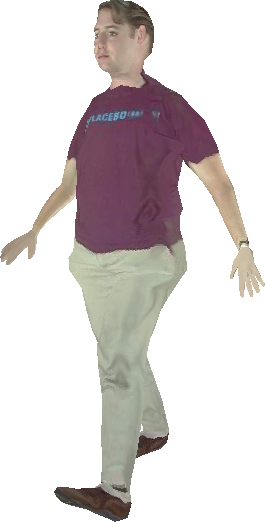
\includegraphics[height=5cm]{../images/james_texture1} &
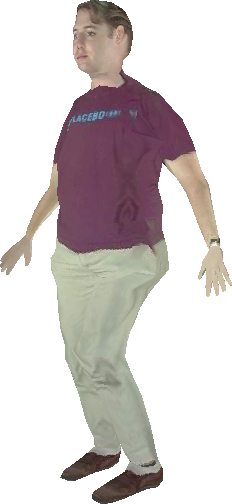
\includegraphics[height=5cm]{../images/james_texture2} &
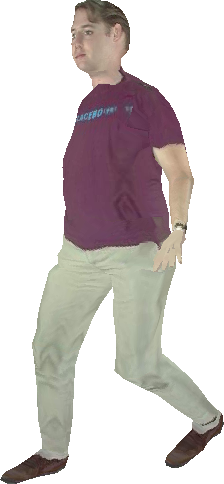
\includegraphics[height=5cm]{../images/james_texture3} \\
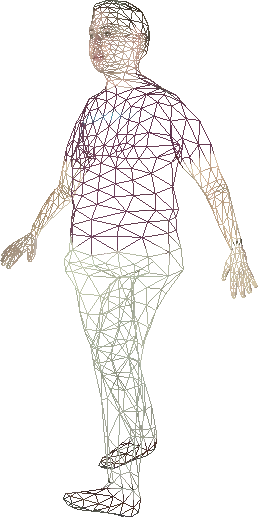
\includegraphics[height=5cm]{../images/james_wire1} &
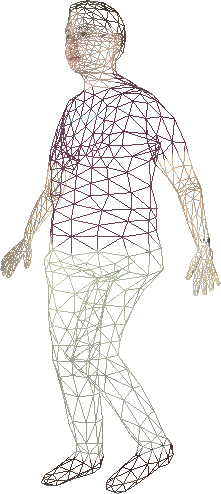
\includegraphics[height=5cm]{../images/james_wire2} &
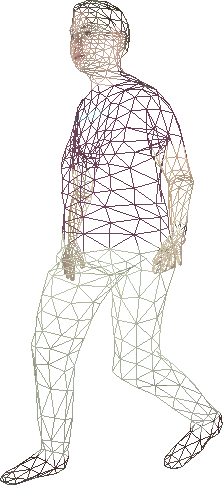
\includegraphics[height=5cm]{../images/james_wire3} \\
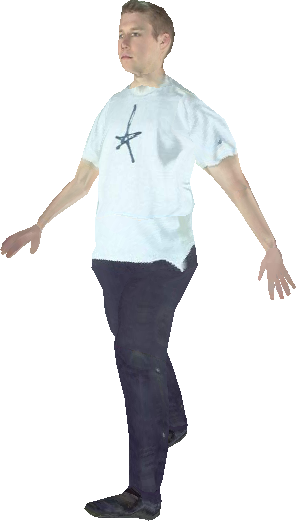
\includegraphics[height=5cm]{../images/warren_texture1} &
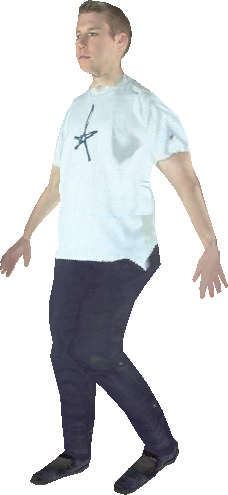
\includegraphics[height=5cm]{../images/warren_texture2} &
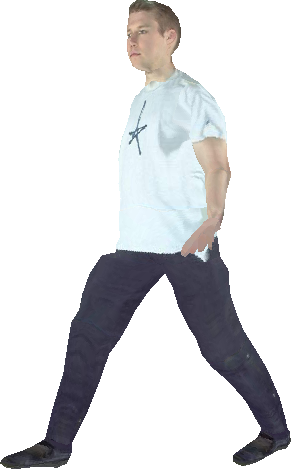
\includegraphics[height=5cm]{../images/warren_texture3} \\
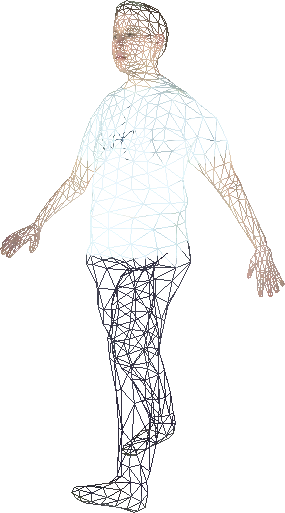
\includegraphics[height=5cm]{../images/warren_wire1} &
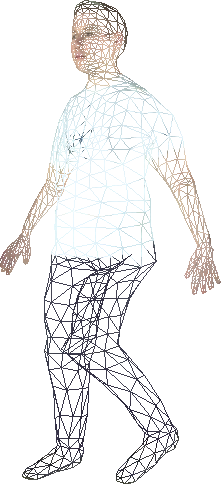
\includegraphics[height=5cm]{../images/warren_wire2} &
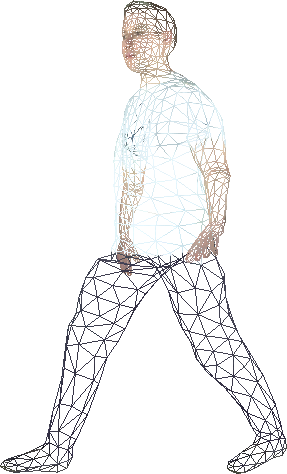
\includegraphics[height=5cm]{../images/warren_wire3} \\
\end{tabular}
\caption[Control Mesh Animation]{\label{fig:controlanim} Control Mesh Animation, showing animation of two human models in VRML, using our deformation technique. The models were generated using the AvatarBooth body scanner from \citet{AvatarMe}.}
\end{center}
\end{figure}

Figure \ref{fig:controlanim} shows our skeletal animation technique applied to a pair of human body models. These models were animated in real time using the VRML implementation of our deformation engine. Surface discontinuities can be seen in places, as the implementation only deals with ${\cal S}_1$ segments, as discussed earlier. Complex segments such as the pelvis are transformed rigidly with their parent joint.

\section{\label{sec:skeletalanim:conclusion}Conclusion}

We have presented a novel method of performing skeletal animation, which uses a fully-automatic mapping process to perform deformations of the surface based on a manually positioned skeleton structure. The algorithm is efficient, able to execute in real time even when run inside an interpreted VRML script. However, the algorithm cannot currently support deformation of complex body segments, as no method has yet been developed to extend the automatic mapping process to higher dimensions.

We have also presented a novel method of defining seamless deformable objects in VRML97, which has since been integrated in part into the H-Anim 2001 specification, which is intended for ISO standardisation.

Our skeletal animation method allows an animator to animate a low-resolution mesh in real time, by manipulating the skeleton structure. The next stage in our layered animation method is to apply the animation of this low resolution mesh to the dense scanned data that we actually wish to deform. This should enable accurate translation of the low resolution animation to a highly detailed surface.

\subsection{\label{sec:skeletalanim:conclusion:future}Future Work}

The skeletal animation method presented in this chapter can be improved in a number of ways. Firstly, as discussed in section \ref{sec:skeletalanim:mapping:complex}, we can currently only cope with simple segments with two bounding joints. This is insufficient to animate complex models effectively, and so the method should be extended to support animation of complex segments. Additionally, it may be useful to use a higher order function to interpolate along each segment, rather than a simple linear interpolation. This has not been investigated however, and would need further research, but has the potential to create mathematically smooth animation of the surface.

During development of the linear interpolation method described above, another method was proposed which has not been implemented, but which is worthy of further research. Instead of using a linear interpolation of end plane points, we propose a method of performing skeletal animation using quaternion-based interpolation. The $\alpha_x$ coordinate of a point would still be calculated as above, but instead of calculating $d_x$ and $\hat{n}_x$, we simply store $\vec{q}_x$, which is a vector from the point $\vec{p}_\alpha$ to $\vec{v}_x$. Each frame, a rotation is calculated that rotates $J_0$ onto $J_1$, and this rotation is interpolated along the segment using spherical linear interpolation of quaternions \cite{Lengyel02}. The interpolated rotation is applied to each vector $\vec{q}_x$ to create a deformed version of each point. This method should reduce collapse due to twisting, giving a more robust animation of the control layer. 

\chapter{\label{sec:scandata} Animation of Scanned Data}

In chapter \ref{sec:skeletalanim}, we presented a method of animating a polygon mesh using skeletal motion to drive changes in the geometry of a simple mesh. However, we are ultimately interested in animating extremely dense meshes, rather than the low-detail meshes discussed above. It would be possible to apply the above method directly to such dense data, but such a solution would not satisfy our requirement of interactive control of the animation, as animating a dense mesh directly would require a prohibitive amount of computation. Therefore, we continue with the layered animation approach introduced in chapter \ref{sec:introduction} and use the dense scan data to build a top-level {\it detail layer}.

We require a number of properties for our detail layer surface; firstly, it must be defined in terms of the control layer so that it can be animated by deformations of that layer. Secondly, these animations should be smooth and seamless; they should not introduce cracks or discontinuities that were not present in the original data.

In order to redefine the detail layer in terms of the control layer, we need to define a mapping from a volume to a 2D surface, as the control layer is a 2D surface embedded in ${\mathbb R}^3$. The mapping should be continuous across the space, with no sharp boundaries. It should also be capable of smooth animation, so that the space deforms smoothly as the control layer moves. We also require this mapping to be invertible, as we wish to both perform a mapping of the detail layer to the control layer, and also the inverse, i.e. reconstruction of the detail layer surface. The mapping function must therefore be bijective in our region of interest.

We perform this mapping using a {\it normal volume} approach, which is similar to the skeletal mapping method described above, in that it defines a point in space in terms of a point on a known surface, plus an offset along a normal vector. This formulation allows us to represent a detailed mesh in terms of a simpler one, and to smoothly animate the two meshes together.

\section{\label{sec:scandata:normalvolume}The Normal Volume}
\nomenclature{\bf Normal Volume}{A volumetric envelope which extends above and below a triangle surface, whose boundaries are defined by the normals at the triangle vertices.}
\begin{figure}
\begin{center}
\setlength{\unitlength}{0.4cm}
\begin{picture}(21,11)
% M
\thicklines
\put(2,4){\circle*{0.2}}
\put(2,4){\line(4,3){4}}
\put(6,7){\circle*{0.2}}
\put(6,7){\line(4,-1){4}}
\put(10,6){\circle*{0.2}}
\put(10,6){\line(1,0){4}}
\put(14,6){\circle*{0.2}}
\put(14,6){\line(2,-1){4}}
\put(18,4){\circle*{0.2}}
% M+
\put(1,8){\line(4,3){4}}
\put(5,11){\line(6,-1){6}}
\put(11,10){\line(1,0){4}}
\put(15,10){\line(5,-2){5}}
% M-
\put(3,0){\line(4,3){4}}
\put(7,3){\line(2,-1){2}}
\put(9,2){\line(1,0){4}}
\put(13,2){\line(3,-2){3}}
% Normals
\thinlines
\put(3,0){\vector(-1,4){2}}
\put(7,3){\vector(-1,4){2}}
\put(9,2){\vector(1,4){2}}
\put(13,2){\vector(1,4){2}}
\put(16,0){\vector(1,2){4}}
% Labels
\put(2,0){$\vec{v}_x^-$}
\put(1,4){$\vec{v}_x$}
\put(0,8){$\vec{v}_x^+$}
\put(1.5,6.5){$\vec{n}_x$}
\put(17,0){$M^-$}
\put(19,4){$M$}
\put(21,8){$M^+$}
\end{picture}
\caption[Offset Surfaces]{\label{fig:offsetsurface} Offset surface of a mesh. The two offset surfaces $M^+$ and $M^-$ define a volumetric envelope around $M$.}
\end{center}
\end{figure}

In order to perform this mapping, we use the concept of the normal volume or {\it fundamental prism}, introduced by \citet{Cohen96} and which was extended by Adrian Hilton in \cite{Sun01}. We first create a volumetric envelope, which is defined over the mesh $M$ that we want to map to, and which completely encloses it. This envelope is formed by taking each vertex $\vec{v}_x \in {\cal V}_M$ and translating it along its normal vector $\vec{n}_x$ by two distances $d^+$ and $d^-$, creating two new points, ${\vec{v}_x}^+$ and ${\vec{v}_x}^-$, as shown in figure \ref{fig:offsetsurface}. This defines two offset surfaces, $M^+$ and $M^-$.
\begin{eqnarray}
\vec{v}_x^+ & = & \vec{v}_x + d^+\vec{n}_x \\
\vec{v}_x^- & = & \vec{v}_x + d^-\vec{n}_x
\end{eqnarray}

\begin{figure}
\begin{center}
\setlength{\unitlength}{0.5cm}
\begin{tabular}{cc}
\begin{picture}(13,14)
% triangles
\thicklines
\put(5,1){\line(2,1){2}}
\put(5,1){\line(3,-1){3}}
\put(7,2){\line(1,-2){1}}
\put(3,6){\line(2,1){4}}
\put(3,6){\line(3,-1){6}}
\put(7,8){\line(1,-2){2}}
\put(1,11){\line(2,1){6}}
\put(1,11){\line(3,-1){9}}
\put(7,14){\line(1,-2){3}}
% points
\put(5,1){\circle*{0.2}}
\put(7,2){\circle*{0.2}}
\put(8,0){\circle*{0.2}}
\put(3,6){\circle*{0.2}}
\put(7,8){\circle*{0.2}}
\put(9,4){\circle*{0.2}}
\put(1,11){\circle*{0.2}}
\put(7,14){\circle*{0.2}}
\put(10,8){\circle*{0.2}}
% normals
\thinlines
\put(5,1){\line(-2,5){4}}
\put(7,2){\line(0,1){12}}
\put(8,0){\line(1,4){2}}
% vertex labels
\put(4,0.5){$\vec{v}_a^-$}
%\put(7.5,2){$\vec{v}_b^-$}
%\put(8.5,0){$\vec{v}_c^-$}
\put(2,5.5){$\vec{v}_a$}
%\put(7.5,7){$\vec{v}_b$}
%\put(9.5,3){$\vec{v}_c$}
\put(0,10.5){$\vec{v}_a^+$}
%\put(7.5,12){$\vec{v}_b^+$}
%\put(10.5,6){$\vec{v}_c^+$}
% normal labels
\put(2.5,8){$\hat{n}_a$}
%\put(6,9){$\vec{n}_b$}
%\put(8.8,5){$\vec{n}_c$}
% triangle labels
\put(11,1){$t_x^-$}
\put(11,5){$t_x$}
\put(11,11){$t_x^+$}
\end{picture} &
\begin{picture}(13,14)
% triangles
\thicklines
\put(5,1){\line(2,1){2}}
\put(5,1){\line(3,-1){3}}
\put(7,2){\line(1,-2){1}}
\put(7,2){\line(2,-1){2}}
\put(8,0){\line(1,1){1}}
\put(3,6){\line(2,1){4}}
\put(3,6){\line(3,-1){6}}
\put(7,8){\line(1,-2){2}}
\put(7,8){\line(2,-1){4}}
\put(9,4){\line(1,1){2}}
\put(1,11){\line(2,1){6}}
\put(1,11){\line(3,-1){9}}
\put(7,14){\line(1,-2){3}}
\put(7,14){\line(2,-1){6}}
\put(10,8){\line(1,1){3}}
% points
\put(5,1){\circle*{0.2}}
\put(7,2){\circle*{0.2}}
\put(8,0){\circle*{0.2}}
\put(9,1){\circle*{0.2}}
\put(3,6){\circle*{0.2}}
\put(7,8){\circle*{0.2}}
\put(9,4){\circle*{0.2}}
\put(11,6){\circle*{0.2}}
\put(1,11){\circle*{0.2}}
\put(7,14){\circle*{0.2}}
\put(10,8){\circle*{0.2}}
\put(13,11){\circle*{0.2}}
% normals
\thinlines
\put(5,1){\line(-2,5){4}}
\put(7,2){\line(0,1){12}}
\put(8,0){\line(1,4){2}}
\put(9,1){\line(2,5){4}}
\end{picture} \\
{\it (a)} & {\it (b)}
\end{tabular}
\caption[The Normal Volume]{\label{fig:normalvolume} The Normal Volume. (a) The normal volume of a single triangle $t_x$. (b) Adjacent normal volumes form a continuous envelope.}
\end{center}
\end{figure}

As a triangle is made up of a triplet of mesh vertices $t_x\symbol{triangle} = [\vec{v}_a,\vec{v}_b,\vec{v}_c]$, each triangle $t_x \in {\cal T}$ will therefore have a corresponding pair of offset triangles, ${t_x}^+$ and ${t_x}^-$, as illustrated in figure \ref{fig:normalvolume}a. The volume contained within this prism is called the normal volume of the triangle $t_x$, $N_x$\symbol{nv}. The normal volume can also be defined as the union of all offset polygons $t_x^d$ at distance $d$, for $d^- \leq d \leq d^+$.
\begin{eqnarray}
t_x^d & = & [\vec{v}_a^d,\vec{v}_b^d,\vec{v}_c^d] \\
N_x & = & \bigcup^{d^+}_{d=d^-} t_x^d
\end{eqnarray}
The union of all normal volumes ${\cal N}$\symbol{nvset} (see equation \ref{eqn:nvset}) defines a volumetric envelope which encloses the original mesh $M$, and each point $p$ within this envelope lies within a particular normal volume $N_x$, which has a related triangle $t_x$. Therefore, as long as the detail layer mesh ${\cal T_D}$ of our model is wholly contained within the volumetric envelope of the control layer ${\cal N_C}$, each vertex in the detail layer mesh $\vec{v}_x \in {\cal V_D}$ can be associated with a control layer triangle $t_x$.

\begin{equation} \label{eqn:nvset}
{\cal N} = \bigcup^{n-1}_{x=0} N_x
\end{equation}

\subsection{\label{sec:scandata:normalvolume:interpolation}Normal Interpolation}

\begin{figure}
\begin{center}
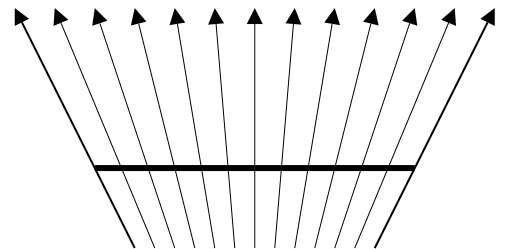
\includegraphics[width=7cm]{../images/normals}
\caption[Normal Interpolation]{\label{fig:normalinterpolation} Normal Interpolation. A slice through a normal volume, showing how triangle normals are interpolated across the surface of the associated triangle.}
\end{center}
\end{figure}

A planar polygon in 3D space has a single normal vector, which is perpendicular to the polygon surface. In a polygon mesh, however, each vertex also has a normal vector, defined as a combination of the surrounding face normals. In our normal volume representation, however, a single triangle does not have a single normal. Each point on the triangle surface will have a unique normal value, as shown in figure \ref{fig:normalinterpolation}. 

The normals are linearly interpolated across the surface of the triangle, and the normal $\vec{n}_j$ at any point $p_j$ on the triangle surface can be expressed as a linear combination of the three vertex normals:

\begin{equation} \label{eqn:interpolatednormals}
\vec{n}_j = \omega_a\hat{n}_a + \omega_b\hat{n}_b + \omega_c\hat{n}_c
\end{equation}

Where $\hat{n}_x\symbol{normal}$ is the surface normal at the vertex $\vec{v}_x$, and $\omega_x$ is an areal coordinate component for that point and vertex, as described below in section \ref{sec:scandata:pointtosurface:areal}. This kind of normal interpolation technique is often used in Phong shading of polygon meshes \cite{Phong75}. 

\subsection{\label{sec:scandata:normalvolume:collapse}Normal Volume Collapse}

\begin{figure}
\begin{center}
\setlength{\unitlength}{0.5cm}
\begin{picture}(9,12)
% triangles
\thicklines
\put(8,1){\line(-2,-1){2}}
\put(8,1){\line(-3,1){3}}
\put(6,0){\line(-1,2){1}}
\put(4,5){\line(2,1){2}}
\put(4,5){\line(3,-1){3}}
\put(6,6){\line(1,-2){1}}
\put(0,9){\line(2,1){6}}
\put(0,9){\line(3,-1){9}}
\put(6,12){\line(1,-2){3}}
% points
\put(8,1){\circle*{0.2}}
\put(6,0){\circle*{0.2}}
\put(5,2){\circle*{0.2}}
\put(4,5){\circle*{0.2}}
\put(6,6){\circle*{0.2}}
\put(7,4){\circle*{0.2}}
\put(0,9){\circle*{0.2}}
\put(6,12){\circle*{0.2}}
\put(9,6){\circle*{0.2}}
% normals
\thinlines
\put(4,5){\line(1,-1){4}}
\put(4,5){\vector(-1,1){4}}
\put(6,6){\line(0,-1){6}}
\put(6,6){\vector(0,1){6}}
\put(7,4){\line(-1,-1){2}}
\put(7,4){\vector(1,1){2}}
% triangle labels
\put(9,1){$t_x^-$}
\put(9,4){$t_x$}
\put(9,9){$t_x^+$}
\end{picture}
\caption[Normal Volume Collapse]{\label{fig:normalvolumecollapse} Collapse of the Normal Volume. Under the correct circumstances, the boundaries of a normal volume can intersect.}
\end{center}
\end{figure}

If $d^+$ and $d^-$ are large enough, and the surface is non-planar in some areas, the boundaries of some normal volumes in ${\cal N}$ will start to intersect each other. Figure \ref{fig:normalvolumecollapse} illustrates this situation. The normals are at a steeper angle than in figure \ref{fig:normalvolume}a, and the triangle $t^-$ is below the point at which the boundaries intersect. In the area of the intersection, the mapping from volume to surface is no longer valid, and in the region beyond the collapse, although the mapping is once again valid, it may lead to undesirable results.

Collapse will happen to almost all normal volumes at some point; however, by correct design of the control mesh and correct choice of $d^+$ and $d^-$, we can avoid these situations. There are two properties we must enforce during design of the control layer. The error between the control and detail layers must always be within the range $d^+$ to $d^-$; however, this range must be small enough that collapses can not occur. The process of control layer creation is discussed in detail in section \ref{sec:scandata:creation:control}, along with methods of enforcing the above properties.

\subsection{\label{sec:scandata:normalvolume:boundaries}Boundaries}

\begin{figure}
\begin{center}
\begin{tabular}{ccc}
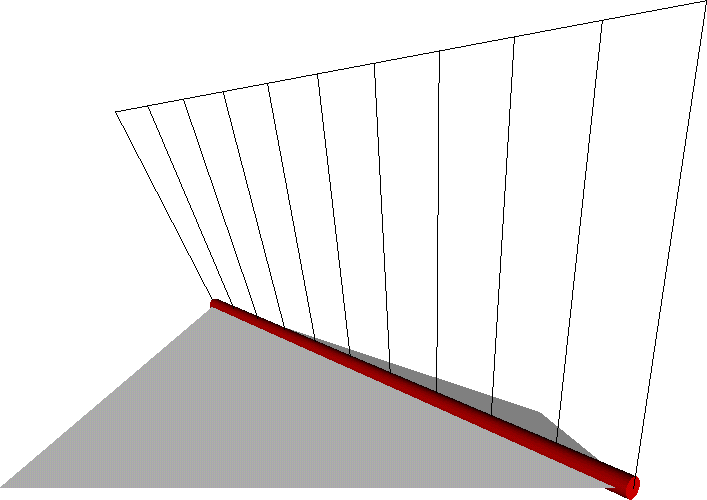
\includegraphics[height=4cm]{../images/ruled_surface_a} &
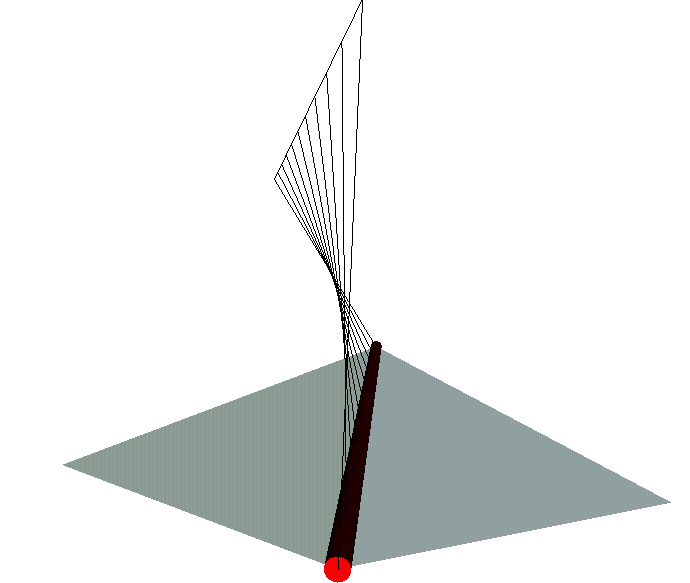
\includegraphics[height=4cm]{../images/ruled_surface_b} &
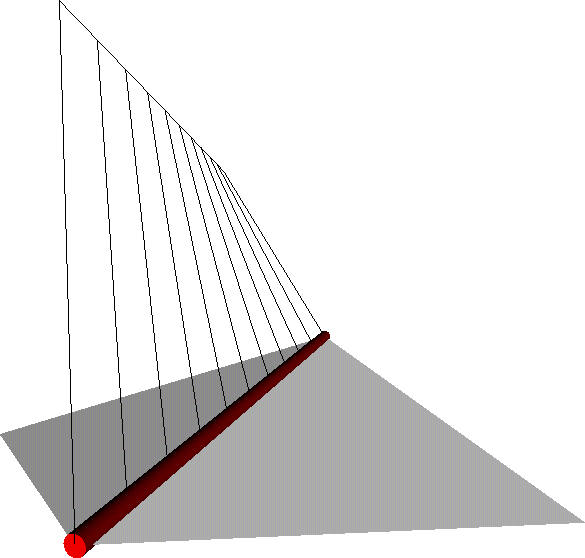
\includegraphics[height=4cm]{../images/ruled_surface_c}
\end{tabular}
\caption[Normal Volume Boundaries]{\label{fig:twistednormals} Normal Volume Boundaries. The boundary of two normal volumes is not planar, but a bilinear ruled surface.}
\end{center}
\end{figure}

It should be noted that the boundaries of a normal volume are not planar. As the boundary is formed by a linear interpolation of the normals at either end, which do not necessarily lie in the same plane, the boundary is in fact a bilinear ruled surface, as shown in figure \ref{fig:twistednormals}. This property does not affect our use of the normal volume at this stage, but will be of importance later on.

\section{\label{sec:scandata:pointtosurface}Point To Surface Mapping}

Once we have defined a volumetric envelope around our mesh surface $M$, we need to define a bijective mapping between an arbitrary point $p$ inside the envelope, and the surface itself. We therefore define a mapping between any point that lies within a normal volume $N_x$, and the related triangle surface $t_x$.

\subsection{\label{sec:scandata:pointtosurface:areal}Areal Coordinates}

\nomenclature{\bf Areal Coordinates}{A coordinate for a point defined by its relation to three or more other points. Each component of the coordinate is a {\it weight} for the corresponding point. The sum of the components is 1.}
Any point $\vec{p}_j \in {\mathbb R}^3$ can be represented as an affine combination of three or more linearly independent points $\vec{p}_0, \vec{p}_1, ..., \vec{p}_n$.

\begin{equation} \label{eqn:barycentric}
\vec{p}_j = \omega_0\vec{p}_0 + \omega_1\vec{p}_1 + ... + \omega_n\vec{p}_n
\end{equation}

The coefficients $(\omega_0, \omega_1, ..., \omega_n)\symbol{areal}$ make up a {\it barycentric coordinate}. Barycentric coordinates are in fact a general form of this type of coordinate, and in the case where the sum of all $\omega_i$ is 1, they are called {\it areal coordinates} \cite{Weisstein99}. If all points $\vec{p}_i$ are coplanar, the resulting point $\vec{p}_j$ will also lie on that plane. This allows us to represent any point $\vec{p}_j$ on the surface of a triangle $t_x$ in this form, by defining an areal coordinate for the point in terms of the triangle vertices $(\vec{v}_a,\vec{v}_b,\vec{v}_c)$.

\begin{equation} \label{eqn:interpolatedpoint}
\vec{p}_j = \omega_a\vec{v}_a + \omega_b\vec{v}_b + \omega_c\vec{v}_c
\end{equation}

\begin{figure}
\begin{center}
\setlength{\unitlength}{0.4cm}
\begin{picture}(20,12)
% triangles
\thicklines
\put(1,6){\line(2,1){12}}
\put(1,6){\line(3,-1){18}}
\put(13,12){\line(1,-2){6}}
% points
\put(1,6){\circle*{0.2}}
\put(13,12){\circle*{0.2}}
\put(19,0){\circle*{0.2}}
\put(11,6){\circle*{0.2}}
% internal lines
\thinlines
\put(1,6){\line(5,0){10}}
\put(13,12){\line(-1,-3){2}}
\put(19,0){\line(-4,3){8}}
% labels
\put(0,6){$\vec{v}_a$}
\put(13.5,12){$\vec{v}_b$}
\put(19.5,0){$\vec{v}_c$}
\put(12,6){$\vec{p}_j$}
\put(14,6){$\omega_a$}
\put(10,4){$\omega_b$}
\put(9,8){$\omega_c$}
\put(2,1){$\omega_a + \omega_b + \omega_c = 1$}
\end{picture}
\caption[Areal Coordinates]{\label{fig:arearatios} Areal coordinates are calculated from area ratios of each sub-triangle and the enclosing triangle.}
\end{center}
\end{figure}

Such an areal coordinate is normally calculated by the use of area ratios, as shown in figure \ref{fig:arearatios}. $\omega_i$ is equal to the ratio of the area of the triangle opposite the vertex to the area of the entire triangle, and can be calculated using the 2D cross product method shown in the following equations.
\begin{eqnarray}
{\cal A} & = & (\vec{v}_b - \vec{v}_a) \times (\vec{v}_c - \vec{v}_a) \\
\omega_a & = & ((\vec{v}_b - \vec{p}_j) \times (\vec{v}_c - \vec{p}_j)) / {\cal A} \\
\omega_b & = & ((\vec{p}_j - \vec{u}_a) \times (\vec{v}_c - \vec{v}_a)) / {\cal A} \\
\omega_c & = & ((\vec{v}_b - \vec{u}_a) \times (\vec{p}_j - \vec{v}_a)) / {\cal A}
\end{eqnarray}

\subsection{\label{sec:scandata:pointtosurface:nvmapping}Normal Volume Mapping}

As the normal volume $N_x$ is defined based on the vertex positions and normals of the triangle $t_x$, any point $\vec{p}_x$ inside the normal volume $N_x$ can be represented as a combination of a point on the surface of the triangle and a multiple $d$\symbol{distance} of the interpolated normal at that point. Combining equations \ref{eqn:interpolatedpoint} and \ref{eqn:interpolatednormals}:
\begin{eqnarray} \label{eqn:pointinvolume}
\vec{p}_x & = & \vec{p}_j + d \vec{n}_j\nonumber \\
          & = & \omega_a\vec{v}_a + \omega_b\vec{v}_b + \omega_c\vec{v}_c + d(\omega_a\hat{n}_a+\omega_b\hat{n}_b+\omega_c\hat{n}_c)
\end{eqnarray}

In order to be able to express a point inside the normal volume $N_x$ in terms of the triangle $t_x$, we therefore calculate the parameters $\omega_a$, $\omega_b$, $\omega_c$ and $d$ for that point. We first define some useful symbols which will aid our derivation.
\begin{eqnarray} \label{eqn:pointsymbols}
\vec{p}_a & = & \vec{v}_a + d\hat{n}_a \nonumber \\
\vec{p}_b & = & \vec{v}_b + d\hat{n}_b \nonumber \\
\vec{p}_c & = & \vec{v}_c + d\hat{n}_c
\end{eqnarray}

Rearranging and rewriting equation \ref{eqn:pointinvolume} in these terms, we have

\begin{equation}
\vec{p}_x = \omega_a\vec{p}_a + \omega_b\vec{p}_b + \omega_c\vec{p}_c
\end{equation}

However, as noted above, $\omega_a + \omega_b + \omega_c = 1$, so we can remove $\omega_c$ from our representation for good, from now on implicitly defining it in terms of the two remaining $\omega$ components.
\begin{eqnarray} \label{eqn:nomoreomegat}
\omega_c & = & 1 - \omega_a - \omega_b \nonumber \\
\vec{p}_x & = & \omega_a\vec{p}_a + \omega_b\vec{p}_b + (1-\omega_a-\omega_b)\vec{p}_c
\end{eqnarray}
This leaves us with a representation in which we can represent any point inside the normal volume $N_x$ using just three components: $\omega_a$, $\omega_b$ and $d$. These are the parameters we need to compute in order to perform our mapping.

\subsection{\label{sec:scandata:pointtosurface:mappingsoln}Mapping Solution}

We can now solve equation \ref{eqn:nomoreomegat} for the three unknown components, $\omega_a$, $\omega_b$ and $d$. We first rearrange, and use the fact that $\vec{a} \times \vec{a} = \vec{0}$ to remove the $\omega_b$ component.
\begin{eqnarray} \label{eqn:pointonplane}
\vec{p}_x-\vec{p}_c & = & \omega_a(\vec{p}_a-\vec{p}_c) + \omega_b(\vec{p}_b-\vec{p}_c) \nonumber \\
(\vec{p}_x-\vec{p}_c) \times (\vec{p}_b-\vec{p}_c) & = & \omega_a((\vec{p}_a-\vec{p}_c) \times (\vec{p}_b-\vec{p}_c))
\end{eqnarray}
\begin{figure}
\begin{center}
\setlength{\unitlength}{0.8cm}
\begin{picture}(10,9)
% triangles
\thicklines
\put(3,2){\line(2,1){4}}
\put(3,2){\line(3,-1){6}}
\put(7,4){\line(1,-2){2}}
\put(1,6){\line(2,1){6}}
\put(1,6){\line(3,-1){9}}
\put(7,9){\line(1,-2){3}}
% points
\put(3,2){\circle*{0.2}}
\put(7,4){\circle*{0.2}}
\put(9,0){\circle*{0.2}}
\put(1,6){\circle*{0.2}}
\put(7,9){\circle*{0.2}}
\put(10,3){\circle*{0.2}}
\put(6,2){\circle*{0.2}}
\put(5,6){\circle*{0.2}}
% normals
\thinlines
\put(3,2){\vector(-1,2){2}}
\put(7,4){\vector(0,1){5}}
\put(9,0){\vector(1,3){1}}
\put(6,2){\vector(-1,4){1}}
% lines
\put(3,2){\line(1,0){3}}
\put(7,4){\line(-1,-2){1}}
\put(9,0){\line(-3,2){3}}
% vertex labels
\put(2,1.5){$\vec{v}_a$}
\put(1,3.5){$d\hat{n}_a$}
\put(0,5.5){$\vec{p}_a$}
\put(6.5,2){$\vec{p}_j$}
\put(5.5,6){$\vec{p}_x$}
\end{picture}
\caption[Normal volume and point-to-surface mapping]{\label{fig:pointtosurface} Normal volume mapping. A point is mapped onto a single triangle.}
\end{center}
\end{figure}
This equation shows that the point $\vec{p}_x$ lies on a plane formed by the three points $\vec{p}_a$, $\vec{p}_b$, and $\vec{p}_c$, as illustrated in figure \ref{fig:pointtosurface}. The left hand side of the equation is equivalent to twice the area of the triangle formed by $\vec{p}_x$, $\vec{p}_b$, and $\vec{p}_c$. The right hand side is twice the area of the original triangle, scaled by the areal coordinate $\omega_a$. The linear relationship between the two areas will hold true for all cases where the four points are coplanar.

We can now use the fact that $(\vec{a} \times \vec{b}) \cdot \vec{a} = 0$ to remove the $\omega_a$ component and leave us with an equation in which the only unknown is $d$.

\begin{equation}
((\vec{p}_x-\vec{p}_c) \times (\vec{p}_b-\vec{p}_c)) \cdot (\vec{p}_a-\vec{p}_c) = 0
\end{equation}

We then expand this, substituting back in equations \ref{eqn:pointsymbols}.
\begin{eqnarray}
((\vec{p}_x-(\vec{v}_c + d\hat{n}_c)) \times ((\vec{v}_b + d\hat{n}_b)-(\vec{v}_c + d\hat{n}_c))) & \cdot & \nonumber \\
((\vec{v}_a + d\hat{n}_a)-(\vec{v}_c + d\hat{n}_c)) & = & 0
\end{eqnarray}

This equation can then be rearranged into a cubic equation in $d$:
\begin{eqnarray} \label{eqn:cubicd}
d^3((\hat{n}_c \times \hat{n}_b) \cdot \hat{n}_a) & + & \nonumber \\
d^2((\hat{n}_c\times \hat{n}_b )\cdot \vec{v}_a + (\hat{n}_c\times \vec{v}_b )\cdot \hat{n}_a & + & \nonumber \\
(\vec{v}_c\times \hat{n}_b)\cdot \hat{n}_a - ((\hat{n}_a - \hat{n}_c)\times(\hat{n}_a - \hat{n}_b))\cdot \vec{p}_x) & + & \nonumber \\
d((\hat{n}_c\times \vec{v}_b)\cdot \vec{v}_a + (\vec{v}_c\times \hat{n}_b)\cdot \vec{v}_a & + & \nonumber \\
(\vec{v}_c\times \vec{v}_b)\cdot \hat{n}_a - ((\hat{n}_a - \hat{n}_c)\times(\vec{v}_a - \vec{v}_b))\cdot \vec{p}_x & - & \nonumber \\
((\vec{v}_a - \vec{v}_c)\times(\hat{n}_a - \hat{n}_b))\cdot \vec{p}_x) & + & \nonumber \\
(\vec{v}_c\times \vec{v}_b)\cdot \vec{v}_a - ((\vec{v}_a - \vec{v}_c)\times(\vec{v}_a - \vec{v}_b))\cdot \vec{p}_x & = & 0
\end{eqnarray}
The roots of this equation can be found using standard methods. Real values of $d$ correspond to potential planes in which the point $\vec{p}_x$ lies. By calculating the $\omega$ coordinates, we can determine which of these planes gives the correct result. Once we have obtained a value for $d$, then we can rearrange equation \ref{eqn:pointonplane} to calculate the corresponding value for $\omega_a$: 

\begin{equation} \label{eqn:omega_a}
\omega_a = \frac{((\vec{p}_x-\vec{p}_c) \times (\vec{p}_b-\vec{p}_c)) \cdot ((\vec{p}_a-\vec{p}_c) \times (\vec{p}_b-\vec{p}_c))}{\|(\vec{p}_a-\vec{p}_c) \times (\vec{p}_b-\vec{p}_c)\|^2}
\end{equation}

We can then rearrange equation \ref{eqn:nomoreomegat} to give us a value for $\omega_b$, completing our parameterisation.

\begin{equation} \label{eqn:omega_b}
\omega_b = \frac{(\vec{p}_x - \vec{p}_c - \omega_a(\vec{p}_a - \vec{p}_c)) \cdot (\vec{p}_b-\vec{p}_c)}{\|(\vec{p}_b-\vec{p}_c)\|^2}
\end{equation}

There may be more than one potential value of $d$ for a mapping, however there should only be one result which gives valid values for $\omega_a$ and $\omega_b$. As the areal coordinates for the point $\vec{p}_j$ should sum to 1, valid results are those which satisfy the following criteria.
\begin{eqnarray}
0 \leq & \omega_a & \leq 1 \nonumber \\
0 \leq & \omega_b & \leq 1 \nonumber \\
0 \leq & \omega_a + \omega_b & \leq 1 \nonumber
\end{eqnarray}

If any of the areal coordinates $\omega_i$ lie outside the range 0..1, $\vec{p}_x$ does not lie inside the volume, and the result is discarded. Otherwise, the result is valid; i.e. $\vec{p}_x$ lies within the normal volume. In these cases, instead of storing $\vec{p}_x$ as a 3D vector, we can store it as the values $\omega_a$, $\omega_b$, and $d$, which represent a re-parameterisation of $\vec{p}_x$ in terms of the triangle $t_x$ to which it has been mapped.

The normal volume mapping presented herein was originally developed by Wei Sun.

\subsection{\label{sec:scandata:pointtosurface:reconstruction}Surface Reconstruction}

The point-to-surface mapping presented above can be used to map an arbitrary point $\vec{p}_x$ onto a triangle surface $t_x$. Once this mapping is achieved, it is a simple matter to reconstruct the original point position from the parameterised version. Expanding equation \ref{eqn:nomoreomegat}, we can see that the process of reconstruction is a simple barycentric interpolation of the values at the triangle vertices.

\begin{equation} \label{eqn:linear}
\vec{p}_x = \omega_a(\vec{v}_a + d\hat{n}_a)+ \omega_b(\vec{v}_b + d\hat{n}_b) + (1-\omega_a-\omega_b)(\vec{v}_c + d\hat{n}_c)
\end{equation}

\subsubsection{\label{sec:scandata:pointtosurface:reconstruction:animation}Animation}

The properties of the normal volume mapping mean that animation of a mapped surface is also simple. As the normal volume in which the point $\vec{p}_x$ is embedded is defined in terms of the triangle geometry, if that geometry is changed, the normal volume space will stretch as appropriate. Points that are parameterised in terms of this space will be deformed along with the space itself. If the geometry of the surface is modified such that vertices of triangle $t_x$ are changed to the new values $(\vec{v}_a', \vec{v}_b', \vec{v}_c')$ and the corresponding vertex normals are modified to $(\hat{n}_a', \hat{n}_b', \hat{n}_c')$, then we can simply apply equation \ref{eqn:linear} with the new values, and we will obtain a modified position for the point $\vec{p}_x'$.

\begin{equation} \label{eqn:rebuilddetail}
\vec{p}_x' = \omega_a(\vec{v}_a' + d\hat{n}_a') + \omega_b(\vec{v}_b' + d\hat{n}_b') + (1-\omega_a-\omega_b)(\vec{v}_c' + d\hat{n}_c')
\end{equation}

As the new vertex position $\vec{p}_x'$ is only dependent on the vertex positions and normals of the triangle $t_x$, points inside $N_x$ will deform evenly, efficiently and seamlessly as the geometry of the triangle is animated.

\section{\label{sec:scandata:creation}Creation of Layered Models}

Having defined methods for the mapping of the control layer to the skeleton, and for the mapping of the detail to control layer, we can now build a complete layered model. The process consists of the capture of the detailed surface data, followed by creation of the control layer. Once the control layer has been created, a skeleton structure can be created and added, and the three layers are then mapped together to create the final layered model which can be animated and rendered as desired.

\subsection{\label{sec:scandata:creation:capture}Data Capture}
\begin{figure}
\begin{center}
\begin{tabular}{cccc}
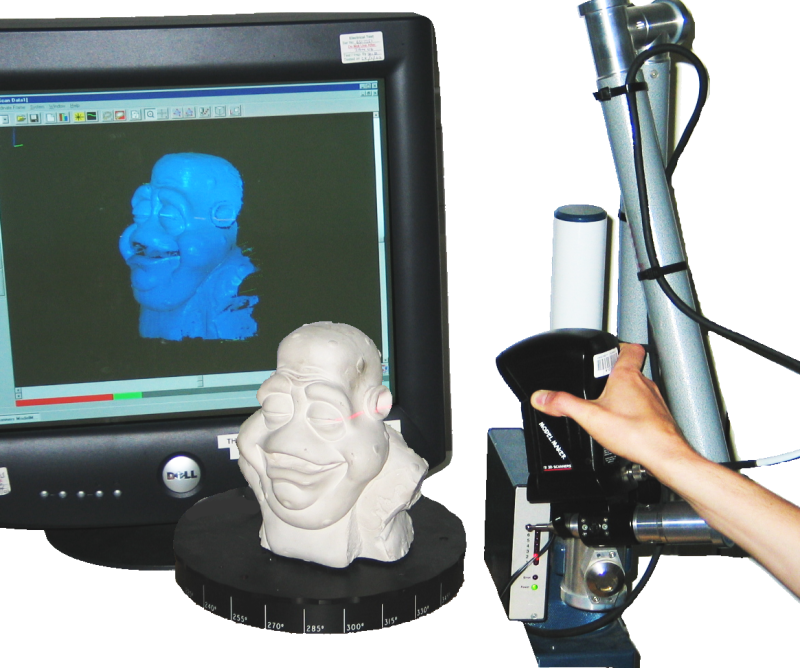
\includegraphics[height=3.8cm]{../images/modelmaker_dino} &
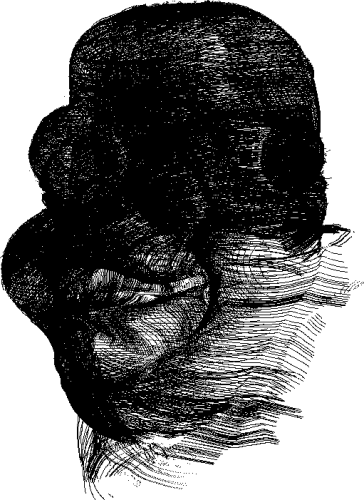
\includegraphics[height=3.8cm]{../images/scandata} &
\includegraphics[height=3.8cm]{../images/decimated_wireframe} &
\includegraphics[height=3.8cm]{../images/decimated_smoothshaded} \\
{\it(a)} & {\it(b)} & {\it(c)} & {\it(d)}
\end{tabular}
\caption[Surface Data Capture]{\label{fig:modelmaker} Surface Data Capture. (a) Data is captured with a laser range scanner. (b) Raw scan data points. (c) A simplified polygonal mesh generated from the scan data. (d) A smoothly shaded view of the polygon mesh.}
\end{center}
\end{figure}
The first stage in the process is the capturing of dense surface data from the object to be modelled. In our case this is carried out using a hand-held laser range sensor, the ModelMaker system from \citet{3DScanners} (see figure \ref{fig:modelmaker}a). The operator moves the scanner over the surface in a straight line, capturing a strip of surface measurements, shown in figure \ref{fig:modelmaker}b, which are then converted into a triangle mesh. As the operator will typically scan a number of strips, a number of polygon meshes will be created. These are then fused together using the method proposed by \citet{Hilton96b}, described above in section \ref{sec:litreview:reconstruction:implicit}. The result of this process is a single, very dense, high-resolution triangle mesh with the same geometry as the original object, a simplified version of which is shown in figure \ref{fig:modelmaker}c. This will be used to form the high-resolution detail layer of our model.

\subsection{\label{sec:scandata:creation:control}Control Layer Creation}
Once we have scanned the surface data which will form the detail layer of our model, we must obtain a control layer mesh. There are a number of properties we require in this mesh, both aesthetic and geometric. Firstly, it should follow the geometry of the detail layer closely. Secondly, it should be of a suitable form for animation; i.e. it should be sufficiently detailed and structured in the right way that all animation we wish to perform is possible. Thirdly, it should be structured in such a way as to minimise the collapse of its normal volumes; this will allow us to define an effective mapping between the layers. We may also wish to enforce a maximum error between the two surfaces, again to create a good mapping. We may also require the mapping from the detail to control layer to be injective, for reasons which will be discussed in chapter \ref{sec:dispmapcreation}.

\begin{figure}
\begin{center}
\begin{tabular}{ccc}
\includegraphics[width=3.5cm]{../images/control_stock} &
\includegraphics[width=3.5cm]{../images/dinohead_control} &
\includegraphics[width=3.5cm]{../images/control_automatic} \\
{\it(a)} & {\it(b)} & {\it(c)}
\end{tabular}
\caption[Control Layer Meshes]{\label{fig:controlmodels} Examples of Control Layer Mesh creation methods (a) Stock model. (b) Interactive creation. (c) Automatic decimation.}
\end{center}
\end{figure}

A control layer mesh can be obtained in a number of different ways. Firstly, it can be a stock model with the same gross shape as the detail layer, and with a structure appropriate for animation, as shown in figure \ref{fig:controlmodels}a. Examples include standard models from \citet{Viewpoint}. 

Alternatively, the control layer can be generated directly from the detail layer. This has the advantage that the control layer is guaranteed to fit the detail layer precisely, and that the error between the two layers will generally be small. The control layer can be generated using either interactive (figure \ref{fig:controlmodels}b) or automatic (figure \ref{fig:controlmodels}c) techniques. Both have their advantages and disadvantages, as we discuss below.

\subsubsection{\label{sec:scandata:creation:control:interactive}Interactive Methods}
\begin{figure}
\begin{center}
\begin{tabular}{cccc}
\includegraphics[width=3.18cm]{../images/eye_dense} &
\includegraphics[width=3.18cm]{../images/eye_polylines} &
\includegraphics[width=3.18cm]{../images/eye_generate} &
\includegraphics[width=3.18cm]{../images/eye_remesh} \\
{\it(a)} & {\it(b)} & {\it(c)} & {\it(d)}
\end{tabular}
\caption[The 3D Scanners Remesh re-modelling process]{\label{fig:remesh}The 3D Scanners Remesh re-modelling process. (a) The scan data is reconstructed into a polygonal mesh. (b) Lines are drawn onto this mesh, splitting the surface into patches. (c) The patches are subdivided equally, with the subdivisions following the surface, which then are used to create a remodelled mesh (d).}
\end{center}
\end{figure}
Using appropriate software, it is possible to interactively create an appropriate control layer, by creating a lower-resolution version of the detail layer. One technique for doing this is demonstrated in figure \ref{fig:remesh}, which shows the process using the Remesh software package from \citet{3DScanners}. 

Once the dense mesh has been scanned into the system, shown in figure \ref{fig:remesh}a, a trained operator can interactively draw {\it polylines} across the surface of the mesh. These are connected to form triangular or quadrilateral patches (see figure \ref{fig:remesh}b), which can then be subdivided by an appropriate factor (see figure \ref{fig:remesh}c). The subdivided patches define the topology of the control mesh, and the geometry is sampled directly from the scanned data. This technique is basically a controlled resampling of the scan data,  which puts the density and location of the sampling points under the control of the modeller.

Interactive control layer generation has the advantage that it is possible for a human operator to design a control layer structure suitable for animation. Polylines can be placed along the natural lines of the detail layer, and more patches can be placed in areas where more mesh flexibility is required. However, the creation of the control mesh takes time, and it is impossible to enforce geometric constraints such as those mentioned above. We would like to keep user interaction to a minimum, so an alternative approach is to use an automatic method of control layer creation.

\subsubsection{\label{sec:scandata:creation:control:automatic}Automatic Methods}

As an alternative to interactive methods, automated methods can be used to generate the control layer mesh. Such methods have an advantage in that we can guarantee that the resulting mesh will satisfy the geometric conditions described above.

Automatic generation methods can guarantee these conditions by carrying out a controlled decimation of the detail layer, using the conditions as a part of the decimation process. While it is difficult to enforce subjective constraints that are easily done by a trained operator using interactive methods, surface properties such as curvature could also be taken into consideration during the decimation process, in order to create a more appropriate mesh structure.

\citet{Collins02} have defined an automatic decimation method based on the work presented herein, which guarantees an injective mapping between the high and low resolution meshes. This method is of particular interest to us, as we require an injective mapping in order to carry out the displacement mapping technique described below in chapter \ref{sec:dispmapcreation}.

This method defines a test which determines if an injective mapping is possible, by comparing the normals of the high and low resolution meshes. If the dot product of these normals is greater than zero, the surfaces are similarly oriented. As long as this condition holds true across the surfaces of both meshes, then an injective mapping is guaranteed. The decimation is performed by collapsing edges in the high-resolution mesh and testing after each collapse that the orientation condition is preserved. The comparison uses the interpolated normal of the low-resolution mesh, as described above for normal volumes. The algorithm can reduce polygon counts by around 99\%, while guaranteeing an injective mapping.

The major problem with this approach is that it will not normally produce models that are suitable for animation. The decimated control mesh is likely to be as unstructured as the detail mesh from which it was generated.

\subsubsection{\label{sec:scandata:creation:control:semiautomatic}Semi-Automatic Methods}

The best results may, in fact, be obtained from a fusion of the two approaches discussed above. A trained operator could create a mesh with a structure suitable for animation, which an automatic process could then refine to enforce the desired geometric properties. This approach is worthy of further research, but is not covered in this thesis.

\subsection{\label{sec:scandata:creation:skeletalmapping}Control Layer to Skeleton Mapping}

Once the control layer has been created, we can fit a skeleton inside it as described in section \ref{sec:skeletalanim:fitting} and perform the mapping between these two layers. If the control and detail layers have radically different geometries (for instance a human body in a different pose), which is possible if a stock control layer is used, we fit the same skeleton structure inside the detail layer. The difference in pose between the skeletons in then used to deform the control layer to fit the detail layer before mapping occurs.

\subsection{\label{sec:scandata:creation:mapping}Detail to Control Layer Mapping}

\begin{figure}
\begin{center}
\begin{tabular}{cc}
\includegraphics[width=6cm]{../images/dinohead_control} &
\includegraphics[width=6cm]{../images/dinohead_detail} \\
{\it (a)} & {\it (b)} \\
\includegraphics[width=6cm]{../images/dinohead_control_colour} &
\includegraphics[width=6cm]{../images/dinohead_mapflat} \\
{\it (c)} & {\it (d)}
\end{tabular}
\caption[Detail layer mapping]{\label{fig:detailmapping} Detail Layer Mapping. (a) Control mesh. (b) Detail Layer. (c) Coloured control mesh. (d) Mapping of detail layer points to control mesh triangles. The triangles on the model shown in (d) are coloured according to the triangle in (c) that their vertices map to. Triangles with vertices that map to more than one control mesh triangle are coloured grey. }
\end{center}
\end{figure}
We must then calculate the mapping between the control and detail layers. Using the method described in section \ref{sec:scandata:pointtosurface}, we perform an exhaustive search, attempting to map each detail layer point to each control layer triangle in turn\footnote{This search could be constrained by taking point and triangle adjacency information into account, but this is not included in our current method.}. A valid result should only be obtained for one control triangle. In the case where more than one valid result is found, for instance in areas of high curvature where normal volumes intersect, the result with the lowest value for $d$ is chosen. This simple distance criterion may not always give the correct mapping however, so other information should also be considered, for instance surface orientation. This issue should also be taken into account during control mesh creation, where it could be checked for and avoided during the automatic decimation process. If $v_d$ represents the number of detail layer vertices, and $t_c$ the number of control layer triangles, the mapping algorithm for a complete mesh has order $O(v_d t_c)$.

Once all detail layer points have been mapped, the original detail layer data can be discarded. The geometry of the detail layer can then be rebuilt from the mapping results as shown in figure \ref{fig:detailmapping}d. The faces of the model are coloured according to which control layer triangle they map to - the coloured control layer is shown in figure \ref{fig:detailmapping}c. Detail layer triangles which have vertices mapping to different control layer triangles are coloured grey.

\subsection{\label{sec:scandata:creation:lmtool}LMTool Interface}

\begin{figure}
\begin{center}
\includegraphics[width=3.5cm]{../images/lmtool_control}
\includegraphics[width=3.5cm]{../images/lmtool_detail}
\includegraphics[width=3.5cm]{../images/lmtool_mapdialog}
\includegraphics[width=3.5cm]{../images/lmtool_mapping}
\caption[LMTool Application Interface.]{\label{fig:lmtool} LMTool Application Interface. The screenshots show the process of loading a control and detail layer, then performing the mapping between the two.}
\end{center}
\end{figure}

During this research, a graphical software application was created to assist in the creation and manipulation of our layered models, called {\it LMTool}. It was developed on a Linux platform, and based on both the AMMA software library \cite{AMMA} created by the CVSSP, and OpenGL \cite{OpenGL} for the 3D graphical display.

LMTool has many functions within it, most of which will be discussed later on in this thesis. At this stage, we are simply interested in the process of creating layered models from a pair of polygon meshes. Upon starting the application, two polygon meshes are loaded. The first is the control layer, shown in figure \ref{fig:lmtool}a. The second is the scanned surface data, shown in figure \ref{fig:lmtool}b, which will be used to create the detail layer of our model. To perform the mapping, a menu option is selected and a dialog is displayed. This dialog allows the user to choose which mapping algorithm should be used\footnote{Various experimental mapping algorithms were used throughout the course of this thesis. All were minor variations on the final version presented here, and will not be discussed further herein.}. Upon pressing ``Execute'', the application then performs the point-to-surface mapping process described in section \ref{sec:scandata:pointtosurface}. The results are then displayed in the window, with the mesh coloured as described in figure \ref{fig:detailmapping}.

LMTool does not presently include skeletal animation capabilities, so is limited to the execution of the mapping process and the rebuilding of mapped detail layers. The control mesh can, however, be manipulated manually within the tool, allowing some rudimentary animation to be carried out. The user can select vertices on the control mesh and drag them around in the window. Some animation using this technique will be shown in section \ref{sec:scandata:results} below.

\section{\label{sec:scandata:results}Results}

\begin{table}
\begin{center}
\begin{tabular}{c|c|c|c|c|c} 
Model & & Cubehead & Monster & Horse & Bunny \\
\hline
			& Vertices & 2215 & 15045  & 48485 & 34876 \\
\raisebox{1.5ex}{Detail}& Triangles & 4042 & 30086  & 96966 & 69535 \\
\hline
  	& Method & Stock & Interactive & Automatic & Automatic \\
Control & Vertices & 8 & 32  & 407 & 487 \\
  	& Triangles & 12 & 60  & 810 & 757 \\
\hline
\end{tabular}
\caption[Model Statistics]{\label{tbl:models} Model Statistics. }
\end{center}
\end{table}

We have tested our mapping algorithm on a number of different models, which are shown in figure \ref{fig:models}. Statistics for the models are shown in table \ref{tbl:models}. The bottom row of the figure shows the results of the mapping for each model. The geometry of the mapped models is rebuilt from the mapped detail layer, but is identical to the original detail layer mesh in every way.

\begin{figure}
\begin{center}
\begin{tabular}{cccc}
\includegraphics[height=3cm]{../images/cubehead_detail} &
\includegraphics[height=3cm]{../images/dinohead_detail} &
\includegraphics[height=3cm]{../images/horse_detail} &
\includegraphics[height=3cm]{../images/bunny_detail} \\
\includegraphics[height=3cm]{../images/cubehead_control} &
\includegraphics[height=3cm]{../images/dinohead_control} &
\includegraphics[height=3cm]{../images/horse_control} &
\includegraphics[height=3cm]{../images/bunny_control} \\
\includegraphics[height=3cm]{../images/cubehead_mapsmooth} &
\includegraphics[height=3cm]{../images/dinohead_mapsmooth} &
\includegraphics[height=3cm]{../images/horse_mapsmooth} &
\includegraphics[height=3cm]{../images/bunny_mapsmooth} \\
{\it (a)} & {\it (b)} & {\it (c)} & {\it (d)} 
\end{tabular}
\caption[Test Models]{\label{fig:models} Test Models. (a) Cubehead. (b) Monster. (c) Horse. (d) Bunny. The top row shows the detail layer mesh, while the middle row shows the control layer. The bottom row shows the reconstructed mapped detail layers, coloured as explained in figure \ref{fig:detailmapping}. }
\end{center}
\end{figure}

\subsection{\label{sec:scandata:results:animation} Animation}

\begin{figure}
\begin{center}
\begin{tabular}{ccc}
\includegraphics[width=3cm]{../images/mapanim_1} &
\includegraphics[width=3cm]{../images/mapanim_2} &
\includegraphics[width=3cm]{../images/mapanim_3} \\
\includegraphics[width=3cm]{../images/mapanim_4} &
\includegraphics[width=3cm]{../images/mapanim_5} &
\includegraphics[width=3cm]{../images/mapanim_6} \\
& (a) &
\end{tabular}
\begin{tabular}{cc}
\includegraphics[width=4cm]{../images/horse_mapanim2} &
\includegraphics[width=4cm]{../images/horse_mapanim3} \\
\includegraphics[width=4cm]{../images/horse_mapanim4} &
\includegraphics[width=4cm]{../images/horse_mapanim5} \\
\multicolumn{2}{c}{(b)}
\end{tabular}
\caption[Detail Layer Animation]{\label{fig:detailanim} Detail Layer Animation. (a) Facial animation of the Monster head, performed by direct manipulation of control mesh vertices. (b) Horse animation, performed by animation of the control mesh in 3D Studio MAX.}
\end{center}
\end{figure}

Figure \ref{fig:detailanim} shows animation of the mapped detail layer, for the Monster and Horse models. By manipulating the control layer mesh, we can perform animation of the complex datasets that make up the detail layer. As the control mesh for a model is animated, the rebuilt detail layer deforms with it. As the normal volumes of the control layer stretch, the normals within them are smoothly interpolated, and the detail layer stretches smoothly across the surface of the polygon.

\section{\label{sec:scandata:conclusion}Conclusion}

In this chapter, we have presented a method of animating densely scanned surface data based on animation of a lightweight control mesh. The method enables animators to use a simplified version of the scanned data for realtime animation planning, which can then be used to automatically perform the same animation on the dense surface in an offline rendering process. Once a suitable control mesh and skeleton structure have been created, the mapping process itself is fully automatic.

The main limitation of this animation method is that it requires us to animate and recalculate the entire detail layer surface, which may consist of a very large number of polygons. This is not a problem for high-quality offline production, which can take as long as is necessary to obtain a realistic result, but it is impossible to use for interactive applications. Therefore, in the next chapter, we introduce an alternative representation of the detail layer surface which will enable us to reconstruct the detail layer surface to an arbitrary levels of detail.


\chapter{\label{sec:dispmapcreation} Displacement Maps}

The layered animation method presented above allows animation of complex datasets, but requires recalculation of every detail layer vertex in each frame in order to render the final surface. While this gives the maximum level of realism and accuracy possible with the layered animation model, it requires too much computation to use for anything other than non-realtime, offline rendering. In this model, only the low-resolution control layer is suitable for real-time rendering. 

Ideally, we would like to be able to regenerate the detailed surface at an arbitrary level of detail, allowing us to control the trade-off between the amount of surface detail and the calculation time required. This would allow us to render the model at any level of detail we like, from a basic model for realtime manipulation, to a full-detail surface for offline rendering. This would allow our representation to be used in many more application areas, from games to film production.

Therefore, we require an alternative representation of the detail layer, which will enable us to choose how much of the surface detail is reconstructed, and in which areas of the model. We can then produce animated reconstructions that are more detailed than the control layer, but can still be rendered in real time. Such a representation may also allow us to edit the detailed surface in a simple manner, and also to compress the detailed surface data into a more compact form.

We require a number of properties for our alternative parameterisation. The most important property is that if we are to work with arbitrary levels of detail, we must be able to obtain the correct value of the detail layer for any point on the control layer, not just those corresponding to detail layer vertices. The parameterisation should also preserve as much detail as possible from the original surface, and animate in the same smooth manner as the detail layer in our original layered animation approach.

We therefore choose to represent the detail layer as a {\it displacement map} defined over the control layer. The displacement map is an error function whose value represents the difference between two surfaces. This error function can be either a vector or scalar field, depending on the required properties. As we only need to encode a single value, i.e. the distance along the surface normal for each point on the control layer, we only require a scalar displacement field. Choosing a scalar-valued field also has advantages in that the representation is more compact, requiring only one parameter per sample point, as opposed to three for a vector field.

If we {\it unwrap} the three-dimensional control layer onto a two-dimensional plane, we can assign the displacement values for the detail layer to points on this 2D plane. The displacement field is sampled at each point on the plane, so that as well as storing displacements for each of the vertices in the original detail layer, we also store values for all points on the control layer mesh in between these vertices. Once the detail layer is encoded in this form, we have much more flexibility in reconstructing the surface detail, as we can choose to recreate an arbitrary part of the surface, including parts that did not exist as vertices in the original detail layer. 

As the error function is scalar, and each point on the 2D plane has only a single value, we can store the displacement map as an image which is mapped to the 3D surface. However, instead of encoding surface colour, the displacement image encodes the scalar error value between our low and high resolution surfaces for each pixel. 

\section{\label{sec:dispmapcreation:overview}Algorithm Overview}

The process of generating a displacement map consists of a number of stages. First, we define a valid mapping from the surface of the 3D control mesh to a 2D image plane. Then, we generate the displacement map by storing the error between the control and detail layers at each point as the value of a pixel on the image plane.

\begin{figure}
\begin{center}
\setlength{\unitlength}{0.4cm}
\begin{picture}(18,12)
% Control Mesh
\thicklines
\put(0,6){\circle*{0.2}}
\put(0,6){\line(1,1){6}}
\put(0,6){\line(2,-1){12}}
\put(6,12){\circle*{0.2}}
\put(6,12){\line(1,-2){6}}
\put(6,12){\line(3,-1){12}}
\put(12,0){\circle*{0.2}}
\put(12,0){\line(3,4){6}}
\put(18,8){\circle*{0.2}}
% T^E
\thinlines
\put(7,5){\line(3,1){3}}
\put(7,5){\line(2,3){2}}
\put(10,6){\line(-1,2){1}}
% T^I
\put(11,8){\line(2,-3){2}}
\put(11,8){\line(3,-1){3}}
\put(13,5){\line(1,2){1}}
\end{picture}
\caption[Internal and External Triangles]{\label{fig:intexttriangles} Internal and External Triangles. The large triangles represent the control mesh. The small detail layer triangle on the left is a member of ${\cal T}^E$, while the one on the right is a member of ${\cal T}^I$.}
\end{center}
\end{figure}

We must calculate displacement values for each pixel in the displacement map. We do this by drawing each detail layer triangle $t \in {\cal T}$ into the displacement map in turn. We can treat each triangle individually, and calculate the displacement map for one detail triangle at a time. For reasons explained below, we must use two separate methods for doing this, depending on whether the detail triangle is contained wholly within one control layer triangle or not.

We therefore divide the set of detail layer triangles ${\cal T}\symbol{triset}$  into two mutually exclusive sets, ${\cal T}^I$ and ${\cal T}^E$. ${\cal T}^I$ represents the set of {\it internal} triangles, which are wholly contained within the normal volume associated with a single control layer triangle, i.e. all their vertices are mapped to the same control triangle as described in section \ref{sec:scandata:creation:mapping}. Conversely, ${\cal T}^E$ represents the set of {\it edge} triangles, which do not fulfil this criterion, and whose vertices map to more than one control layer triangle. This distinction is illustrated in figure \ref{fig:intexttriangles}.

The general process of displacement map creation is summarised in algorithm \ref{alg:dispmapping}, and is explained in detail in the following sections.

\begin{algorithm}[tbp]
\begin{algorithmic}
\IF{Control layer does not have pre-existing texture coordinates.}
	\STATE Generate texture coordinates for control layer
\ENDIF
\FORALL {$t \in {\cal T}$}
	\IF {$t \in {\cal T}^I$}
		\STATE Resample $t$ into the displacement map
	\ELSE
		\FORALL {normal volumes $N \in {\cal N}$ that contain part of $t$}
			\STATE Calculate the geometric intersection ${\cal I} = t \cap N$
			\STATE Resample ${\cal I}$ into the displacement map
		\ENDFOR
	\ENDIF
\ENDFOR
\end{algorithmic}
\caption{\label{alg:dispmapping}Displacement Map Generation}
\end{algorithm}

\section{\label{sec:dispmapcreation:unwrap}Texturing the Control Layer}

In order to generate a displacement map for our high-resolution detail layer, we must first define a bijective mapping from the 3D control layer to a 2D image representation, by defining {\it texture coordinates} for the mesh\footnote{This mapping is one-to-one when each control triangle is considered individually, but not for the mesh as a whole. For instance, an edge in the control mesh may have two locations in the image plane, and a vertex may have any number. The values for all instances of an edge or vertex in the image plane should be the same, however, so this is not a problem.} . If we do not already have manually-defined texture coordinates for the control layer mesh, we must automatically generate this information. We must map each triangle in the control layer to a separate area in the image, into which we will store the displacement values for that triangle.

There are a number of properties we would like in our mapping into the 2D texture domain. Ideally, triangle adjacency should be preserved as much as possible; i.e. triangle which share edges in the mesh should also share them in the image domain. This property makes it easy for the resulting images to be edited as a whole; it would be much harder to edit a displacement map composed of multiple disjointed triangles. We would also like to preserve the relative sizes of the triangles, so that a large triangle is sampled more densely than a small one, allowing us to subdivide it further with a high level of accuracy.

The simplest option for generating texture coordinates is to simply ignore the geometric information in the control mesh, and assign texture coordinates to each triangle in a regular pattern. An example of such as pattern is shown in figure \ref{fig:texcoords}a. As each triangle is considered individually, this method ignores both triangle adjacency and relative size. However, it does guarantee a bijective mapping.

An alternative to the regular mapping above is a {\it cylindrical} mapping \cite{Lengyel02}, shown in figure \ref{fig:texcoords}b. For this method, each mesh vertex is converted into a cylindrical coordinate system whose origin is the centroid of the mesh. The cylindrical coordinate system represents a point $\vec{p}$ as a combination of the parameters $r$, $\phi$ and $y$. $r$ is the straight-line distance from the origin to $\vec{p}$, $||\vec{p}||$. The {\it azimuth} value, $\phi$, is the angle between the plane $x=0$ and $\vec{p}$. The $y$ value has the same meaning as in a standard Cartesian coordinate system, and represents the height above the plane $y=0$. Once these coordinates have been calculated for each point, normalised $\phi$ and $y$ values are used to define 2d coordinates on the image plane. The $r$ coordinate is ignored.

Closely related to the cylindrical method described above is {\it spherical} mapping \cite{Lengyel02}. This is identical to the cylindrical case, except that the $y$ coordinate is replaced by $\theta$, the {\it polar angle}. This represents the angle between the vector $\vec{p}$ and the plane $y=0$. The $\phi$ and $\theta$ coordinates are normalised to the range 0 to 1 and used as a 2D coordinate in the image plane. Spherical mapping is shown in figure \ref{fig:texcoords}c.

While the two methods above preserve some adjacency and size information, they do not guarantee a bijective mapping, as it is possible for triangles to overlap when mapped to the enclosing cylinder or sphere. We can generate a map that give us the best features of the previous three methods by using the {\it pelting} method, proposed by \citet{Piponi00}, which is illustrated in figure \ref{fig:texcoords}d. In this method, a set of mesh edges are defined as seams, along which the mesh will be split. These seams are then ``stretched'' out, until the mesh is flattened, at which point texture coordinates can be simply inferred from the coordinates of the vertices. However, one drawback of this method is that relative sizes of triangles in the original mesh are very difficult to preserve or control in any predictable way.

\begin{figure}
\begin{center}
\begin{tabular}{cccc}
\includegraphics[width=3.2cm]{../images/texcoord_reg} &
\includegraphics[width=3.2cm]{../images/texcoord_cyl} &
\includegraphics[width=3.2cm]{../images/texcoord_sph} &
\includegraphics[width=3.2cm]{../images/texcoord_plt} \\
{\it (a)} & {\it (b)} & {\it (c)} & {\it (d)}
\end{tabular}
\caption[Texturing Methods]{\label{fig:texcoords} Texturing Methods, generated for the Monster head control model. (a) Regular. (b) Cylindrical mapping. (c) Spherical mapping. (d) Pelting.}
\end{center}
\end{figure}

In this research, where pre-existing texture coordinates were unavailable, we have used a mixture of the regular and pelting methods for different models. In cases where it is desirable to preserve triangle adjacency, for instance for hand editing of the displacement map, the pelting method can be used. However, this method requires user intervention to define seams. In most cases the regular pattern is used to automatically define a planar mapping, as it requires no user input. Although this method does not preserve triangle area, it will result in more detail being stored for smaller control layer triangles. Seeing as smaller triangles will generally be present in areas of high curvature and detail, this allows us to store more information for these areas, which will lead to better visual quality. If we do not wish to have this effect, an adaptive version can be used which preserves triangle area.

\section{\label{sec:dispmapcreation:points}Drawing Points}

\begin{figure}
\begin{center}
\begin{tabular}{ccc}
\includegraphics[width=4cm]{../images/cubehead_detail} &
\includegraphics[width=4cm]{../images/cubehead_control_colour} &
\includegraphics[width=4cm]{../images/cubehead_mapflat} \\
{\it (a)} & {\it (b)} & {\it (c)}
\end{tabular}
\begin{tabular}{cc}
\includegraphics[width=5.9cm]{../images/cubehead_bigpoints} &
\includegraphics[width=5.9cm]{../images/cubehead_noedges} \\
{\it (d)} & {\it (e)} \\
\includegraphics[width=5.9cm]{../images/cubehead_full} &
\includegraphics[width=5.9cm]{../images/cubehead_folds} \\
{\it (f)} & {\it (g)}
\end{tabular}
\caption[Displacement Mapping]{\label{fig:dispmap} Displacement Mapping Overview. (a) Original Mesh. (b) Control Mesh. (c) Mapping results. (see figure \ref{fig:detailmapping} for explanation of colour scheme). (d) Displacement map, points only. (e) Internal Triangles Filled. (f) Edge Triangles Filled. (g) Surface Folding. The displacement maps have been colourised to enhance the visibility of details.}
\end{center}
\end{figure}

In order to generate a displacement map representing the detail layer, we need to calculate the value of the error function across the surface of the control layer. To do this, we need to resample the 3D mesh from the detail layer into displacement values in a 2D image which is mapped to the control layer as described above. Conveniently, we have a simple way to do this from our previous calculations for layered animation. As explained in section \ref{sec:scandata:pointtosurface}, we represent each mapped detail layer vertex $\vec{p}$ as a set of four coordinates, $\omega_a$, $\omega_b$, $d$, and a control triangle index $t$.

This parameterisation will convert easily into an image-based format. If the control triangle $t_x$ has texture coordinates $\vec{u}_x\symbol{texcoord}$ for each of its vertices $\vec{v}_x$, then $\omega_a$ and $\omega_b$, the mapped coordinates of a detail layer vertex $\vec{p}$, define $\vec{u_{p}}$, a 2D position in the image for that point, as shown in equation \ref{eqn:imgpoint}.

\begin{equation} \label{eqn:imgpoint}
\vec{u_{p}} = \omega_a\vec{u}_a + \omega_b\vec{u}_b + (1-\omega_a-\omega_b)\vec{u}_c
\end{equation}

The distance value $d$ is then assigned to the pixel at this point. For the mesh shown in figure \ref{fig:dispmap}a (for which texture coordinates were assigned manually), the result of this process is shown in figure \ref{fig:dispmap}d. Each point in the image represents a point in the detail layer, and the colour of each point represents its distance. The texture image itself is composed of real-valued pixels at this stage, as we want to avoid losing any detail through quantisation until absolutely necessary.

\section{\label{sec:dispmapcreation:triangles}Filling Triangles}

While drawing the detail layer vertices into our displacement map may accurately encode all the vertex information from the detail layer, topological information (i.e. the mesh connectivity) is lost. When we create a displacement map, although we are not interested in the exact topology of the mesh, we do wish to preserve the exact shape of the detail layer surface. Therefore, rather than drawing individual points into the displacement map as described above, we calculate the displacement map over the {\it entire} detail layer surface by drawing complete detail layer triangles into the map.

Our triangle drawing method falls into two parts, that used for ${\cal T}^I$, and that used for ${\cal T}^E$. For each triangle $t \in {\cal T}^I$, we calculate a mapped triangle in the 2D image. This is done by mapping each of the detail layer triangle vertices into the image plane, creating a set of 2D coordinates for the vertices. These mapped points then form a triangle in the image which corresponds to the mapping of the detail layer triangle. The displacement values at the triangle vertices are taken directly from the detail layer mapping, but we must also calculate displacement values for every pixel inside the 2D mapped triangle.

\begin{figure}
\begin{center}
\includegraphics[width=6cm]{../images/raster}
\caption[Triangle Rasterisation]{\label{fig:raster} Triangle rasterisation identifies which pixel centres lie inside the triangle.}
\end{center}
\end{figure}

First of all, the mapped triangle is {\it rasterised}, a process in which we calculate which pixel centres lie inside the triangle boundary (see figure \ref{fig:raster}a). A set of areal coordinates $(\omega_a ,\omega_b ,\omega_c)$ are then calculated for each pixel centre $\vec{p}_x$ which lies inside the triangle $\triangle{\vec{u}_a,\vec{u}_b,\vec{u}_c}$. The areal coordinates are calculated using the area ratio method described in section \ref{sec:scandata:pointtosurface:areal}.

We can then use the areal coordinate for each pixel to calculate a displacement value $d_p$ for that pixel by barycentric interpolation of the displacement values $d_x$ at the corners $\vec{u}_x$ of the mapped triangle, which are obtained from the original point-to-surface mapping. 

\begin{equation} \label{eqn:pixeldisp}
d_p = \omega_a d_a + \omega_b d_b + \omega_c d_c
\end{equation}

In this way, each pixel whose centre lies within the triangle is filled with the appropriate interpolated displacement value. The results of this filling are shown in figure \ref{fig:dispmap}e. Note that at this stage, only triangles in ${\cal T}^I$ are filled.

A more efficient scanline conversion algorithm could be used instead of the per-pixel linear interpolation, but we choose to use the per-pixel calculation in the interests of keeping the algorithms generalised.

\subsection{\label{sec:dispmapcreation:triangles:approx}Linear Approximation}

\begin{figure}
\begin{center}
\begin{tabular}{cc}
\includegraphics[height=3.5cm]{../images/approx_a} &
\includegraphics[height=3cm]{../images/approx_b} \\
{\it (a)} & {\it (b)} \\
\includegraphics[height=3.5cm]{../images/approx_c} &
\includegraphics[height=3cm]{../images/approx_d} \\
{\it (c)} & {\it (d)} \\
\includegraphics[height=3.5cm]{../images/approx_e} &
\includegraphics[height=3cm]{../images/approx_f} \\
{\it (e)} & {\it (f)}
\end{tabular}
\caption[Triangle Filling Approximation]{\label{fig:approximation} Triangle Filling Approximation. Examples shown in 2D for clarity. (a) A detail layer triangle maps to a control layer triangle. (b) d does not vary linearly. (c) Comparatively small triangles map to a control layer triangle. (d) Approximation error is reduced as triangles become smaller. (e) Sampling and quantisation errors. (f) Linear approximation. }
\end{center}
\end{figure}

The linear interpolation across detail layer triangles, described above, does not in fact represent the surface shape with full accuracy, but includes a linear approximation which simplifies calculation of the displacement map.

Figure \ref{fig:approximation}a shows 2D representation of a detail layer triangle, of a similar size to the control layer triangle it is being mapped to. Due to the shape of the normal volume and the mapping between layers, the distance between each point on the surface of the detail triangle and its mapping to the control surface will vary across the triangle, even if the two are parallel. 

Figure \ref{fig:approximation}b shows how the $d$ value varies across the surface. The distance is not only related to the position of the detail layer surface, but also to the angle formed between the mapping vector and the control layer triangle at the point in question. If we represent the displacement values across a triangle by a linear interpolation, errors will be introduced as we fail to capture the curvature shown in figure \ref{fig:approximation}b correctly.

The situations shown in figure \ref{fig:approximation}a will be rare, as detail layer triangles will normally be substantially smaller than the control layer triangles that they are mapped to, as shown in figure \ref{fig:approximation}c. In this case, the surface is formed of many detail layer triangles across the surface of the control triangle, each of which is curved in normal volume space as shown in figure \ref{fig:approximation}d. As they are explicitly calculated, the displacement values at vertices on the detail layer will always be correct, meaning that the error introduced by our linear interpolation is reduced, as the surface is ``fixed'' to the correct displacement value at each vertex. Our linear approximation will lie much closer to the actual surface shape as shown in figure \ref{fig:approximation}f.

The errors introduced by this linear approximation are acceptable however, as they are only significant at certain scales, and in the remainder of cases will be insignificant compared to other sources of error. Firstly, errors will only be significant when a detail layer triangle fills a large proportion of the normal volume in which it lies. As we are generally mapping very dense meshes to much simpler control layers, this should be an exceptional case and occur only rarely. Secondly, processes which take place after the creation of the displacement map, for instance quantisation for file storage, or resampling for detail layer reconstruction, will introduce further errors and approximations which will dominate over the small scale of these linear approximation errors.

For these reasons, and because it simplifies the method and reduces computation time during map creation, we accept this linear approximation as part of our method. It would be entirely possible to remove this error by using a more complex method of triangle-filling, if it became necessary to remove such errors for any particular application. For instance, the errors may become visible in a highly detailed rendering, or under strong specular lighting which may cause the surface to appear dimpled.

\section{\label{sec:dispmapcreation:edges}Dealing with Edge Triangles}
\begin{figure}
\begin{center}
\begin{tabular}{cccc}
\includegraphics[height=5cm]{../images/edgetriangle_b} &
\includegraphics[height=5cm]{../images/edgetriangle_a} \\
{\it (a)} & {\it (b)} \\
\includegraphics[height=5cm]{../images/edgetriangle_c} &
\includegraphics[height=5cm]{../images/edgetriangle_d} \\
{\it (c)} & {\it (d)}
\end{tabular}
\caption[Edge Triangles]{\label{fig:edgetriangles} Edge Triangles that lie across normal volume boundaries may become non-triangular when projected to a 2D plane.}
\end{center}
\end{figure}
\begin{figure}
\begin{center}
\includegraphics[width=8cm]{../images/edgetris}
\caption[Edge Cases]{\label{fig:edgecases} Edge Cases. A selection of the possible configurations of the intersection between a control triangle and a detail layer triangle. The area that must be filled is shaded.}
\end{center}
\end{figure}
The method described above suffices for generating displacement map data for triangles in ${\cal T}^I$. However, for those triangles in ${\cal T}^E$, whose vertices map to two or more control mesh triangles, the situation becomes more complex. Even though it is the case that for triangles in ${\cal T}^I$, a triangle will remain triangular when mapped to the 2D image, it is not the case for edge triangles. 

A triangle is mapped linearly inside each normal volume onto the appropriate control triangle. However, adjacent normal volumes will have different mapping properties. This means that if a detail layer triangle crosses a normal volume boundary (as shown in figure \ref{fig:edgetriangles}a), the linear mapping of the triangle will have different parameters on either side of the boundary. The triangle will therefore not remain triangular when mapped to the image plane, as shown in figure \ref{fig:edgetriangles}b.  Therefore, we have to treat the mapping to each control triangle entirely separately, even in cases where edges are shared in the image plane.

For each triangle $t_e \in {\cal T}^E$, we separately calculate its projection into each triangle whose normal volume it crosses. This is not limited to those triangles which its vertices map to, as it may completely cross a normal volume without any of its vertices mapping to the appropriate control triangle. The intersection can take many shapes, some examples of which are shown in figure \ref{fig:edgecases}. Detecting all of the potential cases and filling the displacement map with the appropriate values can be a complex process. This section will discuss the methods we have used for this purpose.

\subsection{\label{sec:dispmapcreation:edges:virtual}Virtual Corner Points}

Initially, in an attempt to avoid calculating the sections of the detail triangle inside each normal volume, a class of drawing methods were explored that involved extending the point-to-surface mapping beyond the normal volume boundary. In order to draw a point into the image plane, we need to calculate its $\omega_a$, $\omega_b$ and $d$ coordinates for the control triangle currently being drawn. In these methods, we calculate these parameters for all detail layer points that are used by an edge triangle, including those that were not originally mapped to the control triangle in question. These calculated points are referred to herein as {\it virtual corner points}.

There were a number of problems with these methods, however. The mapping outside the normal volume proved to be highly unstable, some methods involved time-consuming searches, and all of the methods resulted not in a general algorithm for drawing, but instead a large number of special cases, each of which had to be implemented separately. Therefore, alternative approaches were explored, involving explicit calculation of the triangle sections inside each normal volume. 

%The virtual corner point methods are explained in more detail in appendix \ref{sec:edgemethods}, as although they are not directly related to the final method used, they may still be of some interest. 

\subsection{\label{sec:dispmapcreation:edges:intersection}Intersection Calculation}

If we are to calculate the shape of edge triangles, we must calculate the intersections between the edges of the detail layer edge triangle, and the normal volume boundary of the control triangle we wish to draw it into. However, this is not a simple operation, because the boundaries of the normal volume are not planar, but bilinear ruled surfaces, as mentioned in section \ref{sec:scandata:normalvolume:boundaries}. We therefore use the following method to calculate the intersections with this surface.

Any point $\vec{r}_e$ which lies on an edge of a detail layer triangle can be defined as shown in equation \ref{eqn:intersect_edge}, where $\vec{p}_0$ and $\vec{p}_1$ are the vertices at either end of the detail triangle edge in question, and , and $0 \leq \kappa \leq 1$.

\begin{equation} \label{eqn:intersect_edge}
\vec{r}_e = \kappa\vec{p}_0 + (1-\kappa)\vec{p}_1
\end{equation}

In a similar way, a point $\vec{r}_b$ which lies on a normal volume boundary can be defined as shown in equation \ref{eqn:intersect_boundary}. $\hat{n}_x$ is the surface normal at the control triangle vertex $\vec{v}_x$, $\vec{v}_0$ and $\vec{v}_1$ represent the control triangle vertices at the either end of the normal volume boundary we are testing, and $0 \leq \lambda \leq 1$.

\begin{equation} \label{eqn:intersect_boundary}
\vec{r}_b = \lambda\vec{v}_0 + (1-\lambda)\vec{v}_1 + d(\lambda\hat{n}_0 + (1-\lambda)\hat{n}_1)
\end{equation}

As the intersection point will lie on both the detail triangle edge and the normal volume boundary, the intersection point $\vec{r} = \vec{r}_e = \vec{r}_b$.

Combining equations \ref{eqn:intersect_edge} and \ref{eqn:intersect_boundary} gives us a single equation describing the intersection point, in terms of the unknown values $\lambda$, $\kappa$, and $d$. This formulation is illustrated in figure \ref{fig:intersection}.

\begin{equation} \label{eqn:intersect_combined}
\vec{r} = \kappa\vec{p}_0 + (1-\kappa)\vec{p}_1 = \lambda\vec{v}_0 + (1-\lambda)\vec{v}_1 + d(\lambda\hat{n}_0 + (1-\lambda)\hat{n}_1)
\end{equation}

\begin{figure}
\begin{center}
\setlength{\unitlength}{0.5cm}
\begin{picture}(14,12)
% Points
\put(0,4){\circle*{0.2}}
\put(6,10){\circle*{0.2}}
\put(8,2){\circle*{0.2}}
\put(14,8){\circle*{0.2}}
\put(4,5){\circle*{0.2}}
\put(7,6){\circle*{0.2}}
\put(10,7){\circle*{0.2}}
% Lines
\thinlines
\put(0,4){\line(1,1){6}}
\put(6,10){\line(4,-1){8}}
\put(0,4){\line(4,-1){8}}
\put(8,2){\line(1,1){6}}
\put(6,10){\line(1,-4){2}}
\put(4,5){\line(3,1){6}}
% Normals
\put(6,10){\vector(1,1){2}}
\put(8,2){\vector(-1,-2){1}}
% Labels
\put(3,4.5){$\vec{p}_0$}
\put(10.5,7){$\vec{p}_1$}
\put(5,10){$\vec{v}_0$}
\put(8,1){$\vec{v}_0$}
\put(8,11){$\hat{n}_0$}
\put(6,0){$\hat{n}_1$}
\put(7.5,5.5){$\vec{r}$}
\put(5,5.75){$\kappa$}
\put(7,7.5){$\lambda$}
\end{picture}
\caption[Intersection Calculations]{\label{fig:intersection} Intersection Calculations. Parameters used in the calculation of the intersection point $\vec{r}$ between a line segment and a normal volume boundary. }
\end{center}
\end{figure}

This formula can then be then solved for the three unknowns, $\lambda$, $\kappa$ and $d$, using the following method. First, we define some useful symbols:
\begin{eqnarray}
\vec{p}_{01} & = & \vec{p}_0 - \vec{p}_1 \nonumber \\
\vec{v}_{01} & = & \vec{v}_0 - \vec{v}_1 \nonumber \\
\vec{n}_{01} & = & \hat{n}_0 - \hat{n}_1 \nonumber
\end{eqnarray}

Rearranging equation \ref{eqn:intersect_combined}:

\begin{equation} \label{eqn:intsolv0}
\vec{p}_1 + \kappa\vec{p}_{01} = \vec{v}_1 + d\hat{n}_1 + \lambda(\vec{v}_{01}+d\vec{n}_{01})
\end{equation}

Using the facts that $\vec{a} \times \vec{a} = \vec{0}$ and $d\vec{a} \times \vec{b} = d(\vec{a} \times \vec{b})$, we now take the cross product of both sides with $\vec{p}_{01}$ in order to remove the $\kappa$ component:

\begin{equation}
\vec{p}_1 \times \vec{p}_{01} = (\vec{v}_1 + d\hat{n}_1) \times \vec{p}_{01} + \lambda(\vec{v}_{01}+d\vec{n}_{01}) \times \vec{p}_{01}
\end{equation}
\begin{equation} \label{eqn:intsolv1}
(\vec{p}_1 - \vec{v}_1 - d\hat{n}_1) \times \vec{p}_{01} = \lambda(\vec{v}_{01}+d\vec{n}_{01}) \times \vec{p}_{01}
\end{equation}

We now use the property that $(\vec{a} \times \vec{b}) \cdot \vec{a}  = 0$ to remove $\lambda$ from the equation, leaving only $d$ to solve for.

\begin{equation}
((\vec{p}_1 - \vec{v}_1 - d\hat{n}_1) \times \vec{p}_{01}) \cdot (\vec{v}_{01}+d\vec{n}_{01}) = 0
\end{equation}
\begin{eqnarray} \label{eqn:intsolv2} 
d^2((\hat{n}_1 \times \vec{p}_{01}) \cdot \vec{n}_{01})  & + & \nonumber \\
d((\hat{n}_1 \times \vec{p}_{01} \cdot \vec{v}_{01}) + (\vec{v}_1 \times \vec{p}_{01} \cdot \vec{n}_{01}) - (\vec{p}_1 \times \vec{p}_{01} \cdot \vec{n}_{01})) & + & \nonumber \\
(\vec{v}_1 \times \vec{p}_{01} \cdot \vec{v}_{01}) - (\vec{p}_1 \times \vec{p}_{01} \cdot \vec{v}_{01}) & = & 0
\end{eqnarray}

Equation \ref{eqn:intsolv2} is a quadratic in $d$, and so can be solved using standard methods. The real roots of this equation represent the value of $d$ for potential intersection points. We can now use each possible value of $d$ to calculate possible values for $\lambda$ and $\kappa$. First of all, we can rearrange equation \ref{eqn:intsolv1} for $\lambda$:

\begin{equation} \label{eqn:lambda}
\lambda = \frac{((\vec{p}_1 - \vec{v}_1 - d\hat{n}_1) \times \vec{p}_{01}) \cdot (\vec{v}_{01}+d\vec{n}_{01} \times \vec{p}_{01})}{\|(\vec{v}_{01}+d\vec{n}_{01} \times \vec{p}_{01})\|^2}
\end{equation}

We can then rearrange equation \ref{eqn:intsolv0} to calculate the corresponding value of $\kappa$.

\begin{equation} \label{eqn:kappa}
\kappa = \frac{(\vec{v}_1 + d\hat{n}_1 + \lambda(\vec{v}_{01}+d\vec{n}_{01}) - \vec{p}_1) \cdot \vec{p}_{01}}{\|\vec{p}_{01}\|^2}
\end{equation}

After the calculation is complete, we can discard some potential solutions, as they are outside the desired range. As mentioned above, both $\lambda$ and $\kappa$ must lie between 0 and 1 for the intersection to be valid. The above method may yield results outside that range, in which case they are discarded.

This intersection calculation was developed by Gordon Collins.

\subsection{\label{sec:dispmapcreation:edges:polygon}Polygon Creation}

Once we can detect intersection points between detail layer edges and normal volume boundaries, we can use this information to calculate the exact geometric intersection of the detail triangle and all of the normal volumes in which it lies. Due to the nature of the intersection method, the mapping of this triangle to the control triangle is performed in the same operation as the intersection calculation, so a 3D intersection is never calculated, and the results of the calculation enable us to draw the displacement map directly.

To draw a detail layer triangle into the area of a displacement map  corresponding to a control layer triangle, we calculate a polygon with up to six sides (as shown in figure \ref{fig:edgecases}), which represents the geometric intersection of the detail layer triangle and the normal volume of the control layer triangle. Each point in the polygon is represented by a 2D image plane coordinate, and an associated displacement value. The problem of filling such an arbitrary polygon is discussed below in section \ref{sec:dispmapcreation:edges:filling}.

To build this polygon, we treat each edge of the detail layer triangle in turn. Firstly, we examine the starting vertex of the edge. If the vertex maps to the current control triangle, we add the texture coordinate of the vertex to the polygon, along with its associated displacement value. Then, we examine the ending vertex of the edge. If this also maps, we add it to the polygon as before and proceed to the next edge. Otherwise, we detect intersections between the edge and all boundaries of the normal volume. In this case, there should be only one in the correct range. We add this intersection to the polygon. Its texture coordinate values are interpolated from the end points of the normal volume boundary using the $\lambda$ result of the intersection calculation above. The displacement value, $d$, for the point is obtained directly from the solution to the intersection calculation.

If the starting vertex does not map to the current control triangle, we proceed directly to the calculation of the intersection point. In this case, we can obtain either 0, 1 or 2 results. If there are no results, we proceed directly to the next detail edge - this edge does not cross the normal volume. Otherwise, both intersections are added to the polygon as before, in order of increasing $\kappa$ (which corresponds to a distance along the detail triangle edge).

The only addition to this comes when an incoming edge is detected (i.e. the start point is outside the volume, and intersections are found). In this case we must detect whether the last outgoing edge was on the same side of the normal volume. If not, then we must include all corners of the control triangle between the two edges in our polygon. This involves explicitly calculating a displacement value for the corner point, by using a ray/triangle intersection method.

Once we can draw into a single control triangle, it is a simple matter to draw into many. Starting with each corner point, we maintain a {\it todo} list of normal volumes (identified by their associated control triangle) that we know the detail layer triangle crosses. For each of these, we carry out the method described above. If we detect that the triangle intersects a normal volume boundary, then the normal volume on the other side of that boundary is added to the {\it todo} list. Once drawing is complete in a normal volume, then that volume is added to a {\it done} set. Then, the next volume on the {\it todo} list is processed, as long as it is not in the {\it done} set. Using this method, we will walk around the control layer mesh until the entire detail triangle surface has been drawn into the displacement map.

\begin{algorithm}[tbp]
\begin{algorithmic}
\STATE add detail layer vertex mappings to control triangle todo list
\FORALL { triangle $t$ in todo list}
	\FORALL {edge $e_i \in {\cal E}$ }
		\IF {$v_i$ maps to this control triangle}
			\STATE append $v_i$ to the corner list
			\IF {$v_{i+1}$ does not map to this control triangle}
				\STATE detect intersections between $e_i$ and normal volume boundaries
				\STATE sort intersections into order of lowest $\kappa$
				\STATE append first intersection to corner list
				\STATE {\em LastBoundary} $\Leftarrow$ intersected boundary
				\IF {triangle over intersected boundary is not on done list}
					\STATE add triangle over intersected boundary to todo list
				\ENDIF
			\ENDIF
		\ELSE
			\STATE detect intersections between $v_i$ and normal volume boundaries
			\IF {there are any intersections}
				\STATE sort intersections into order of lowest $\kappa$
				\IF {intersected boundary $\neq$ {\em LastBoundary}}
					\STATE append all control triangle corners between this boundary and the last to the corner list
				\ENDIF
				\STATE append the first intersection to the corner list
				\IF {$v_{i+1}$ does not map to this control triangle}
					\STATE append the second intersection to the corner list
					\STATE {\em LastBoundary} $\Leftarrow$ intersected boundary
					\IF {triangle over intersected boundary is not on done list}
						\STATE add triangle over intersected boundary to todo list
					\ENDIF
				\ENDIF
			\ENDIF
		\ENDIF
	\ENDFOR
	\STATE add $t$ to done list
\ENDFOR
\end{algorithmic}
\caption{\label{alg:polygoncreation}Polygon Generation}
\end{algorithm}

The complete process is summarised in algorithm \ref{alg:polygoncreation}.

\subsection{\label{sec:dispmapcreation:edges:filling}Filling of Non-Triangular Polygons}

It is simple to interpolate values across a triangular region, as explained in section \ref{sec:dispmapcreation:triangles}, but this barycentric interpolation method does not extend directly to polygons with more than 3 sides, as it is not a simple matter to calculate areal coordinates for arbitrary polygons. However, \citet{Meyer02} describe a simple method of generalising areal coordinates to irregular convex polygons, which we can use to fill our clipped triangles. 

This method calculates an areal coordinate for every vertex of an irregular polygon, and preserves the properties found in standard areal coordinates for triangles. A point inside the polygon is represented as an affine combination of the vertices weighted by their areal components, and the sum of all the areal coordinates is 1 for a point inside. The parameterisation is also continuous in all its derivatives, guaranteeing smoothness of the interior under animation of the polygon vertices.

To obtain the $i$th areal coordinate for a point $\vec{p}_x$, we use the formulation shown in equation \ref{eqn:nontriareals}. $\vec{v}_i$ represents the $i$th vertex of the enclosing polygon.
\begin{eqnarray}
\label{eqn:nontriareals}
\vec{v}_p & = & \vec{p}_x - \vec{v}_i \nonumber \\
\vec{v}_- & = & \vec{v}_{i-1} - \vec{v}_i \nonumber \\
\vec{v}_+ & = & \vec{v}_{i+1} - \vec{v}_i \nonumber \\
\theta_- & = & \frac{\vec{v}_- \cdot \vec{v}_p}{\| \vec{v}_- \times \vec{v}_p \|} \nonumber \\
\theta_+ & = & \frac{\vec{v}_+ \cdot \vec{v}_p}{\| \vec{v}_+ \times \vec{v}_p \|} \nonumber \\
\omega_i & = & \frac{\theta_- + \theta_+}{\| \vec{v}_p \| ^2}
\end{eqnarray}

The calculated areal coordinates are then used to calculate the distance value $d_x$ at $\vec{p}_x$ in a similar way to that for triangle filling. $d_i$ represents the distance value at $\vec{v}_i$.

\begin{equation}
\label{eqn:polygonfilling}
d_x = \sum_{i=1}^n \omega_id_i
\end{equation}

\section{\label{sec:dispmapcreation:raycasting}Raycasting}

There is an alternative method of generating the displacement map from that presented above, involving {\it raycasting}. Once the texture coordinates are generated for the control mesh, this method would calculate the 3D position of each pixel in the displacement map on the surface of the control layer. A ray would then be cast along the interpolated surface normal at that point, and any intersections with the detail layer found directly. The distance between the control layer point and the detail layer intersection point would then be stored in the displacement map. 

This technique is perfectly valid, and simpler than the one we present above. It also avoids the linear approximation problem noted in section \ref{sec:dispmapcreation:triangles:approx}, giving a more accurate result. However, one advantage of our approach is that a raycasting approach would need to be specifically designed to cope with holes in the detail mesh, as well as boundaries and so on. Our approach avoids this, as it calculates displacements for each point on the detail mesh, not for each point on the control mesh.

Another advantage of our method is that it should be faster to execute. This is because a raycasting approach must search for intersections between the ray and the detail layer by testing each detail layer triangle in turn. Our approach uses existing mapping results, and fills pixel values in the displacement map directly from these, with no searching required. This implies that the triangle filling method has a lower order than the raycasting method, making it more efficient.

\section{\label{sec:dispmapcreation:folding}Surface Folding}

One problem with scalar-valued displacement maps is that if the mapping from high resolution model to low resolution control layer is non-injective, data loss can occur since the mapping is no longer invertible. If the high resolution model folds over itself inside the normal volume of a single control triangle, a single point on the surface of that control triangle will have more than one possible displacement value. This is an inherent limitation in the displacement mapping process, and cannot be solved except by recreation of the control layer, removing the non-injective areas. As mentioned earlier in section \ref{sec:scandata:creation:control}, this condition can be enforced during automatic control layer generation.

If this undesirable situation does arise (perhaps because we are not automatically generating a control model, therefore cannot force injectivity), we choose to store whichever displacement value is the highest (i.e. most positive). This will give a correct reconstruction for the outer surface of the detail layer, while the folded surface will be lost. However, these surfaces will tend to be less visible anyway, so the aesthetic impact of these situations is kept to a minimum. Figure \ref{fig:dispmap}g shows surface folding for the displacement map shown in figure \ref{fig:dispmap}f. Each pixel is coloured according to the number of times it is "hit" (i.e. drawn onto).

\section{\label{sec:dispmapanim:reconstruction}Surface Reconstruction}

Once the layered model has been created and stored in the appropriate manner, at some point it will need to be displayed. Interactive rendering systems are currently incapable of direct rendering of displacement maps, so in order to display the resulting model we must convert it back into a standard polygon mesh. In order to do this, we subdivide the control layer mesh, creating a new version of the control mesh which contains more polygons than the original, which can represent a more complex surface. The vertices which are introduced by this subdivision process will initially lie on the surface of the control mesh. However, we then displace each vertex along the interpolated control mesh normal at that point. The amount of this displacement is determined by sampling the displacement map at the appropriate point and multiplying the normal at that point by the resulting value.

\subsection{\label{sec:dispmapanim:reconstruction:subdivision}Control Layer Subdivision}

The first stage in the process of rebuilding the surface detail from a displacement map is to subdivide the control layer to the desired level, so that the detail from the displacement map can be represented by the mesh. A number of subdivision methods were reviewed in section \ref{sec:litreview:surfaces:smooth:subdivision}. However, we do not wish to generate a smooth surface from our polygon mesh, as the displacements were measured from the piecewise linear control mesh surface. We therefore use simpler subdivision approaches that perform no smoothing and simply subdivide the surface without changing its geometry. We can use a simple uniform subdivision method to refine the entire surface equally, but this may involve calculating and rendering parts of the model that are not required, so we can also use adaptive subdivision techniques, where different parts of the model are subdivided to different levels.

\subsubsection{\label{sec:dispmapanim:reconstruction:subdivision:uniform}Uniform Subdivision}
\begin{figure}
\begin{center}
\begin{tabular}{ccccc}
\includegraphics[width=2.5cm]{../images/level0} &
\includegraphics[width=2.5cm]{../images/level1} &
\includegraphics[width=2.5cm]{../images/level2} &
\includegraphics[width=2.5cm]{../images/level3} &
\includegraphics[width=2.5cm]{../images/level4} \\
\end{tabular}
\caption[Uniform Subdivision]{\label{fig:uniformsubdiv} Uniform Subdivision, showing levels 0 to 4. Each level contains four times as many polygons as the last. }
\end{center}
\end{figure}

In \cite{Smith00a}, we presented an algorithm for the efficient calculation of a uniform quaternary subdivision of a triangle mesh, developed by Wei Sun. The algorithm recursively generates four subdivided triangles for each original triangle, adding a new vertex to the midpoint of each mesh edge, as illustrated in figure \ref{fig:uniformsubdiv}. The new vertices are created as areal coordinates $\omega_a$ and $\omega_b$ relative to their enclosing control layer triangle. 3D positions for all vertices can then be calculated from these parameters as explained below in section \ref{sec:dispmapanim:reconstruction:sampling}.

As each level of subdivision introduces multiplies the number of triangles by four, the triangle count for each level is $t_c \times 4^l$, where $l$ is the level of subdivision, and $t_c$ is the number of triangles in the original mesh.

\subsubsection{\label{sec:dispmapanim:reconstruction:subdivision:adaptive}Adaptive Subdivision}

Another possibility is to subdivide the mesh adaptively, refining the surface only in those areas in which we are most interested. This method has the advantage that displacements are not calculated where they are not required, and polygons are used as efficiently as possible, keeping rendering time to a minimum. Areas of interest, where we wish to subdivide the mesh, can be defined in a number of ways.

View-based adaptive subdivision would refine the mesh in areas based on the direction in which the viewer is looking. Subdivision could be performed only in regions which are visible to the user without wasting polygons on invisible regions. It would also be possible to refine the geometry purely around the outline of the mesh as observed by the viewer, so that the silhouette of the mesh is realistic. If the surface inside the silhouette is textured as well as displacement mapped, this may provide a reasonably realistic appearance.

Subdivision could also be adaptive based on curvature of the control mesh. In this case, refinement would take place more in areas where the control layer is curved, and less so on flat regions. However, subdivision may not be performed in areas where fine surface details are present on locally flat regions of the control layer, meaning that this fine detail is lost. Also, this is only useful if the control layer is sufficiently detailed as to provide meaningful curvature information that varies across the mesh. 

Another approach would be to subdivide based on the actual values in the displacement map. Subdivision could be based either on the total error between the surfaces (i.e. more subdivision in areas with higher displacement values), or based on the gradient of the displacement values. The gradient of the image directly relates to curvature of the detail layer mesh, so a subdivision scheme based on this would give the optimal reconstruction of surface details.

All of these methods may provide interesting and potentially useful results. However, the scope of this research has not allowed further investigation, and as such they will not be expanded upon further. We restrict ourselves only to uniform reconstruction of displacement maps as discussed above.

\subsection{\label{sec:dispmapanim:reconstruction:sampling}Vertex Position Calculation}

Once the control mesh has been subdivided to give the level of detail required, we need to refine the shape of the new subdivided mesh so that it follows the shape of the original detail layer. After application of the subdivision algorithm above, the mesh consists of a set of vertices in the form ($\omega_a$, $\omega_b$, $t$). From these parameters, we can calculate a 3D position for each subdivided vertex as follows. 

Firstly, we must calculate the position $\vec{p}_x$ of each subdivided vertex $x$ on the surface of the control mesh. This can be calculated by simple linear interpolation of the vertices of the control mesh triangle $t$.

\begin{equation}
\vec{p}_x = \omega_a \vec{v}_{ta} + \omega_b \vec{v}_{tb} + (1 - \omega_a - \omega_b) \vec{v}_{tc}
\end{equation}

We can also calculate the interpolated normal at the point $\vec{p}_x$ by a similar linear interpolation of the normals at the vertices of the triangle $t$.

\begin{equation}
\vec{n}_x = \omega_a \hat{n}_{ta} + \omega_b \hat{n}_{tb} + (1 - \omega_a - \omega_b) \hat{n}_{tc}
\end{equation}

The final 3D position $\vec{v}_x$ of the vertex $x$ will lie along the line $\vec{p}_x + d\vec{n}_x$. The distance along this line $d$ is the displacement value that we have calculated previously, and must be recovered from the displacement map. The triangle $t$ has a set of three image coordinates, one for each of its vertices, ($\vec{u}_{ta},\vec{u}_{tb},\vec{u}_{tc}$). The image coordinate $\vec{u}_x$ of the subdivided vertex $\vec{v}_x$ can be calculated by linear interpolation between these coordinates as shown in equation \ref{eqn:calcpixel}.

\begin{equation} \label{eqn:calcpixel}
\vec{u}_x = \omega_a \vec{u}_{ta} + \omega_b \vec{u}_{tb} + (1 - \omega_a - \omega_b) \vec{u}_{tc}
\end{equation}

This gives us the image coordinate of the correct displacement sample, whose value $d$ will be the displacement value for the vertex $x$. Obviously, the sample point will rarely lie precisely on the centre of a pixel, so the displacement value is taken from the pixel whose centre is closest to the sample point.

When the distance value has been recovered, we can calculate the final vertex position $\vec{v}_x$.

\begin{equation}
\vec{v}_x = \vec{p}_x + d \vec{n}_x
\end{equation}

This reconstruction process is carried out for each vertex in the subdivided mesh. The results of performing this reconstruction operation for an entire mesh are shown in the next section. Each progressive level of subdivision adds more detail from the displacement map, until the regenerated mesh is visually indistinguishable from the original.

\section{\label{sec:dispmapcreation:lmtool}LMTool Interface}
\begin{figure}
\begin{center}
\begin{tabular}{cccc}
\includegraphics[width=3.5cm]{../images/lmtool_pelting} &
\includegraphics[width=3.5cm]{../images/lmtool_dispmapdialog} &
\includegraphics[width=3.5cm]{../images/lmtool_dispmap} &
\includegraphics[width=3.5cm]{../images/lmtool_dispmaptexture} \\
{\it(a)} & {\it(b)} & {\it(c)} & {\it(d)} 
\end{tabular}
\caption[LMTool Displacement Mapping]{\label{fig:lmtooldispmap} LMTool Displacement Mapping. The screenshots show the process of generating a displacement map from a mapped detail layer. (a) Seams are defined across the back of the Monster head model to generate a pelt. (b) A displacement map is generated. (c) The resulting map is displayed in 2D, and (d) also displayed as a texture map on the control model.}
\end{center}
\end{figure}
The LMTool application introduced in section \ref{sec:scandata:creation:lmtool} also provides support for the creation of displacement maps. The program allows the user to define seams on the control model (shown in figure \ref{fig:lmtooldispmap}a), which are used to split the mesh, allowing creation of a pelted displacement map as described above in section \ref{sec:dispmapcreation:unwrap}.

Once a mapping has been calculated as described in chapter \ref{sec:scandata}, the program provides the option to generate a displacement map, using the dialog shown in figure \ref{fig:lmtooldispmap}b. The user can select a size for the resulting displacement image, and select from a number of rendering options, mainly used for testing and debugging. The user then presses ``Execute'' to start the displacement mapping process. Once the map is created, it is displayed both as a 2D image (shown in figure \ref{fig:lmtooldispmap}c) and as a texture map on the surface of the control layer, as shown in figure \ref{fig:lmtooldispmap}d.

The program also has the capability to rebuild a detailed surface from a displacement map representation, using a uniform subdivision method. The user simply selects the required level of subdivision from a menu, and the model is regenerated to that level and displayed.

\section{\label{sec:dispmapcreation:results}Results}

\begin{figure}
\begin{center}
\begin{tabular}{cc}
\includegraphics[width=6cm]{../images/dispmap_cubehead} &
\includegraphics[width=6cm]{../images/dispmap_dinohead} \\
{\it (a)} & {\it (b)} \\
\includegraphics[width=6cm]{../images/dispmap_horse} &
\includegraphics[width=6cm]{../images/dispmap_bunny} \\
{\it (c)} & {\it (d)}
\end{tabular}
\caption[Displacement Maps]{\label{fig:dispmapresults} Displacement Maps. (a) Cubehead. (b) Monster (pelted). (c) Horse. (d) Bunny. See figure \ref{fig:models} for illustration of the associated control and detail layers}.
\end{center}
\end{figure}

We have generated displacement maps for each of the models shown in figure \ref{fig:models}. Texture coordinates for the models were generated in different ways. The Cubehead model, as it only contains 8 vertices, had it's texture coordinates defined by hand. The coordinates for the Monster model were generated using the pelting method described above, in section \ref{sec:dispmapcreation:unwrap}. Pelted maps could not be generated for the Horse and Bunny models however, as the pelting algorithm could not find a bijective mapping for the control meshes, particularly in regions where a number of very small triangles were left over from the detail layer mesh. These models therefore use the regular tiling method of texture coordinate generation.

The resulting displacement maps for each model are shown in figure \ref{fig:dispmapresults}. It is easy to see the shape of the error function for the surface from the images, particularly for the pelted models. The polygonal structure underlying the mesh is also visible in the displacement maps, as darker bands across the image. This is because in most cases, the edges of the control mesh will lie close to the surface.

One problem with automatically decimated control models and regular tiling is illustrated by figures \ref{fig:dispmapresults}c and \ref{fig:dispmapresults}d. These models often contain a number of small triangles that could not be decimated. With regular tiling, these triangles are allocated the same area in the displacement map as large ones that cover much more of the surface area of the model. However,there is much less information to store in these sections, leading to large areas of the resulting displacement map being effectively empty. The pelting method would solve this issue, as such triangles would only occupy a small area in the image, but these examples show that a more effective method of texture coordinate generation needs to be developed to cope with situations in which the pelting fails.

\subsection{\label{sec:dispmapanim:reconstruction:results}Reconstruction Results}

Reconstructions of the displacement maps shown in figure \ref{fig:dispmapresults} can be seen in figure \ref{fig:regen}. Uniform subdivision levels 0, 1, 3, and 5 are shown. As can be seen, the resulting meshes resemble the original surfaces closely.

\begin{figure}
\begin{center}
\begin{tabular}{cccc}
\includegraphics[width=3cm]{../images/cubehead_level0} &
\includegraphics[width=3cm]{../images/cubehead_level1} &
\includegraphics[width=3cm]{../images/cubehead_level3} &
\includegraphics[width=3cm]{../images/cubehead_level5} \\
\includegraphics[width=3cm]{../images/dinohead_level0} &
\includegraphics[width=3cm]{../images/dinohead_level1} &
\includegraphics[width=3cm]{../images/dinohead_level3} &
\includegraphics[width=3cm]{../images/dinohead_level5} \\
\includegraphics[width=3cm]{../images/horse_level0} &
\includegraphics[width=3cm]{../images/horse_level1} &
\includegraphics[width=3cm]{../images/horse_level3} &
\includegraphics[width=3cm]{../images/horse_level5} \\
\includegraphics[width=3cm]{../images/bunny_level0} &
\includegraphics[width=3cm]{../images/bunny_level1} &
\includegraphics[width=3cm]{../images/bunny_level3} &
\includegraphics[width=3cm]{../images/bunny_level5} \\
{\it (a)} & {\it (b)} & {\it (c)} & {\it (d)}
\end{tabular}
\caption[Displacement Map Reconstruction]{\label{fig:regen} Displacement Map Reconstruction. (a) Control layer (b) Level 1 uniform subdivision (c) Level 3 (d) Level 5. }
\end{center}
\end{figure}

\section{\label{sec:dispmapcreation:conclusion}Conclusion}

In this chapter, we have presented a method of representing a dense mesh surface using a displacement map. By building on the layered model approach presented earlier, we can represent a detailed surface using a simplified polygonal control mesh, to which we add a displacement map. The displacement map represents the scalar error function between the control and detail meshes in our original layered model, and allows us to store the mesh in an efficient yet flexible format. We have also presented a complete algorithm for the calculation of this error function based on a mapped detail layer.  This displacement mapped representation can then be rebuilt into a detailed model using a uniform subdivision method. 

Reconstructed displacement mapped meshes closely resemble the original surface data, but in order to justify our method properly, we must analyse the errors introduced by the mapping and reconstruction process. This is dealt with in the next chapter. We will also discuss applications of our displacement maps, as they lend themselves easily to surface compression and editing.

\chapter{\label{sec:dispmapanim} Evaluation of Displacement Mapped Models}

In chapter \ref{sec:dispmapcreation}, we presented a method of creating displacement maps for layered models, and for reconstructing a detailed surface from the displacement mapped representation. We begin this chapter by evaluating the quality of these reconstructions, proving that our method is capable of creating an accurate representation of a surface.

Displacement maps can also be easily edited to allow the detailed surface to be changed in a simple manner. In order to allow such editing using standard image tools, we must store the displacement map in a standard image format. The use of images for displacement map storage also has applications for compression of 3D mesh data. In this chapter, we will discuss each of these applications in turn, and in the process demonstrate the full capabilities of the displacement-mapped layered model architecture.

\section{\label{sec:dispmapanim:reconstructionresults}Reconstruction Quality}

To prove that our representation is valid, we will evaluate the quality of the reconstructed models, measuring how surface error is affected by the subdivision and rebuilding process. There are a number of possible sources of error in surface reconstruction:

\begin{itemize}
\item {\bf Subdivision Level}. The largest source of error will come from the level of subdivision that the model is reconstructed to. A coarse mesh simply cannot represent all of the detail in the dense surface, so error is inevitable. This error will reduce at higher subdivision levels.
\item {\bf Non-injectivity}. If the mapping from the detail layer to the control mesh is non-injective, as described in section \ref{sec:dispmapcreation:folding}, the displacement map cannot fully represent the entire detail layer, so some information will be lost.
\item {\bf Resolution}. The displacement map can only store one surface sample per pixel, so the larger the displacement map image, the more detail can be recovered in the rebuilt model. A small displacement map may also introduce pixel artifacts on the rebuilt surface, where multiple subdivided triangles have a displacement value from a single pixel.
\item {\bf Quantisation}. If the displacement map has been quantised for storage in an image format, only certain displacement values can be stored in the resulting map. Pixels with different values in the original map may have the same value in a quantised map. This will make the reconstructed surface less smooth, and may introduce a ``terraced'' effect in extreme cases.
\item {\bf Compression}. If the displacement image is compressed using a lossy algorithm, some fine details will be discarded during the process, again making the reconstruction from such a map less accurate.
\end{itemize}

We will evaluate each of these effects in turn.

\subsection{\label{sec:dispmapanim:reconstructionresults:metro}Metro}

In order to measure the accuracy of our method, we use the {\it Metro} tool developed by \citet{Cignoni98a} to measure the approximation error between the original and reconstructed surfaces. Metro measures the error between two polygonal surfaces, and calculates a number of overall statistics, including surface area, volume, and maximum and mean errors. 

We are particularly interested in the root mean squared (RMS) error, which will give us an overall indication of the accuracy of our displacement map reconstruction process. However, this value will depend on the scale of the model, so we normalise by the length of the diagonal of the bounding box of the mesh to give us a scale-invariant error metric.

\begin{figure}
\begin{center}
\begin{tabular}{cccc}
\includegraphics[width=3cm]{../images/horse_metro0} &
\includegraphics[width=3cm]{../images/horse_metro1} &
\includegraphics[width=3cm]{../images/horse_metro2} &
\includegraphics[width=3cm]{../images/horse_metro3} \\
{\it Level 0} & {\it Level 1} & {\it Level 2} & {\it Level 3}
\end{tabular}
\caption[Measuring Error with Metro]{\label{fig:measuremetro} Measuring Error with Metro. The surface colour shows shows the error between the original detail layer and the subdivided mesh. Blue areas have low error, while red areas have a high error value.}
\end{center}
\end{figure}

Metro can also create a graphical representation of the error across the surfaces, as a colour coding on the surface of the primary mesh. Figure \ref{fig:measuremetro} shows this error rendering shown on the Horse model. The model shown is the original detailed mesh, and the colour shows the difference between the reconstructed and original surfaces at various levels of subdivision. Red areas indicate large errors, while blue areas have a low error.

\subsection{\label{sec:dispmapanim:reconstruction:results:method}Method}

We have used Metro to analyse the error introduced by the process of reconstructing detailed meshes from our displacement map representations. In each case, a displacement mapped model is created as described in chapter \ref{sec:dispmapcreation}. The model is then subdivided uniformly a number of times. At each level of subdivision, the resulting model is compared to the original detailed mesh to give an indication of the quality of the reconstruction.

\subsection{\label{sec:dispmapanim:reconstruction:results:reconquality}Reconstruction Quality}

Our displacement map algorithm must provide an accurate reconstruction of the original model if it is to be useful. We will now measure the accuracy of reconstruction for the models shown in figure \ref{fig:models}. Reconstruction is performed using the uniform subdivision method, for up to six levels of subdivision. At each level, the normalised root mean squared surface error is measured using Metro. The error values for each model and level of subdivision are shown in table \ref{tbl:reconerror}, and illustrated in figure \ref{fig:reconerror}.

\begin{table}
\begin{center}
\begin{tabular}{c||cccc} 
Level & Cubehead & Monster & Horse & Bunny \\
\hline
0 & 7.8875\% & 2.7322\%  & 1.302\%   & 3.0029\% \\
1 & 3.0433\% & 1.5201\%  & 0.453\%   & 0.9588\% \\
2 & 1.5475\% & 0.8745\%  & 0.1634\%  & 0.4027\% \\
3 & 0.7839\% & 0.3562\%  & 0.06417\% & 0.1669\% \\
4 & 0.3812\% & 0.1647\%  & 0.0364\%  & 0.0868\% \\
5 & 0.2354\% & 0.1078\%  &         & \\
6 & 0.1869\% & 0.09063\% &         &
\end{tabular}
\caption[Reconstruction Error]{\label{tbl:reconerror} Reconstruction Error. Figures shown are the RMS surface error as a percentage of the length of the bounding box diagonal.}
\end{center}
\end{table}

\begin{figure}
\begin{center}
\begin{tabular}{cc} 
\includegraphics[width=7cm]{../graphs/dispmap_error} & 
\includegraphics[width=7cm]{../graphs/dispmap_error_log} \\
{\it(a)} & {\it(b)}
\end{tabular}
\caption[Reconstruction Error]{\label{fig:reconerror} Reconstruction Error. The graphs show how the normalised root mean squared surface error reduces with each subdivision step. (a) RMS shown on linear scale. (b) RMS shown on logarithmic scale.}
\end{center}
\end{figure}

As is to be expected, these figures show us that surface error decreases with each subdivision step, by a factor of between 2.5 and 3 at each step, depending on the model. Initial surface error values can tell us about the quality of the control model used to generate the map. The Cubehead model uses a stock model that is not based at all on the detail layer mesh, and as such has a higher initial surface error. Also, the ratio of control layer to detail layer polygon count is lower than in other models, meaning that more subdivision steps are required to obtain an accurate model of the surface. 

The Monster model uses an interactively-created control model, and its initial error is much lower as the control and detail layers are coincident at control layer vertices. The error is still generally high however, as the polygon count ratio is still low, roughly a fifth of the automatically-generated models. 

By virtue of having a large number of control layer triangles, and being generated directly from the detail layer, the automatically-generated Horse and Bunny models have low initial errors and require relatively few subdivision steps to closely approach the shape of the original detail layer. Errors are also lower for the automatically generated models as the displacement map is guaranteed to be injective, so no detail is lost in the generation process.

\subsection{\label{sec:dispmapanim:reconstruction:results:imagesize}Effect of Image Size}

We have also analysed the effect that the resolution of the displacement image has on the quality of the reconstruction results. This analysis was performed using the Monster mesh shown in figure \ref{fig:models}, but with displacement maps generated at resolutions of $256\times256$, $512\times512$, and $1024\times1024$ pixels. The results are shown in table \ref{tbl:imagesize} and illustrated in figure \ref{fig:imagesize}.

\begin{table}
\begin{center}
\begin{tabular}{c||ccc} 
Level & $256\times256$ & $512\times512$ & $1024\times1024$ \\
\hline
0 & 2.6502\% & 2.7249\% & 2.7322\% \\
1 & 1.4755\% & 1.515\% & 1.5201\% \\
2 & 0.866\% & 0.8777\% & 0.8745\% \\
3 & 0.3628\% & 0.3598\% & 0.3562\% \\
4 & 0.1917\% & 0.165\% & 0.1647\% \\
5 & 0.1439\% & 0.1132\% & 0.1078\% \\
6 & 0.1127\% & 0.09747\% & 0.09063\%
\end{tabular}
\caption[Effect of Image Size]{\label{tbl:imagesize} Effect of Image Size. Figures shown are the RMS surface error as a percentage of the length of the bounding box diagonal.}
\end{center}
\end{table}

\begin{figure}
\begin{center}
\includegraphics[width=7.5cm]{../graphs/imagesize}
\caption[Effect of Image Size]{\label{fig:imagesize} Effect of Image Size. All resolutions tested perform similarly until subdivision level 2, at which point they diverge, with lower resolution images giving larger surface error. }
\end{center}
\end{figure}

These results show that at low levels of subdivision image resolution makes little difference, while at higher levels, the effect smaller images have higher surface error. This is explained by the fact that a mesh reconstructed from a low-resolution displacement map will have many subdivided triangles which lie wholly within a single displacement map pixel. This leads to pixel artifacts becoming visible on the reconstructed mesh, giving a ``terraced'' appearance. This effect could be reduced, however, by performing a bilinear interpolation on displacement values when they are sampled from the image. Instead of using the closest pixel, all adjacent pixels would be taken into account to calculate an interpolated value for the displacement. This should reduce pixel artifacts, even on low-resolution displacement maps.

\section{\label{sec:dispmapanim:animation}Animating Displacement Mapped Models}

Animation of displacement mapped models is carried out in a very similar way to the animation of the standard layered models described in chapter \ref{sec:scandata:pointtosurface:reconstruction:animation}. The control layer model is animated to provide the general shape of the desired model. The subdivision algorithm in section \ref{sec:dispmapanim:reconstruction} is then applied to create the desired level of detail.

\subsection{\label{sec:dispmapanim:animation:results}Animation Results}

\begin{figure}
\begin{center}
\begin{tabular}{ccc}
\includegraphics[width=3cm]{../images/dispanim_1} &
\includegraphics[width=3cm]{../images/dispanim_2} &
\includegraphics[width=3cm]{../images/dispanim_3} \\
\includegraphics[width=3cm]{../images/dispanim_4} &
\includegraphics[width=3cm]{../images/dispanim_5} &
\includegraphics[width=3cm]{../images/dispanim_6} \\
& (a) &
\end{tabular}
\begin{tabular}{cc}
\includegraphics[width=4cm]{../images/horse_dispanim2} &
\includegraphics[width=4cm]{../images/horse_dispanim3} \\
\includegraphics[width=4cm]{../images/horse_dispanim4} &
\includegraphics[width=4cm]{../images/horse_dispanim5} \\
\multicolumn{2}{c}{(b)}
\end{tabular}
\caption[Displacement Map Animation]{\label{fig:dispmapanim} Displacement Map Animation. Two models, rebuilt from displacement maps, performing the same animation sequences as in figure \ref{fig:detailanim}. (a) Facial animation of the Monster head, at four levels of uniform subdivision. (b) Horse animation, at three levels of uniform subdivision.}
\end{center}
\end{figure}

Figure \ref{fig:dispmapanim} shows a pair of animated models which have been reconstructed from displacement mapped representations. The animation sequences can be seen applied to the original dense surface data in figure \ref{fig:detailanim}. The animation has the same smoothness properties as the original detail layer animation, but has the advantage that the level of detail used can be specified by the user. This allows such animations to be performed in real time, using an appropriate level of reconstruction. As can be seen, only a small amount of subdivision is required to give a good approximation to the original model, and in applications where texture maps and other methods are be used to further improve the appearance of the subdivided models, this method of animation could be very valuable.

\subsection{\label{sec:dispmapanim:animation:distortion}Surface Distortion}

\begin{figure}
\begin{center}
\begin{tabular}{cc} 
\includegraphics[width=5cm]{../images/texture_distort1} & 
\includegraphics[width=5cm]{../images/texture_distort2} \\ 
{\it(a)} & {\it(b)}
\end{tabular}
\caption[Texture Distortion]{\label{fig:distortion} Texture Distortion. If adjacent triangles, shown in (a),  are not deformed in a similar fashion, texture and displacement maps can be distorted as seen in (b).}
\end{center}
\end{figure}
When the control layer surface is animated, the geometry of the mesh triangles changes. As the displacement map is attached to these triangles, this animates the reconstructed surface. However, under some circumstances, this change in geometry can become excessive and introduce distortion, as shown for a texture map in figure \ref{fig:distortion}. For instance, if a control layer triangle becomes degenerate under animation, the reconstruction of it's displacement map is likely to be incorrect. Distortion could also occur if one triangle changes shape much more than it's neighbours. If such distortion takes place, it will adversely affect the quality of the displacement map animation.

However, the skeletal animation method described in chapter \ref{sec:skeletalanim} should minimise unrealistic distortions and collapses of control layer triangles, as the surface deformation is spread evenly across multiple triangles during animation. This will prevent individual triangles from being distorted without the rest of the surface being affected, and instead will spread the distortion across the surface, reducing it's impact in any one area.

\section{\label{sec:dispmapanim:representation}Image Representations}

Once a displacement map has been generated, we need to store it on disk, for later reconstruction or transmission. We do this by storing the displacement map as we would a normal texture map, in a standard image file. We have investigated a number of different image file formats for storing displacement maps, as each format has advantages and disadvantages that will be discussed further in Section \ref{sec:dispmapanim:compression}.

However, if we are to use standard image formats, we must consider that these files cannot store displacement maps at their full level of detail. Displacement maps are created using a double-precision floating point number for each sample, normally corresponding to 64 bits per pixel. Images use $b\symbol{bits}$ bits to represent a pixel, where $b$ is relatively small (normally a maximum of 24), and also cannot store negative values. Therefore, the displacements that we have calculated for each pixel must be quantised appropriately.

In order to do this, we first find the maximum and minimum displacement values in the map, $[d_{max}, d_{min}]$, and then calculate the total range $r\symbol{range}$ of displacements.

\begin{equation}\label{eqn:range}
r = d_{max} - d_{min}
\end{equation}

We then use these values to calculate a quantised value $q_i\symbol{quantpixel}$ from each pixel $d_i$ in the displacement map.

\begin{equation}\label{eqn:quantise}
q_i = Int(\frac{d_i - d_{min}}r  (2^b-1))
\end{equation}

The quantised value is then stored in the appropriate pixel of the output image. $r$ and $d_{min}$ are stored in text comments in this file, where they can be read by the reconstruction software. 

Upon reconstruction of a displacement mapped model, we need to perform the inverse calculation, calculating a displacement value $d_i'$ from a quantised pixel $q_i$. 

\begin{equation} \label{eqn:recalcdistance}
d_i' = \frac{r q_i}{2^b-1} + d_{min}
\end{equation}

This quantisation process inevitably introduces a quantisation error $\varepsilon\symbol{quanterror}$ in the stored values, whose value is given by equation \ref{eqn:quanterror}.

\begin{equation}\label{eqn:quanterror}
\varepsilon = \frac{r}{2^{n+1}}
\end{equation}

This quantisation error can become visible in a reconstructed model under certain circumstances. If a displacement map has a large range $r$, but also contains features that vary over only a small part of this range, such small features will be lost if $\varepsilon$ is greater than the range covered by the feature. The number of bits $b$ used for quantisation must therefore be chosen carefully so that it is of the same order of magnitude as other errors, in order to preserve as much detail as possible.

\section{\label{sec:dispmapanim:editing}Mesh Editing}

In our displacement mapped models, the gross shape of the model is defined by the control layer, while the fine details are represented in the 2D displacement map. Since the mesh detail is encoded in such a simple 2D form, it makes it much easier to edit these details. Editing a complex mesh surface in 3D is a complicated task, but it is much simpler to edit a 2D image. If the displacement map is saved into a standard image format, it can be loaded into one of many common image editing programs. The displacement map can then be edited to add or remove detail, using paint or photo retouching tools. These changes will then be reflected in the reconstructed mesh.

For instance, a standard {\it lighten} photo retouching brush can be used to raise areas of the surface, while a {\it darken} brush can lower them. Performing image smoothing, either locally or globally, will smooth the surface, and various other image processing effects will produce a variety of interesting effects on the 3D surface. This property makes it easy for a 2D artist to be able to modify a 3D mesh without having to learn complex 3D editing tools. The mesh surface can be edited at the same time as a standard texture map, integrating the process of surface editing into one operation.

\begin{figure}
\begin{center}
\begin{tabular}{cc}
\includegraphics[width=6cm]{../images/editing_nose} &
\includegraphics[width=6cm]{../images/editing_hair} \\
\includegraphics[width=6cm]{../images/editing_nose_map} &
\includegraphics[width=6cm]{../images/editing_hair_map} \\
{\it (a)} & {\it (b)}
\end{tabular}
\caption[Mesh Editing Examples]{\label{fig:meshediting} Mesh Editing Examples. (a) Nose modification. (b) Random noise added to hair region. Surface noise is due to 8-bit quantisation of the edited images.}
\end{center}
\end{figure}

Figure \ref{fig:meshediting} shows a number of editing operations performed on the displacement mapped Cubehead model. These changes were performed using the freely-available GIMP image editing application.

\section{\label{sec:dispmapanim:compression}Displacement Compression}

Our displacement mapping approach is capable of representing each detail layer vertex as a single floating-point number, or a single byte in a quantised image format. This property implies that there is the potential to apply displacement map techniques to the compression of large polygon meshes, and also the progressive transmission thereof. Storing the data in an image format allows any part of the model to be refined as desired, but stores a large amount of extra data in order to facilitate this. However, image compression algorithms generally exploit spatial coherence in the image plane, so the data should be highly compressible as it is generally fairly coherent.

\subsection{\label{sec:dispmapanim:compression:images}Image Compression}

In the past, a large amount of research and development has been carried out in the field of still image compression, resulting in a selection of commonly-available compression algorithms and file formats \cite{Murray94}, including the widely used GIF, BMP, JPEG and PNG formats. The resulting algorithms can be applied to the compression of displacement mapped data.

We will investigate the compression capabilities of two of these major file formats - JPEG and PNG. Both of these formats are widely supported (a necessity if the resulting files are to be edited in standard tools), and both are capable of providing generally higher compression ratios than other competing formats. They also support a wide range of colour depths (i.e. number of bits per pixel stored) and multiple colour channels, which will be useful if a displacement map is to be stored in the same file as a standard texture map. We will first summarise the details of each compression method \cite{Miano99}.

\subsubsection{PNG Image Compression}

PNG \cite{Boutell97} uses a {\it lossless} compression scheme, meaning that no image information is lost in the compression and subsequent decompression process. It uses the {\it Deflate} compression algorithm, which is based on LZ77 compression and is also commonly used by the {\it gzip} file format.

\begin{figure}
\begin{center}
\begin{tabular}{ccccccc}
\includegraphics[width=1.5cm]{../images/adam7_1} &
\includegraphics[width=1.5cm]{../images/adam7_2} &
\includegraphics[width=1.5cm]{../images/adam7_3} &
\includegraphics[width=1.5cm]{../images/adam7_4} &
\includegraphics[width=1.5cm]{../images/adam7_5} &
\includegraphics[width=1.5cm]{../images/adam7_6} &
\includegraphics[width=1.5cm]{../images/adam7_7}
\end{tabular}
\caption[PNG Adam7 Interlacing]{\label{fig:adam7} PNG Adam7 Interlacing, showing the 7 levels for a single $8\times8$ block.}
\end{center}
\end{figure}

PNG also supports interlacing of image data using the {\it Adam7} method, which is used for progressive transmission of the image. The image is divided into $8\times8$ blocks, which are then divided into seven passes. The result of Adam7 interlacing on a single block is shown in figure \ref{fig:adam7}.

\subsubsection{JPEG Image Compression}

In contrast to PNG, the JPEG format is {\it lossy}. The JPEG standard defines a number of different compression schemes, but the most widely-used version involves dividing the image into $8\times8$ blocks, which are converted by a Discrete Cosine Transform (DCT) into a set of coefficient values. These coefficients are then quantised and Huffman coded before being stored in the JPEG file. The advantage of JPEG is that it can compress real-world images to a much greater degree than other formats, but it does this by discarding some image information. However, when creating a JPEG image, it is possible to select the quality of the final image, so it is possible for a user to manage the amount of data that is lost.  

\begin{figure}
\begin{center}
\begin{tabular}{ccccccc}
\includegraphics[width=1.5cm]{../images/jpeg_1} &
\includegraphics[width=1.5cm]{../images/jpeg_2} &
\includegraphics[width=1.5cm]{../images/jpeg_3} &
\includegraphics[width=1.5cm]{../images/jpeg_4} &
\includegraphics[width=1.5cm]{../images/jpeg_5} &
\includegraphics[width=1.5cm]{../images/jpeg_6} &
\includegraphics[width=1.5cm]{../images/jpeg_7}
\end{tabular}
\caption[Progressive JPEG]{\label{fig:progjpeg} Progressive JPEG, showing the quality of each level. Images taken from \cite{Rauschenbach}.}
\end{center}
\end{figure}

JPEG also supports progressive transmission by separating the image into a series of scans, each encoded at a higher quality than the last, examples of which are shown in figure \ref{fig:progjpeg}. JPEG also defines a lossless compression scheme; however, it is not in widespread use, and PNG provides higher compression ratios, so we will not consider lossless JPEG here.

\subsection{\label{sec:dispmapanim:compression:results}Results}

We have evaluated the effect of image compression algorithms in two ways. First, we evaluate the compression ratios for a number of meshes and sizes of displacement maps. This will give us an indication of the amount of compression that can be obtained. Secondly, we will investigate the effect of these image compression algorithms on the visual quality of the meshes.

\subsubsection{\label{sec:dispmapanim:compression:results:ratios}Compression Ratios}

We have generated a set of compressed displacement maps for the meshes shown in figure \ref{fig:models}. Displacement maps are generated at resolutions of $256\times256$, $512\times512$ and $1024\times1024$ pixels, which are quantised into an 8 bit per pixel representation. The resulting quantised images are then saved as PNG and JPEG with varying quality levels. We then calculate the compression ratio by comparing the resulting file sizes, including the size of the control mesh, to the size of the original mesh. All meshes are stored in gzipped OpenInventor format. The file sizes are shown in tables \ref{tbl:filesizes256}, \ref{tbl:filesizes512} and \ref{tbl:filesizes1024}.

\begin{table}
\begin{center}
\begin{tabular}{c||c|cccc|cccc|cccc}
 & & \multicolumn{4}{|c|}{$256\times256$} \\
Model & Original & PNG & JPG 95\% & JPG 75\% & JPG 50\% \\
\hline
Cubehead & 50160 & 
13197: 74\% & 5147: 90\% & 2385: 95\% & 1746: 97\% \\
Monster & 395926 & 
30954: 92\% & 13134: 97\% & 6371: 98\% & 4682: 99\% \\
Horse & 1009804 & 
64231: 94\% & 34320: 97\% & 24990: 98\% & 22708: 98\% \\
Bunny & 840545 & 
38743: 95\% & 27759: 97\% & 20196: 98\% & 18424: 98\% 
\end{tabular}
\caption[Compression Ratios for $256\times256$ Images.]{\label{tbl:filesizes256} Compression Ratios for $256\times256$ Images. All sizes are measured in bytes.}
\end{center}
\end{table}

\begin{table}
\begin{center}
\begin{tabular}{c||c|cccc|cccc|cccc}
 & & \multicolumn{4}{|c|}{$512\times512$} \\
Model & Original & PNG & JPG 95\% & JPG 75\% & JPG 50\% \\
\hline
Cubehead & 50160 & 
36596: 27\% & 14392: 71\% & 6004: 88\% & 4300: 91\% \\
Monster & 395926 & 
87235: 78\% & 34804: 91\% & 14709: 96\% & 10109: 97\% \\
Horse & 1009804 & 
144168: 86\% & 60993: 94\% & 36298: 96\% & 30151: 97\% \\
Bunny & 840545 & 
83073: 90\% & 48580: 94\% & 28291: 97\% & 23425: 97\% 
\end{tabular}
\caption[Compression Ratios for $512\times512$ Images.]{\label{tbl:filesizes512} Compression Ratios for $512\times512$ Images. All sizes are measured in bytes.}
\end{center}
\end{table}

\begin{table}
\begin{center}
\begin{tabular}{c||c|cccc|cccc|cccc}
 & & \multicolumn{4}{|c|}{$1024\times1024$} \\
Model & Original & PNG & JPG 95\% & JPG 75\% & JPG 50\% \\
\hline
Cubehead & 50160 & 
93434: -86\% & 40212: 20\% & 16783: 66\% & 12084: 76\% \\
Monster & 395926 & 
232188: 41\% & 92199: 77\% & 36080: 91\% & 24764: 94\% \\
Horse & 1009804 & 
324299: 68\% & 136062: 87\% & 66109: 93\% & 49834: 95\% \\
Bunny & 840545 & 
192102: 77\% & 108773: 87\% & 50470: 94\% & 38181: 95\% 
\end{tabular}
\caption[Compression Ratios for $1024\times1024$ Images.]{\label{tbl:filesizes1024} Compression Ratios for $1024\times1024$ Images. All sizes are measured in bytes.}
\end{center}
\end{table}

From these results we can see that displacement mapping, coupled with standard image compression algorithms, is indeed capable of compressing mesh data by a large amount compared to standard compression methods. Lossless PNG gives lower compression ratios than the lossy JPEG method, as is to be expected. This is mainly because JPEG exploits spatial coherence in the images better than PNG, and as our displacement maps vary in a generally smooth fashion, this is better suited to the JPEG compression scheme. 

\subsubsection{\label{sec:dispmapanim:compression:results:reconstr}Effect of Image Compression on Reconstruction}

In order to analyse the effect of these image compression algorithms on the quality of the reconstruction, we use the Monster model, and generate a $1024\times1024$ displacement map. A map of this size is used to minimise the effect of the image size on the results. The displacement map is then saved as an 8-bit quantised image file, again in both PNG and JPEG formats, and in the case of JPG, with various quality levels. The model is then reconstructed from these files, and the surface error measured with Metro at each subdivision level. The results are shown in table \ref{tbl:compression}, and illustrated in figure \ref{fig:compression}.

\begin{table}
\begin{center}
\begin{tabular}{c||c|cccc}
Level & Original & PNG & JPG 95\% & JPG 75\% & JPG 50\% \\
\hline
0 & 2.7322\% & 2.6128\% & 2.775\% & 2.768\% & 2.7345\% \\
1 & 1.5201\% & 1.5252\% & 1.5795\% & 1.5887\% & 1.5778\% \\
2 & 0.8745\% & 0.8917\% & 0.9081\% & 0.9075\% & 0.9149\% \\
3 & 0.3562\% & 0.3553\% & 0.3797\% & 0.3808\% & 0.3859\% \\
4 & 0.1647\% & 0.1677\% & 0.1775\% & 0.181\% & 0.1835\% \\
5 & 0.1078\% & 0.1111\% & 0.1203\% & 0.1234\% & 0.1265\% \\
6 & 0.09063\% & 0.0935\% & 0.1024\% & 0.1054\% & 0.11\%
\end{tabular}
\caption[Effect of Image Compression on Surface Error]{\label{tbl:compression} Effect of Image Compression on Surface Error. These figures were generated for the Monster model, using a $1024\times1024$ displacement map. The ``Original'' column represents the error obtained without translation to an image format.}
\end{center}
\end{table}

\begin{figure}
\begin{center}
\includegraphics[width=7.5cm]{../graphs/compression}
\caption[Effect of Image Compression on Surface Error]{\label{fig:compression} Effect of Image Compression on Surface Error. }
\end{center}
\end{figure}

As we can see from the table, at high levels of subdivision lossy JPEG compression gives us a higher surface error than lossless PNG, as is to be expected. We can also see that, as the quality of the JPEG compression is reduced, surface error again increases. As PNG compression does not lose any data, we can also conclude that the different between the Original and PNG error rates are solely due to the 8-bit quantisation required to store the displacement map as an image.

The figures in table \ref{tbl:compression} do not tell the full story, however. The differences in error rates are small, and based purely on these results it would seem that more compression is in general a good thing. However, the numbers only reflect the mean error across the entire surface. 

\begin{figure}
\begin{center}
\begin{tabular}{cc}
\includegraphics[width=6cm]{../images/compress_png} &
\includegraphics[width=6cm]{../images/compress_jpg95} \\
{\it (a)} & {\it (b)} \\
\includegraphics[width=6cm]{../images/compress_jpg75} &
\includegraphics[width=6cm]{../images/compress_jpg50} \\
{\it (c)} & {\it (d)}
\end{tabular}
\caption[Visual Effect of Image Compression]{\label{fig:visual} Visual Effect of Image Compression. (a) PNG (b) JPEG 95\% (c) JPEG 75\% (d) JPEG 50\%. As the data loss in the compression process increases, visual artefacts increase.}
\end{center}
\end{figure}

If we look at the resulting reconstructions, shown in figure \ref{fig:visual}, we can see that for the lossy JPEG compression, a lower quality setting introduces noticeable artifacts. The subjective visual quality of the models is much worse than would be expected from the error measured by Metro. The appearance around texture seams is also much worse than for uncompressed images, caused by bleeding of pixel values due to the compression. Therefore, we can conclude that for this size of image, 75\% quality JPEG is probably the highest compression that we should use. 

The surface errors are caused by compression artifacts introduced into each $8\times8$ JPEG block. The lower the quality, the more error will occur inside a single block. The errors are also not smooth across block boundaries, causing discontinuities in the mesh surface. For a large displacement map, an $8\times8$ block will represent only a small area of the surface, so errors will be on a small scale. In smaller maps however, an $8\times8$ block will cover a much larger area of the surface, making these errors much more noticeable. This means that for smaller sizes of image, a higher quality setting will be required to give an visually acceptable surface when using lossy compression.

We can also draw some conclusions about the progressive mode of the various schemes, even without explicitly testing them. Progressive PNG effectively delivers a series of images at increasing resolution, meaning that the reconstruction quality will vary as shown in table \ref{tbl:imagesize} as the data is received. Initially, pixel artifacts would be visible on the surface, but these would disappear as more data becomes available. In the case of JPEG, the progressive mode is more akin to the use of multiple increasing quality levels. This would have the effect that initially the reconstructed surface would be noisy, as shown in figure \ref{fig:visual}d, but this noise would reduce as scans of higher quality were received. In both cases, if the subdivision level is tied to the amount of data received, it should be possible to progressively refine a model as more image data becomes available, without surface errors becoming noticeable.

\section{\label{sec:dispmapanim:conclusion}Conclusion}

In this chapter, we have presented a number of applications of the displacement mapped layered models introduced in chapter \ref{sec:dispmapcreation}. Reconstructed surfaces can be animated, driven by skeletal animation of the underlying control mesh, giving surface deformation that accurately reflect changes in the control mesh. Displacement maps also ease the process of editing mesh surfaces, as the map can be easily modified using standard 2D image editing tools, and changes will be reflected in the reconstructed surface. 

It is also possible to apply image compression techniques to the displacement maps, yielding useful levels of surface compression, and providing benefits for progressive transmission. Errors are introduced into the reconstructed meshes from various sources in the displacement mapping process, but by ensuring that one form of error does not dominate over the others, it should be possible to use displacement maps to easily create realistic images and animations based on densely scanned surface data.

\chapter{\label{sec:conclusion} Conclusions}

In this thesis, we have presented a chain of techniques that allow us to efficiently animate densely scanned models of physical objects. By creating a layered model consisting of a skeleton structure, a control mesh and a detailed mesh, we make it much easier for animators to use these dense models. 

We have defined a method for the animation of simple meshes based on a skeleton structure, which requires minimal operator intervention, other than the colocation of the skeleton and the mesh to be animated. This aspect of the layered model can be used at the animation planning stage in order to enable an animator to prepare animations of complex surfaces in real time. This control mesh animation scheme was implemented in VRML, using methods which have since been integrated into proposed international standards for human body animation.

We then presented a method of automatically mapping a detailed scanned surface layer to this control mesh. This mapping allows smooth animation of the dense surface to be driven by animation of the control mesh, allowing this control layer to be used for interactive applications, while the animated detail layer can be automatically rebuilt for offline rendering.

We also presented an alternative representation of the detail layer as a displacement map defined over the control mesh. The representation allows animation and reconstruction of the detail layer at arbitrary levels of detail, allowing rendering of the detail layer to be performed at any resolution and speed as defined by the animator. Displacement mapped models also have applications for simple mesh editing and efficient compression of dense data.

We assert that this layered framework provides a useful tool for the animation of such dense data, allowing animators to utilise objects from the real world directly in their work with the minimum of manual intervention. Displacement mapping techniques also allow the use of highly-detailed models in interactive applications, such as games.

\section{\label{sec:conclusion:dispsubdiv}Displaced Subdivision Surfaces}

As noted in section \ref{sec:litreview:modeling:detail}, a similar method of representing detailed surfaces was proposed by \citet{Lee00}, in the form of Displaced Subdivision Surfaces. Both this method and our own were developed concurrently, and are similar in many ways. Lee et al. represent the detailed surface as a displacement map, but instead of basing the map on a polygonal control mesh as we do, they use a Loop subdivision surface \cite{Loop94} as the base domain. This has some advantages, but also imposes some limitations on their method.

\begin{figure}
\begin{center}
\begin{tabular}{cc}
\includegraphics[width=5cm]{../images/lee_poly} &
\includegraphics[width=5cm]{../images/lee_subdiv} \\
{\it(a)} & {\it(b)}
\end{tabular}
\caption[Displaced Subdivision Surfaces]{\label{fig:dispsubdiv} Displaced Subdivision Surfaces. The images above compare displacement map animation using (a) polyhedral and (b) smooth base domains. The reconstruction based on the polyhedral base domain is distorted. However, this is due mainly to the fact that the polyhedral domain is unsuitable for the animation being performed. Images taken from \cite{Lee00}.}
\end{center}
\end{figure}
Firstly, Lee's use of a smooth base domain allows smoother animation of the displaced surface. Our polygonal control mesh is piecewise linear, with only C0 continuity. The use of the interpolated normals counteracts this to an extent, but does not increase the mathematical smoothness of the surface. Lee's smooth base domain is C1 continuous at all points, enabling smoother animation of the displaced surface. In \cite{Lee00}, Lee compares displacement map animation based on both a polygonal control mesh and the Loop subdivision surface generated from it, pointing out that the polygonal version suffers from large distortions during animation. These distortions are shown in figure \ref{fig:dispsubdiv}. However, most of these distortions are caused by the fact that the control mesh used is automatically generated from the dense surface, which often results in a control mesh unsuitable for animation. As discussed above, if a polygonal control mesh is designed by hand for animation, good results can be obtained without the need for a smooth domain surface, simplifying the method.

Secondly, both Lee's method and our own generate a mapping between two similar meshes, in order to convert a detailed surface into a displacement map based on a simpler control surface. Lee calculates this mapping as part of the MAPS algorithm \cite{Lee99} which also generates the control surface automatically as part of the same process. This means that Lee's method can only be used with such automatically generated control surfaces, which as mentioned above may be unsuitable for animation themselves. A skilled animator cannot use a pre-existing stock model as the control surface, nor use his expertise to design a suitable control surface manually. Our method defines a general method of calculating a mapping between pairs of similar meshes, and thus allows more flexibility and control.

The final major difference between the two methods is that when the displacement map is created, Lee uses a raycasting method as described in section \ref{sec:dispmapcreation:raycasting}, which explicitly calculates the displacement value of each pixel in the displacement map by measuring the distance to the detail layer. Conversely, our method draws triangles into the displacement map based on the existing detail layer mapping results. Lee's method involves a search of potentially every triangle in the detail layer for each pixel in the displacement map, while our method contains no such searching, and therefore should be more efficient.

In conclusion, the two approaches perform very similar functions, but have a few fundamental differences. Lee takes a fully automatic approach which gives mathematically smooth animation, while we present a more flexible and efficient method which requires expert input to get the best results. However, professional animators usually prefer semi-manual approaches to fully automatic, so we expect that our method will be more useful for practical animation use.

\section{\label{sec:conclusion:future}Future Work}

There are many ways in which the layered animation system can be extended and improved, for instance in the area of skeletal animation as discussed in section \ref{sec:skeletalanim:conclusion:future}.  A number of these improvements concern problems of user interaction and feedback. For example, as discussed in section \ref{sec:scandata:creation:control:semiautomatic}, a semi-automatic approach may be the best solution to the creation of the control layer, allowing an animator to define a suitable control layer while preserving constraints such as injectivity for displacement mapping. Such a system could also alert the animator to collapsing normal volumes (discussed in section \ref{sec:scandata:normalvolume:collapse}) during the creation process, and also during animation. The user could then adjust the control layer to avoid collapses and ensure that good results are obtained.

As discussed in section \ref{sec:dispmapanim:editing}, displacement maps lend themselves to simple editing in two dimensions. However, it can be difficult to gauge the effects of a 2D displacement map edit on the 3D surface. Therefore, some kind of instant feedback system would be useful, where the user can see the change in the surface as the map is edited in 2D. This would require very fast recalculation and display of the displacement mapped model, so would require a method of performing the reconstruction process in real time.

\subsection{\label{sec:conclusion:future:realtime}Realtime Displacement Mapping}

By using the displacement mapping techniques we have proposed, and by taking advantage of recent advances in rendering technology, it is possible to render dense scanned meshes (or a close approximation thereof) in real time, for use in interactive graphics systems such as games. Indeed, the latest DirectX 9 API from \citet{DirectX9} provides direct support for displacement mapped models, and it is likely that OpenGL \cite{OpenGL} will follow suit in the near future.

\subsubsection{\label{sec:conclusion:future:realtime:shaders}Shaders}

The latest consumer graphics hardware has disposed of the traditional fixed-function rendering pipeline that has dominated the industry until recently. Instead, modern graphics chipsets include the capability to reprogram various parts of the pipeline \cite{Lindholm01}, using short programs known as {\it shaders}, which are loaded onto the card for execution during rendering \cite{Proudfoot01}. Shaders have been used for many years in high-end graphics languages such as Pixar's RenderMan \cite{Apodaca99}, which are traditionally used on large rendering farms for film production. They fall into two main classes, {\it vertex} and {\it fragment} shaders. Both are normally programmed in assembly language, though higher level languages have recently been introduced to ease the programming process \cite{Mark03}.

Vertex shaders replace the {\it Transform and Lighting} stage of the fixed-function pipeline, and operate on single vertices. They can modify the position, lighting, texture information and other properties of these vertices before they are passed into the later stages of the pipeline. While current vertex shaders do not allow access to actual texture data, forthcoming versions will have this capability, which will allow them to perform the post-subdivision point reconstruction step of displacement map rendering as described in section \ref{sec:dispmapanim:reconstruction:sampling}. The vertex shader will carry out sampling of the displacement map, as well as the various vector interpolation operations required to rebuild the correct 3D surface point, all using dedicated hardware. A vertex shader could also implement the skeletal animation component of the system, further easing CPU load.

Fragment shaders operate at a later stage in the pipeline, where they determine the colour of a single fragment (which can be thought of as a pixel) on the screen. While fragment shaders can not modify geometry, they can be used to implement algorithms such as bump mapping. 

In a system designed to render detailed models in real time, the main CPU would perform only the subdivision step of the displacement map rendering. A vertex program would then perform the vertex rebuilding for each subdivided vertex, and a fragment program could display a bump map generated from the displacement map. This would give the appearance of a highly detailed model, rendered in real time.

\subsubsection{\label{sec:conclusion:future:realtime:subdivision}Subdivision Optimisation}

It is possible to speed up the rendering process described above by precalculating the levels of subdivision for the control mesh. In the games industry in particular, precalculation is extensively used to avoid expensive computation, and in an environment where speed is more important than memory usage, this is a valid and successful strategy.

It is possible that even the subdivision stage of displacement map rendering could be performed on graphics hardware, eliminating the need for such optimisations. \citet{Vlachos01} describe a system which has already been implemented in the {\it Truform} feature on ATI  graphics hardware \cite{ATI01}, which is capable of subdividing and smoothing a triangle mesh without any intervention on the part of the programmer. The system uses spare GPU power to subdivide models as much as possible without affecting the frame rate of the result, and could easily be adapted to perform displacement map rendering purely in hardware.

\section{\label{sec:conclusion:fin}Epilogue}

Graphics technology advances at an ever-increasing rate, and techniques that seemed far from real-world application five years ago are about to become commonplace. The original vision of this project, the realtime animation of dense datasets, may not be an issue for much longer, as the average PC can now render such models in realtime with ease. With our layered displacement mapping techniques however, we believe we have created a method of working with such dense data that will greatly ease the task of those who must create the content for a new world of ubiquitous 3D.


\bibliographystyle{abbrvnat}
\bibliography{../bib/papers,../bib/r.smith,../bib/weblinks}

\end{document}
